\documentclass[twoside]{book}

% Packages required by doxygen
\usepackage{fixltx2e}
\usepackage{calc}
\usepackage{doxygen}
\usepackage[export]{adjustbox} % also loads graphicx
\usepackage{graphicx}
\usepackage[utf8]{inputenc}
\usepackage{makeidx}
\usepackage{multicol}
\usepackage{multirow}
\PassOptionsToPackage{warn}{textcomp}
\usepackage{textcomp}
\usepackage[nointegrals]{wasysym}
\usepackage[table]{xcolor}

% Font selection
\usepackage[T1]{fontenc}
\usepackage[scaled=.90]{helvet}
\usepackage{courier}
\usepackage{amssymb}
\usepackage{sectsty}
\renewcommand{\familydefault}{\sfdefault}
\allsectionsfont{%
  \fontseries{bc}\selectfont%
  \color{darkgray}%
}
\renewcommand{\DoxyLabelFont}{%
  \fontseries{bc}\selectfont%
  \color{darkgray}%
}
\newcommand{\+}{\discretionary{\mbox{\scriptsize$\hookleftarrow$}}{}{}}

% Page & text layout
\usepackage{geometry}
\geometry{%
  a4paper,%
  top=2.5cm,%
  bottom=2.5cm,%
  left=2.5cm,%
  right=2.5cm%
}
\tolerance=750
\hfuzz=15pt
\hbadness=750
\setlength{\emergencystretch}{15pt}
\setlength{\parindent}{0cm}
\setlength{\parskip}{0.2cm}
\makeatletter
\renewcommand{\paragraph}{%
  \@startsection{paragraph}{4}{0ex}{-1.0ex}{1.0ex}{%
    \normalfont\normalsize\bfseries\SS@parafont%
  }%
}
\renewcommand{\subparagraph}{%
  \@startsection{subparagraph}{5}{0ex}{-1.0ex}{1.0ex}{%
    \normalfont\normalsize\bfseries\SS@subparafont%
  }%
}
\makeatother

% Headers & footers
\usepackage{fancyhdr}
\pagestyle{fancyplain}
\fancyhead[LE]{\fancyplain{}{\bfseries\thepage}}
\fancyhead[CE]{\fancyplain{}{}}
\fancyhead[RE]{\fancyplain{}{\bfseries\leftmark}}
\fancyhead[LO]{\fancyplain{}{\bfseries\rightmark}}
\fancyhead[CO]{\fancyplain{}{}}
\fancyhead[RO]{\fancyplain{}{\bfseries\thepage}}
\fancyfoot[LE]{\fancyplain{}{}}
\fancyfoot[CE]{\fancyplain{}{}}
\fancyfoot[RE]{\fancyplain{}{\bfseries\scriptsize Generated on Fri May 15 2015 20\+:24\+:01 for Asteroides by Doxygen }}
\fancyfoot[LO]{\fancyplain{}{\bfseries\scriptsize Generated on Fri May 15 2015 20\+:24\+:01 for Asteroides by Doxygen }}
\fancyfoot[CO]{\fancyplain{}{}}
\fancyfoot[RO]{\fancyplain{}{}}
\renewcommand{\footrulewidth}{0.4pt}
\renewcommand{\chaptermark}[1]{%
  \markboth{#1}{}%
}
\renewcommand{\sectionmark}[1]{%
  \markright{\thesection\ #1}%
}

% Indices & bibliography
\usepackage{natbib}
\usepackage[titles]{tocloft}
\setcounter{tocdepth}{3}
\setcounter{secnumdepth}{5}
\makeindex

% Hyperlinks (required, but should be loaded last)
\usepackage{ifpdf}
\ifpdf
  \usepackage[pdftex,pagebackref=true]{hyperref}
\else
  \usepackage[ps2pdf,pagebackref=true]{hyperref}
\fi
\hypersetup{%
  colorlinks=true,%
  linkcolor=blue,%
  citecolor=blue,%
  unicode%
}

% Custom commands
\newcommand{\clearemptydoublepage}{%
  \newpage{\pagestyle{empty}\cleardoublepage}%
}


%===== C O N T E N T S =====

\begin{document}

% Titlepage & ToC
\hypersetup{pageanchor=false,
             bookmarks=true,
             bookmarksnumbered=true,
             pdfencoding=unicode
            }
\pagenumbering{roman}
\begin{titlepage}
\vspace*{7cm}
\begin{center}%
{\Large Asteroides }\\
\vspace*{1cm}
{\large Generated by Doxygen 1.8.9.1}\\
\vspace*{0.5cm}
{\small Fri May 15 2015 20:24:01}\\
\end{center}
\end{titlepage}
\clearemptydoublepage
\tableofcontents
\clearemptydoublepage
\pagenumbering{arabic}
\hypersetup{pageanchor=true}

%--- Begin generated contents ---
\chapter{Hierarchical Index}
\section{Class Hierarchy}
This inheritance list is sorted roughly, but not completely, alphabetically\+:\begin{DoxyCompactList}
\item \contentsline{section}{Dibuixador\+Asteroides}{\pageref{class_dibuixador_asteroides}}{}
\item \contentsline{section}{Joc}{\pageref{class_joc}}{}
\item \contentsline{section}{Objecte\+Joc}{\pageref{interface_objecte_joc}}{}
\begin{DoxyCompactList}
\item \contentsline{section}{Meteorit}{\pageref{class_meteorit}}{}
\item \contentsline{section}{Nau}{\pageref{class_nau}}{}
\begin{DoxyCompactList}
\item \contentsline{section}{Nau\+Enemiga}{\pageref{class_nau_enemiga}}{}
\end{DoxyCompactList}
\item \contentsline{section}{Raig\+Laser}{\pageref{class_raig_laser}}{}
\end{DoxyCompactList}
\item Key\+Listener\begin{DoxyCompactList}
\item \contentsline{section}{Joc.\+My\+Key\+Listener}{\pageref{class_joc_1_1_my_key_listener}}{}
\end{DoxyCompactList}
\end{DoxyCompactList}

\chapter{Class Index}
\section{Class List}
Here are the classes, structs, unions and interfaces with brief descriptions\+:\begin{DoxyCompactList}
\item\contentsline{section}{\hyperlink{class_dibuixador_asteroides}{Dibuixador\+Asteroides} \\*Dibuixa multiples \hyperlink{interface_objecte_joc}{Objecte\+Joc} a una finestra }{\pageref{class_dibuixador_asteroides}}{}
\item\contentsline{section}{\hyperlink{class_joc}{Joc} }{\pageref{class_joc}}{}
\item\contentsline{section}{\hyperlink{class_meteorit}{Meteorit} \\*És un meteorit amb forma de polígon irregular que pot tenir quatre tipus de formes diferents. També pot tenir dues mides, gran o petit }{\pageref{class_meteorit}}{}
\item\contentsline{section}{\hyperlink{class_joc_1_1_my_key_listener}{Joc.\+My\+Key\+Listener} \\*Key\+Listener per a actualitzar els booleans segons les pulsacions del teclat }{\pageref{class_joc_1_1_my_key_listener}}{}
\item\contentsline{section}{\hyperlink{class_nau}{Nau} \\*És una nau espacial triangular isòsceles que es mou dins d\textquotesingle{}un espai definit }{\pageref{class_nau}}{}
\item\contentsline{section}{\hyperlink{class_nau_enemiga}{Nau\+Enemiga} \\*\hyperlink{class_nau}{Nau} que té la capacitat d\textquotesingle{}atacar a una \hyperlink{class_nau}{Nau} i evitar \hyperlink{class_meteorit}{Meteorit} }{\pageref{class_nau_enemiga}}{}
\item\contentsline{section}{\hyperlink{interface_objecte_joc}{Objecte\+Joc} \\*Un Objecte del joc que es dibuixa a un Graphics2\+D }{\pageref{interface_objecte_joc}}{}
\item\contentsline{section}{\hyperlink{class_raig_laser}{Raig\+Laser} \\*És un raig làser amb forma circular disparat per una \hyperlink{class_nau}{Nau}, que es mou dins un espai definit }{\pageref{class_raig_laser}}{}
\end{DoxyCompactList}

\chapter{File Index}
\section{File List}
Here is a list of all files with brief descriptions\+:\begin{DoxyCompactList}
\item\contentsline{section}{/mnt/\+Dades/\+Documents/uni/\+Pro\+P/asteroides/src/\hyperlink{_dibuixador_asteroides_8java}{Dibuixador\+Asteroides.\+java} }{\pageref{_dibuixador_asteroides_8java}}{}
\item\contentsline{section}{/mnt/\+Dades/\+Documents/uni/\+Pro\+P/asteroides/src/\hyperlink{_joc_8java}{Joc.\+java} }{\pageref{_joc_8java}}{}
\item\contentsline{section}{/mnt/\+Dades/\+Documents/uni/\+Pro\+P/asteroides/src/\hyperlink{_meteorit_8java}{Meteorit.\+java} }{\pageref{_meteorit_8java}}{}
\item\contentsline{section}{/mnt/\+Dades/\+Documents/uni/\+Pro\+P/asteroides/src/\hyperlink{_nau_8java}{Nau.\+java} }{\pageref{_nau_8java}}{}
\item\contentsline{section}{/mnt/\+Dades/\+Documents/uni/\+Pro\+P/asteroides/src/\hyperlink{_nau_enemiga_8java}{Nau\+Enemiga.\+java} }{\pageref{_nau_enemiga_8java}}{}
\item\contentsline{section}{/mnt/\+Dades/\+Documents/uni/\+Pro\+P/asteroides/src/\hyperlink{_objecte_joc_8java}{Objecte\+Joc.\+java} }{\pageref{_objecte_joc_8java}}{}
\item\contentsline{section}{/mnt/\+Dades/\+Documents/uni/\+Pro\+P/asteroides/src/\hyperlink{_raig_laser_8java}{Raig\+Laser.\+java} }{\pageref{_raig_laser_8java}}{}
\end{DoxyCompactList}

\chapter{Class Documentation}
\hypertarget{class_dibuixador_asteroides}{}\section{Dibuixador\+Asteroides Class Reference}
\label{class_dibuixador_asteroides}\index{Dibuixador\+Asteroides@{Dibuixador\+Asteroides}}


Dibuixa multiples \hyperlink{interface_objecte_joc}{Objecte\+Joc} a una finestra.  




Collaboration diagram for Dibuixador\+Asteroides\+:\nopagebreak
\begin{figure}[H]
\begin{center}
\leavevmode
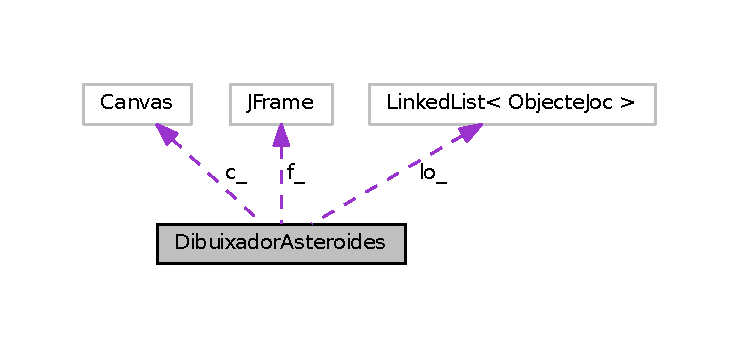
\includegraphics[width=350pt]{class_dibuixador_asteroides__coll__graph}
\end{center}
\end{figure}
\subsection*{Public Member Functions}
\begin{DoxyCompactItemize}
\item 
void \hyperlink{class_dibuixador_asteroides_a54a43290703d14aee21e5c87a5e6fc5b}{crear\+Finestra} (int amplada, int altura, Color fons, String t)
\item 
void \hyperlink{class_dibuixador_asteroides_ac70561df846258437f4145a41117e9ef}{afegir} (\hyperlink{interface_objecte_joc}{Objecte\+Joc} oj)
\item 
void \hyperlink{class_dibuixador_asteroides_a22269129b517ba0da55bc16e19e24b57}{elimina} (\hyperlink{interface_objecte_joc}{Objecte\+Joc} oj)
\item 
void \hyperlink{class_dibuixador_asteroides_a9add2702a95cbe7e68100c97a63b297f}{afegir\+Key\+Listener} (Key\+Listener l)
\item 
void \hyperlink{class_dibuixador_asteroides_af2138b89d2a5fe31697b2f206cbc2df4}{dibuixar} (int puntuacio)
\item 
void \hyperlink{class_dibuixador_asteroides_a14186d7acd8ca135252848f916416575}{tancar\+Finestra} ()
\end{DoxyCompactItemize}
\subsection*{Private Attributes}
\begin{DoxyCompactItemize}
\item 
J\+Frame \hyperlink{class_dibuixador_asteroides_acd1dc7eee6ddda629759fc422566b11b}{f\+\_\+}
\begin{DoxyCompactList}\small\item\em finestra principal \end{DoxyCompactList}\item 
Canvas \hyperlink{class_dibuixador_asteroides_a634f3d95d02d08c9d21d2eef2c3bb410}{c\+\_\+}
\begin{DoxyCompactList}\small\item\em superficie on es dibuixa \end{DoxyCompactList}\item 
Linked\+List$<$ \hyperlink{interface_objecte_joc}{Objecte\+Joc} $>$ \hyperlink{class_dibuixador_asteroides_aafc049ca18d07bf9cf5f61b7e8e1e06f}{lo\+\_\+}
\begin{DoxyCompactList}\small\item\em llista d\textquotesingle{}\hyperlink{interface_objecte_joc}{Objecte\+Joc} \end{DoxyCompactList}\item 
int \hyperlink{class_dibuixador_asteroides_ac5680a5fd826ac9a412b9739f5f64a12}{amplada\+\_\+}
\begin{DoxyCompactList}\small\item\em amplada de c\+\_\+ \end{DoxyCompactList}\end{DoxyCompactItemize}


\subsection{Detailed Description}
Dibuixa multiples \hyperlink{interface_objecte_joc}{Objecte\+Joc} a una finestra. 

La finestra(f) s\textquotesingle{}ha de crear amb \hyperlink{class_dibuixador_asteroides_a54a43290703d14aee21e5c87a5e6fc5b}{crear\+Finestra()}. f té una mida, un color de fons i un titol determinat.

Es pot afegir un Key\+Listener a f

Es poden afegir \hyperlink{interface_objecte_joc}{Objecte\+Joc} a \hyperlink{class_dibuixador_asteroides}{Dibuixador\+Asteroides}. Aquests \hyperlink{interface_objecte_joc}{Objecte\+Joc} es dibuixaran a f

La finestra es pot tornar a crear tantes vegades com es desitji, pero nomes s\textquotesingle{}utilitza la ultima que s\textquotesingle{}ha creat. La finestra es pot tancar en qualsevol moment. 

Definition at line 25 of file Dibuixador\+Asteroides.\+java.



\subsection{Member Function Documentation}
\hypertarget{class_dibuixador_asteroides_ac70561df846258437f4145a41117e9ef}{}\index{Dibuixador\+Asteroides@{Dibuixador\+Asteroides}!afegir@{afegir}}
\index{afegir@{afegir}!Dibuixador\+Asteroides@{Dibuixador\+Asteroides}}
\subsubsection[{afegir}]{\setlength{\rightskip}{0pt plus 5cm}void Dibuixador\+Asteroides.\+afegir (
\begin{DoxyParamCaption}
\item[{{\bf Objecte\+Joc}}]{oj}
\end{DoxyParamCaption}
)}\label{class_dibuixador_asteroides_ac70561df846258437f4145a41117e9ef}
\begin{DoxyPrecond}{Precondition}
--- 
\end{DoxyPrecond}
\begin{DoxyPostcond}{Postcondition}
Si oj no era al \hyperlink{class_dibuixador_asteroides}{Dibuixador\+Asteroides} llavors l\textquotesingle{}afageix altrament no fa res 
\end{DoxyPostcond}


Definition at line 84 of file Dibuixador\+Asteroides.\+java.



Here is the caller graph for this function\+:\nopagebreak
\begin{figure}[H]
\begin{center}
\leavevmode
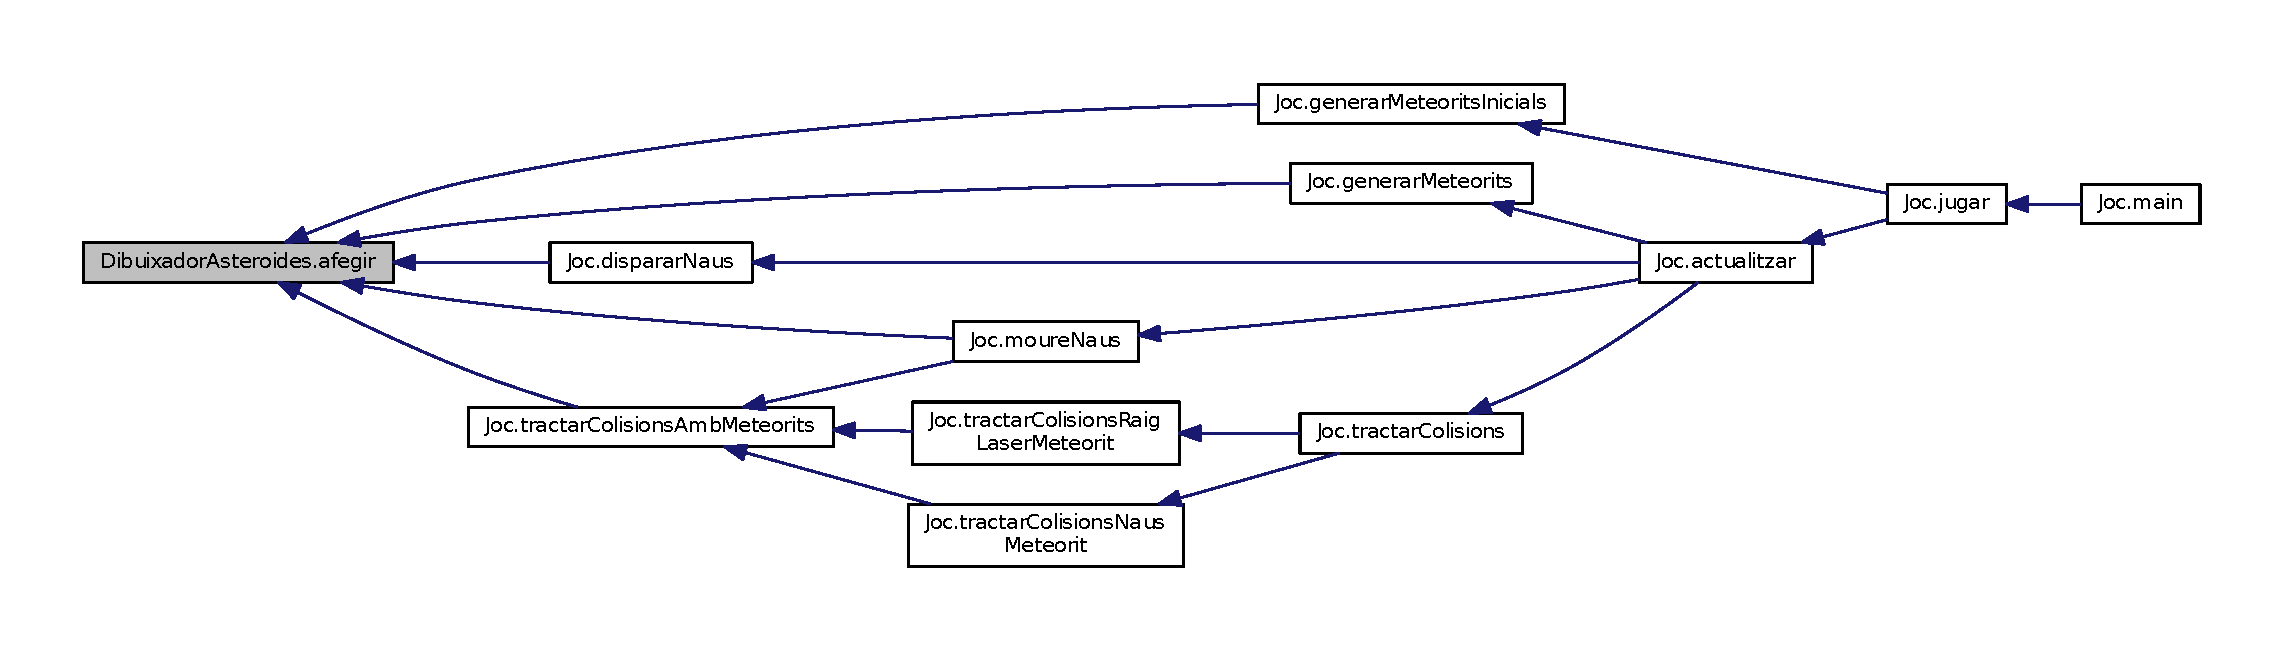
\includegraphics[width=350pt]{class_dibuixador_asteroides_ac70561df846258437f4145a41117e9ef_icgraph}
\end{center}
\end{figure}


\hypertarget{class_dibuixador_asteroides_a9add2702a95cbe7e68100c97a63b297f}{}\index{Dibuixador\+Asteroides@{Dibuixador\+Asteroides}!afegir\+Key\+Listener@{afegir\+Key\+Listener}}
\index{afegir\+Key\+Listener@{afegir\+Key\+Listener}!Dibuixador\+Asteroides@{Dibuixador\+Asteroides}}
\subsubsection[{afegir\+Key\+Listener}]{\setlength{\rightskip}{0pt plus 5cm}void Dibuixador\+Asteroides.\+afegir\+Key\+Listener (
\begin{DoxyParamCaption}
\item[{Key\+Listener}]{l}
\end{DoxyParamCaption}
)}\label{class_dibuixador_asteroides_a9add2702a95cbe7e68100c97a63b297f}
\begin{DoxyPrecond}{Precondition}
--- 
\end{DoxyPrecond}
\begin{DoxyPostcond}{Postcondition}
afageix l a la finestra del Dibuixa\+Asteroides 
\end{DoxyPostcond}


Definition at line 100 of file Dibuixador\+Asteroides.\+java.

\hypertarget{class_dibuixador_asteroides_a54a43290703d14aee21e5c87a5e6fc5b}{}\index{Dibuixador\+Asteroides@{Dibuixador\+Asteroides}!crear\+Finestra@{crear\+Finestra}}
\index{crear\+Finestra@{crear\+Finestra}!Dibuixador\+Asteroides@{Dibuixador\+Asteroides}}
\subsubsection[{crear\+Finestra}]{\setlength{\rightskip}{0pt plus 5cm}void Dibuixador\+Asteroides.\+crear\+Finestra (
\begin{DoxyParamCaption}
\item[{int}]{amplada, }
\item[{int}]{altura, }
\item[{Color}]{fons, }
\item[{String}]{t}
\end{DoxyParamCaption}
)}\label{class_dibuixador_asteroides_a54a43290703d14aee21e5c87a5e6fc5b}
\begin{DoxyPrecond}{Precondition}
-- 
\end{DoxyPrecond}
\begin{DoxyPostcond}{Postcondition}
crea una finestra per al Dibuixa\+Asteroides amb una superficie amplada x altura, el color de fons es {\itshape fons} i el titol és t 
\end{DoxyPostcond}


Definition at line 58 of file Dibuixador\+Asteroides.\+java.

\hypertarget{class_dibuixador_asteroides_af2138b89d2a5fe31697b2f206cbc2df4}{}\index{Dibuixador\+Asteroides@{Dibuixador\+Asteroides}!dibuixar@{dibuixar}}
\index{dibuixar@{dibuixar}!Dibuixador\+Asteroides@{Dibuixador\+Asteroides}}
\subsubsection[{dibuixar}]{\setlength{\rightskip}{0pt plus 5cm}void Dibuixador\+Asteroides.\+dibuixar (
\begin{DoxyParamCaption}
\item[{int}]{puntuacio}
\end{DoxyParamCaption}
)}\label{class_dibuixador_asteroides_af2138b89d2a5fe31697b2f206cbc2df4}
\begin{DoxyPrecond}{Precondition}
finestra creada 
\end{DoxyPrecond}
\begin{DoxyPostcond}{Postcondition}
pinta a la superficie de la finestra del Dibuixa\+Asteroides amb el color de fons i pinta tots els \hyperlink{interface_objecte_joc}{Objecte\+Joc} que s\textquotesingle{}han afegit al Dibuixa\+Asteroides. També mostra puntuacio al costat esquerre superior. 
\end{DoxyPostcond}


Definition at line 108 of file Dibuixador\+Asteroides.\+java.



Here is the caller graph for this function\+:\nopagebreak
\begin{figure}[H]
\begin{center}
\leavevmode
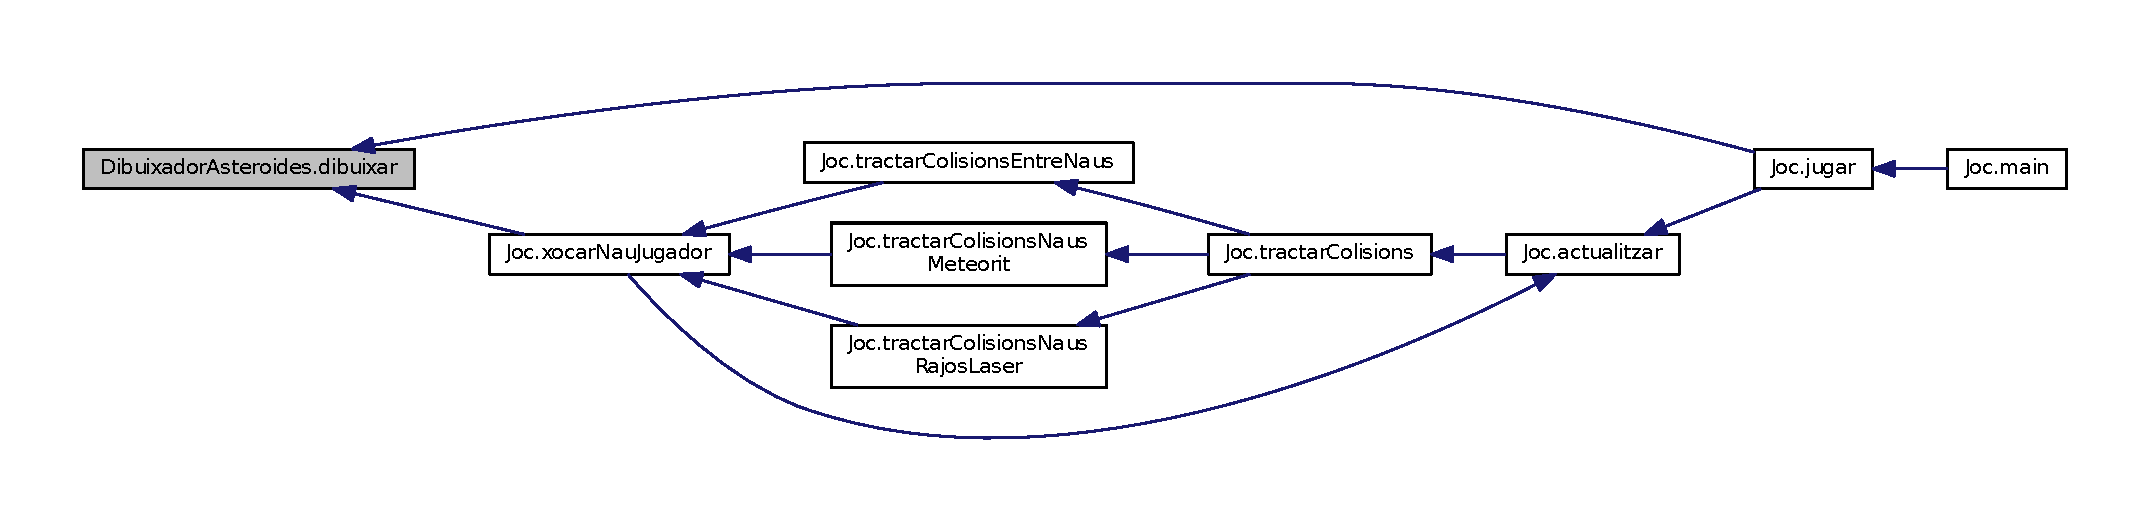
\includegraphics[width=350pt]{class_dibuixador_asteroides_af2138b89d2a5fe31697b2f206cbc2df4_icgraph}
\end{center}
\end{figure}


\hypertarget{class_dibuixador_asteroides_a22269129b517ba0da55bc16e19e24b57}{}\index{Dibuixador\+Asteroides@{Dibuixador\+Asteroides}!elimina@{elimina}}
\index{elimina@{elimina}!Dibuixador\+Asteroides@{Dibuixador\+Asteroides}}
\subsubsection[{elimina}]{\setlength{\rightskip}{0pt plus 5cm}void Dibuixador\+Asteroides.\+elimina (
\begin{DoxyParamCaption}
\item[{{\bf Objecte\+Joc}}]{oj}
\end{DoxyParamCaption}
)}\label{class_dibuixador_asteroides_a22269129b517ba0da55bc16e19e24b57}
\begin{DoxyPrecond}{Precondition}
--- 
\end{DoxyPrecond}
\begin{DoxyPostcond}{Postcondition}
Si oj era al \hyperlink{class_dibuixador_asteroides}{Dibuixador\+Asteroides} llavors l\textquotesingle{}elimina altrament no fa res 
\end{DoxyPostcond}


Definition at line 92 of file Dibuixador\+Asteroides.\+java.



Here is the caller graph for this function\+:\nopagebreak
\begin{figure}[H]
\begin{center}
\leavevmode
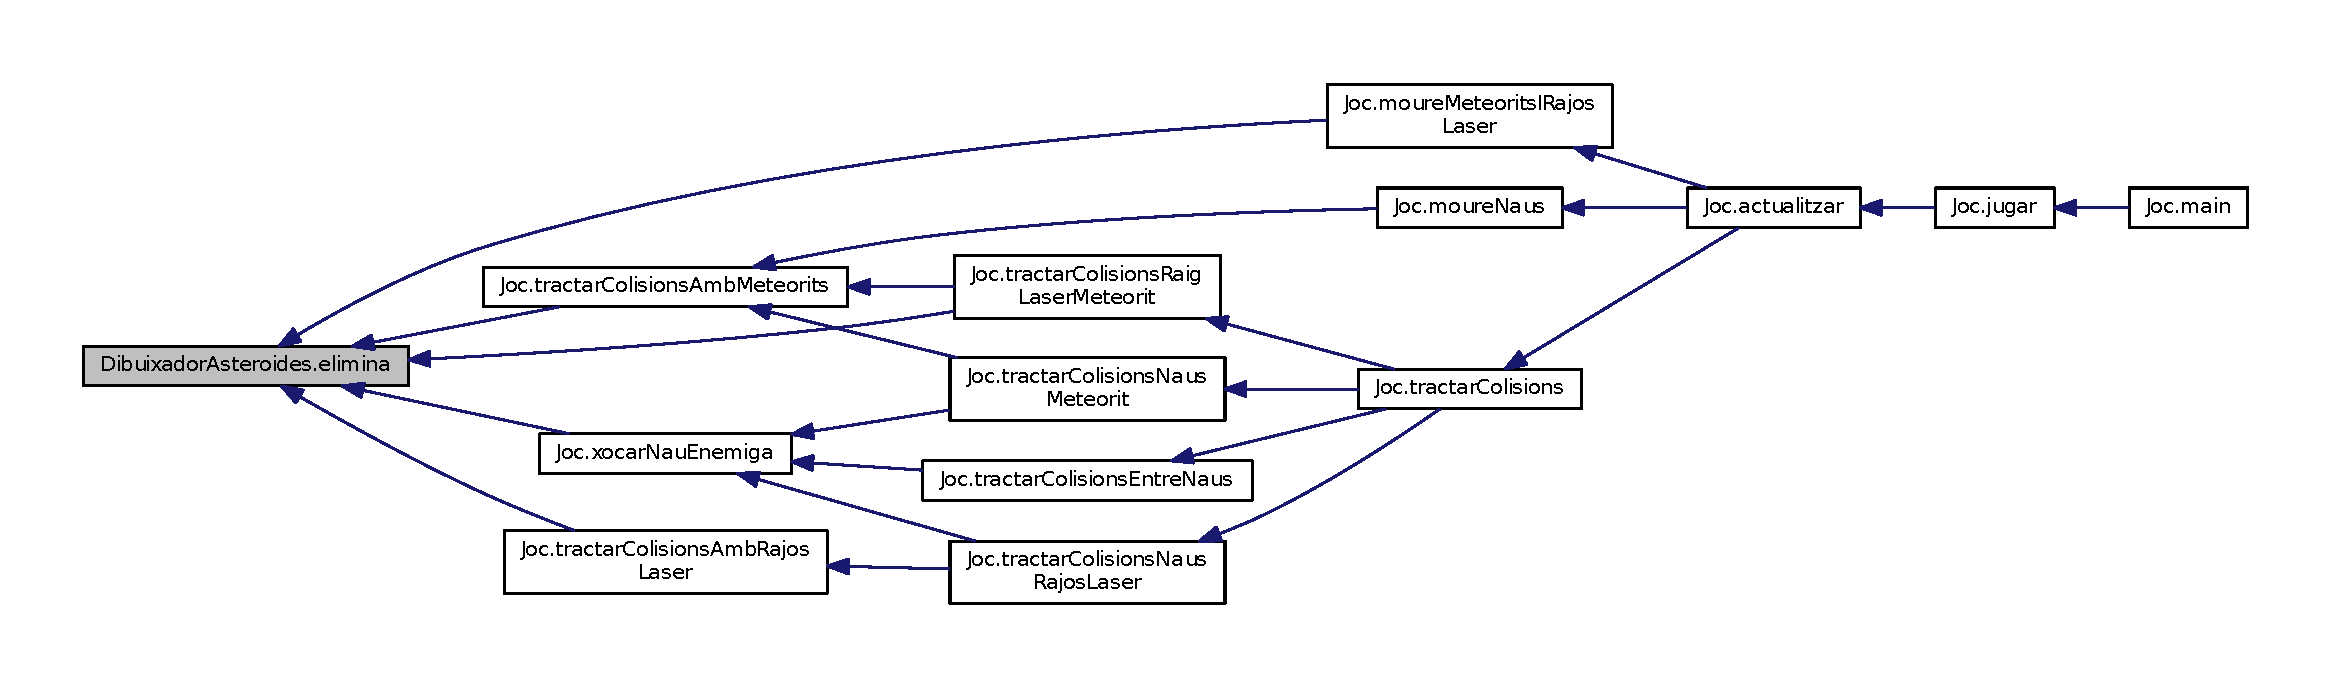
\includegraphics[width=350pt]{class_dibuixador_asteroides_a22269129b517ba0da55bc16e19e24b57_icgraph}
\end{center}
\end{figure}


\hypertarget{class_dibuixador_asteroides_a14186d7acd8ca135252848f916416575}{}\index{Dibuixador\+Asteroides@{Dibuixador\+Asteroides}!tancar\+Finestra@{tancar\+Finestra}}
\index{tancar\+Finestra@{tancar\+Finestra}!Dibuixador\+Asteroides@{Dibuixador\+Asteroides}}
\subsubsection[{tancar\+Finestra}]{\setlength{\rightskip}{0pt plus 5cm}void Dibuixador\+Asteroides.\+tancar\+Finestra (
\begin{DoxyParamCaption}
{}
\end{DoxyParamCaption}
)}\label{class_dibuixador_asteroides_a14186d7acd8ca135252848f916416575}
\begin{DoxyPrecond}{Precondition}
el Dibuixa\+Asteroides té finestra 
\end{DoxyPrecond}
\begin{DoxyPostcond}{Postcondition}
s\textquotesingle{}ha tancat la finestra del Dibuixa\+Asteroides 
\end{DoxyPostcond}


Definition at line 131 of file Dibuixador\+Asteroides.\+java.



Here is the caller graph for this function\+:\nopagebreak
\begin{figure}[H]
\begin{center}
\leavevmode
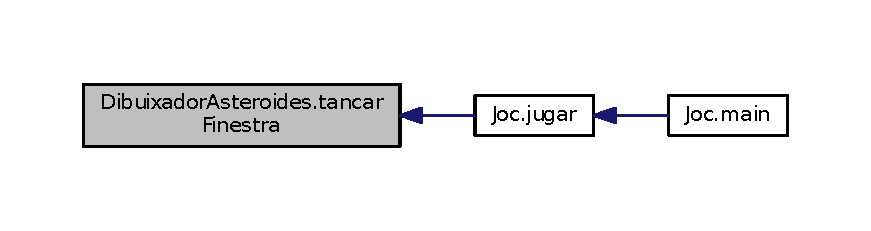
\includegraphics[width=350pt]{class_dibuixador_asteroides_a14186d7acd8ca135252848f916416575_icgraph}
\end{center}
\end{figure}




\subsection{Member Data Documentation}
\hypertarget{class_dibuixador_asteroides_ac5680a5fd826ac9a412b9739f5f64a12}{}\index{Dibuixador\+Asteroides@{Dibuixador\+Asteroides}!amplada\+\_\+@{amplada\+\_\+}}
\index{amplada\+\_\+@{amplada\+\_\+}!Dibuixador\+Asteroides@{Dibuixador\+Asteroides}}
\subsubsection[{amplada\+\_\+}]{\setlength{\rightskip}{0pt plus 5cm}int Dibuixador\+Asteroides.\+amplada\+\_\+\hspace{0.3cm}{\ttfamily [private]}}\label{class_dibuixador_asteroides_ac5680a5fd826ac9a412b9739f5f64a12}


amplada de c\+\_\+ 



Definition at line 44 of file Dibuixador\+Asteroides.\+java.

\hypertarget{class_dibuixador_asteroides_a634f3d95d02d08c9d21d2eef2c3bb410}{}\index{Dibuixador\+Asteroides@{Dibuixador\+Asteroides}!c\+\_\+@{c\+\_\+}}
\index{c\+\_\+@{c\+\_\+}!Dibuixador\+Asteroides@{Dibuixador\+Asteroides}}
\subsubsection[{c\+\_\+}]{\setlength{\rightskip}{0pt plus 5cm}Canvas Dibuixador\+Asteroides.\+c\+\_\+\hspace{0.3cm}{\ttfamily [private]}}\label{class_dibuixador_asteroides_a634f3d95d02d08c9d21d2eef2c3bb410}


superficie on es dibuixa 



Definition at line 42 of file Dibuixador\+Asteroides.\+java.

\hypertarget{class_dibuixador_asteroides_acd1dc7eee6ddda629759fc422566b11b}{}\index{Dibuixador\+Asteroides@{Dibuixador\+Asteroides}!f\+\_\+@{f\+\_\+}}
\index{f\+\_\+@{f\+\_\+}!Dibuixador\+Asteroides@{Dibuixador\+Asteroides}}
\subsubsection[{f\+\_\+}]{\setlength{\rightskip}{0pt plus 5cm}J\+Frame Dibuixador\+Asteroides.\+f\+\_\+\hspace{0.3cm}{\ttfamily [private]}}\label{class_dibuixador_asteroides_acd1dc7eee6ddda629759fc422566b11b}


finestra principal 



Definition at line 41 of file Dibuixador\+Asteroides.\+java.

\hypertarget{class_dibuixador_asteroides_aafc049ca18d07bf9cf5f61b7e8e1e06f}{}\index{Dibuixador\+Asteroides@{Dibuixador\+Asteroides}!lo\+\_\+@{lo\+\_\+}}
\index{lo\+\_\+@{lo\+\_\+}!Dibuixador\+Asteroides@{Dibuixador\+Asteroides}}
\subsubsection[{lo\+\_\+}]{\setlength{\rightskip}{0pt plus 5cm}Linked\+List$<$ {\bf Objecte\+Joc} $>$ Dibuixador\+Asteroides.\+lo\+\_\+\hspace{0.3cm}{\ttfamily [private]}}\label{class_dibuixador_asteroides_aafc049ca18d07bf9cf5f61b7e8e1e06f}


llista d\textquotesingle{}\hyperlink{interface_objecte_joc}{Objecte\+Joc} 



Definition at line 43 of file Dibuixador\+Asteroides.\+java.



The documentation for this class was generated from the following file\+:\begin{DoxyCompactItemize}
\item 
/mnt/\+Dades/\+Documents/uni/\+Pro\+P/asteroides/src/\hyperlink{_dibuixador_asteroides_8java}{Dibuixador\+Asteroides.\+java}\end{DoxyCompactItemize}

\hypertarget{class_joc}{}\section{Joc Class Reference}
\label{class_joc}\index{Joc@{Joc}}


Collaboration diagram for Joc\+:\nopagebreak
\begin{figure}[H]
\begin{center}
\leavevmode
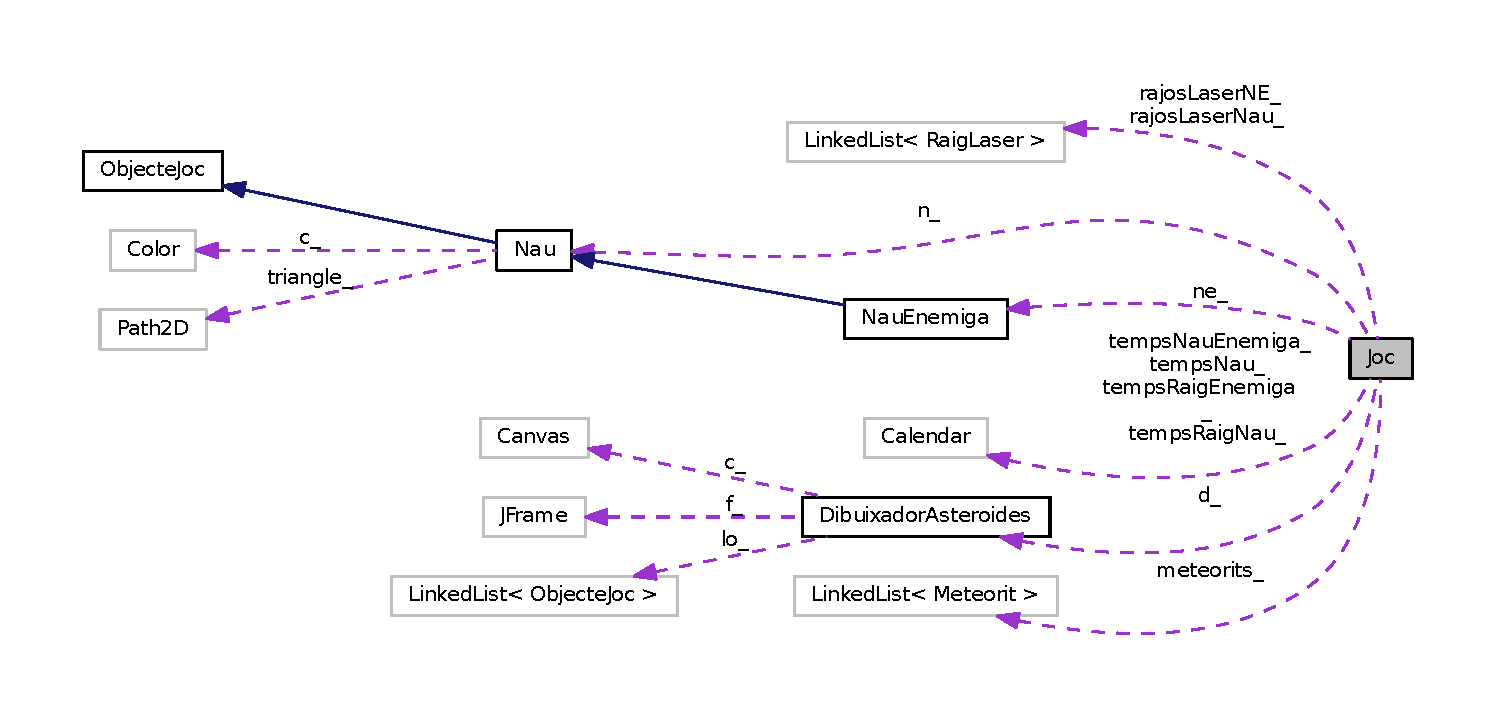
\includegraphics[width=350pt]{class_joc__coll__graph}
\end{center}
\end{figure}
\subsection*{Classes}
\begin{DoxyCompactItemize}
\item 
class \hyperlink{class_joc_1_1_my_key_listener}{My\+Key\+Listener}
\begin{DoxyCompactList}\small\item\em Key\+Listener per a actualitzar els booleans segons les pulsacions del teclat. \end{DoxyCompactList}\end{DoxyCompactItemize}
\subsection*{Public Member Functions}
\begin{DoxyCompactItemize}
\item 
void \hyperlink{class_joc_aa5da4464cac2dc81f26430ac16fa7029}{jugar} ()  throws Exception 
\end{DoxyCompactItemize}
\subsection*{Static Public Member Functions}
\begin{DoxyCompactItemize}
\item 
static void \hyperlink{class_joc_a54cbe41c97ce7489f7b0cc62217a7d29}{main} (String\mbox{[}$\,$\mbox{]} args)  throws Exception 
\end{DoxyCompactItemize}
\subsection*{Private Member Functions}
\begin{DoxyCompactItemize}
\item 
void \hyperlink{class_joc_ab4169a454c9b3b6b6030fd785483a15d}{generar\+Meteorits\+Inicials} ()  throws Exception 
\item 
void \hyperlink{class_joc_afb711913c78395c05839c3f775792beb}{generar\+Meteorits} ()  throws Exception 
\item 
void \hyperlink{class_joc_aafe85787281ae19be9ee44aabc5c116c}{actualitzar} ()  throws Exception 
\item 
void \hyperlink{class_joc_a82b3c98f504183b2ade08ae6f7fbbdce}{disparar\+Naus} ()  throws Exception 
\item 
void \hyperlink{class_joc_a9b0d8fa2d2613d958dc8bf650ae78a34}{moure\+Naus} ()  throws Exception 
\item 
void \hyperlink{class_joc_af9e0ddcc5b82db8ff4d07bbd443c7f8d}{moure\+Meteorits\+I\+Rajos\+Laser} ()  throws Exception 
\item 
void \hyperlink{class_joc_a1be330c10f1e2ee06f696e0a0bdec7c7}{tractar\+Colisions} ()  throws Exception 
\item 
void \hyperlink{class_joc_a471c58ad94b7a8732a6b3e4695f2a691}{xocar\+Nau\+Jugador} ()  throws Exception 
\item 
void \hyperlink{class_joc_a84da80994a7dd370b3772cf962500617}{xocar\+Nau\+Enemiga} ()  throws Exception 
\item 
void \hyperlink{class_joc_abc5db47ede50ddeccb50b2872d05cb6c}{tractar\+Colisions\+Entre\+Naus} ()  throws Exception 
\item 
void \hyperlink{class_joc_a9a3116242cc69985726f4825be70a9b5}{tractar\+Colisions\+Raig\+Laser\+Nau\+Meteorit} ()  throws Exception 
\item 
void \hyperlink{class_joc_af717aa44d1134343a67fc08374c3af45}{tractar\+Colisions\+Raig\+Laser\+N\+E\+Meteorit} ()  throws Exception 
\item 
boolean \hyperlink{class_joc_a16b0be1ee6298106946df8150044f667}{tractar\+Colisions\+Amb\+Meteorits} (Area a, boolean puntuar)  throws Exception 
\item 
void \hyperlink{class_joc_acf31c665e8f734f15f40f8e6792e8bba}{tractar\+Colisions\+Naus\+Meteorit} ()  throws Exception 
\item 
void \hyperlink{class_joc_a9ccc5adec1e7efdd6c01ba393d3686c6}{tractar\+Colisions\+Naus\+Rajos\+Laser} ()  throws Exception 
\item 
boolean \hyperlink{class_joc_ac94f4a327797f506171f0db74b3feaee}{tractar\+Colisions\+Amb\+Rajos\+Laser} (Area a)  throws Exception 
\end{DoxyCompactItemize}


\subsection{Detailed Description}


Definition at line 75 of file Joc.\+java.



\subsection{Member Function Documentation}
\hypertarget{class_joc_aafe85787281ae19be9ee44aabc5c116c}{}\index{Joc@{Joc}!actualitzar@{actualitzar}}
\index{actualitzar@{actualitzar}!Joc@{Joc}}
\subsubsection[{actualitzar}]{\setlength{\rightskip}{0pt plus 5cm}void Joc.\+actualitzar (
\begin{DoxyParamCaption}
{}
\end{DoxyParamCaption}
) throws Exception\hspace{0.3cm}{\ttfamily [private]}}\label{class_joc_aafe85787281ae19be9ee44aabc5c116c}
\begin{DoxyPrecond}{Precondition}
-- 
\end{DoxyPrecond}
\begin{DoxyPostcond}{Postcondition}
actualitza l\textquotesingle{}estat del joc, generant meteorits, movent els elements i tractant les col·lisions 
\end{DoxyPostcond}


Definition at line 254 of file Joc.\+java.



Here is the call graph for this function\+:\nopagebreak
\begin{figure}[H]
\begin{center}
\leavevmode
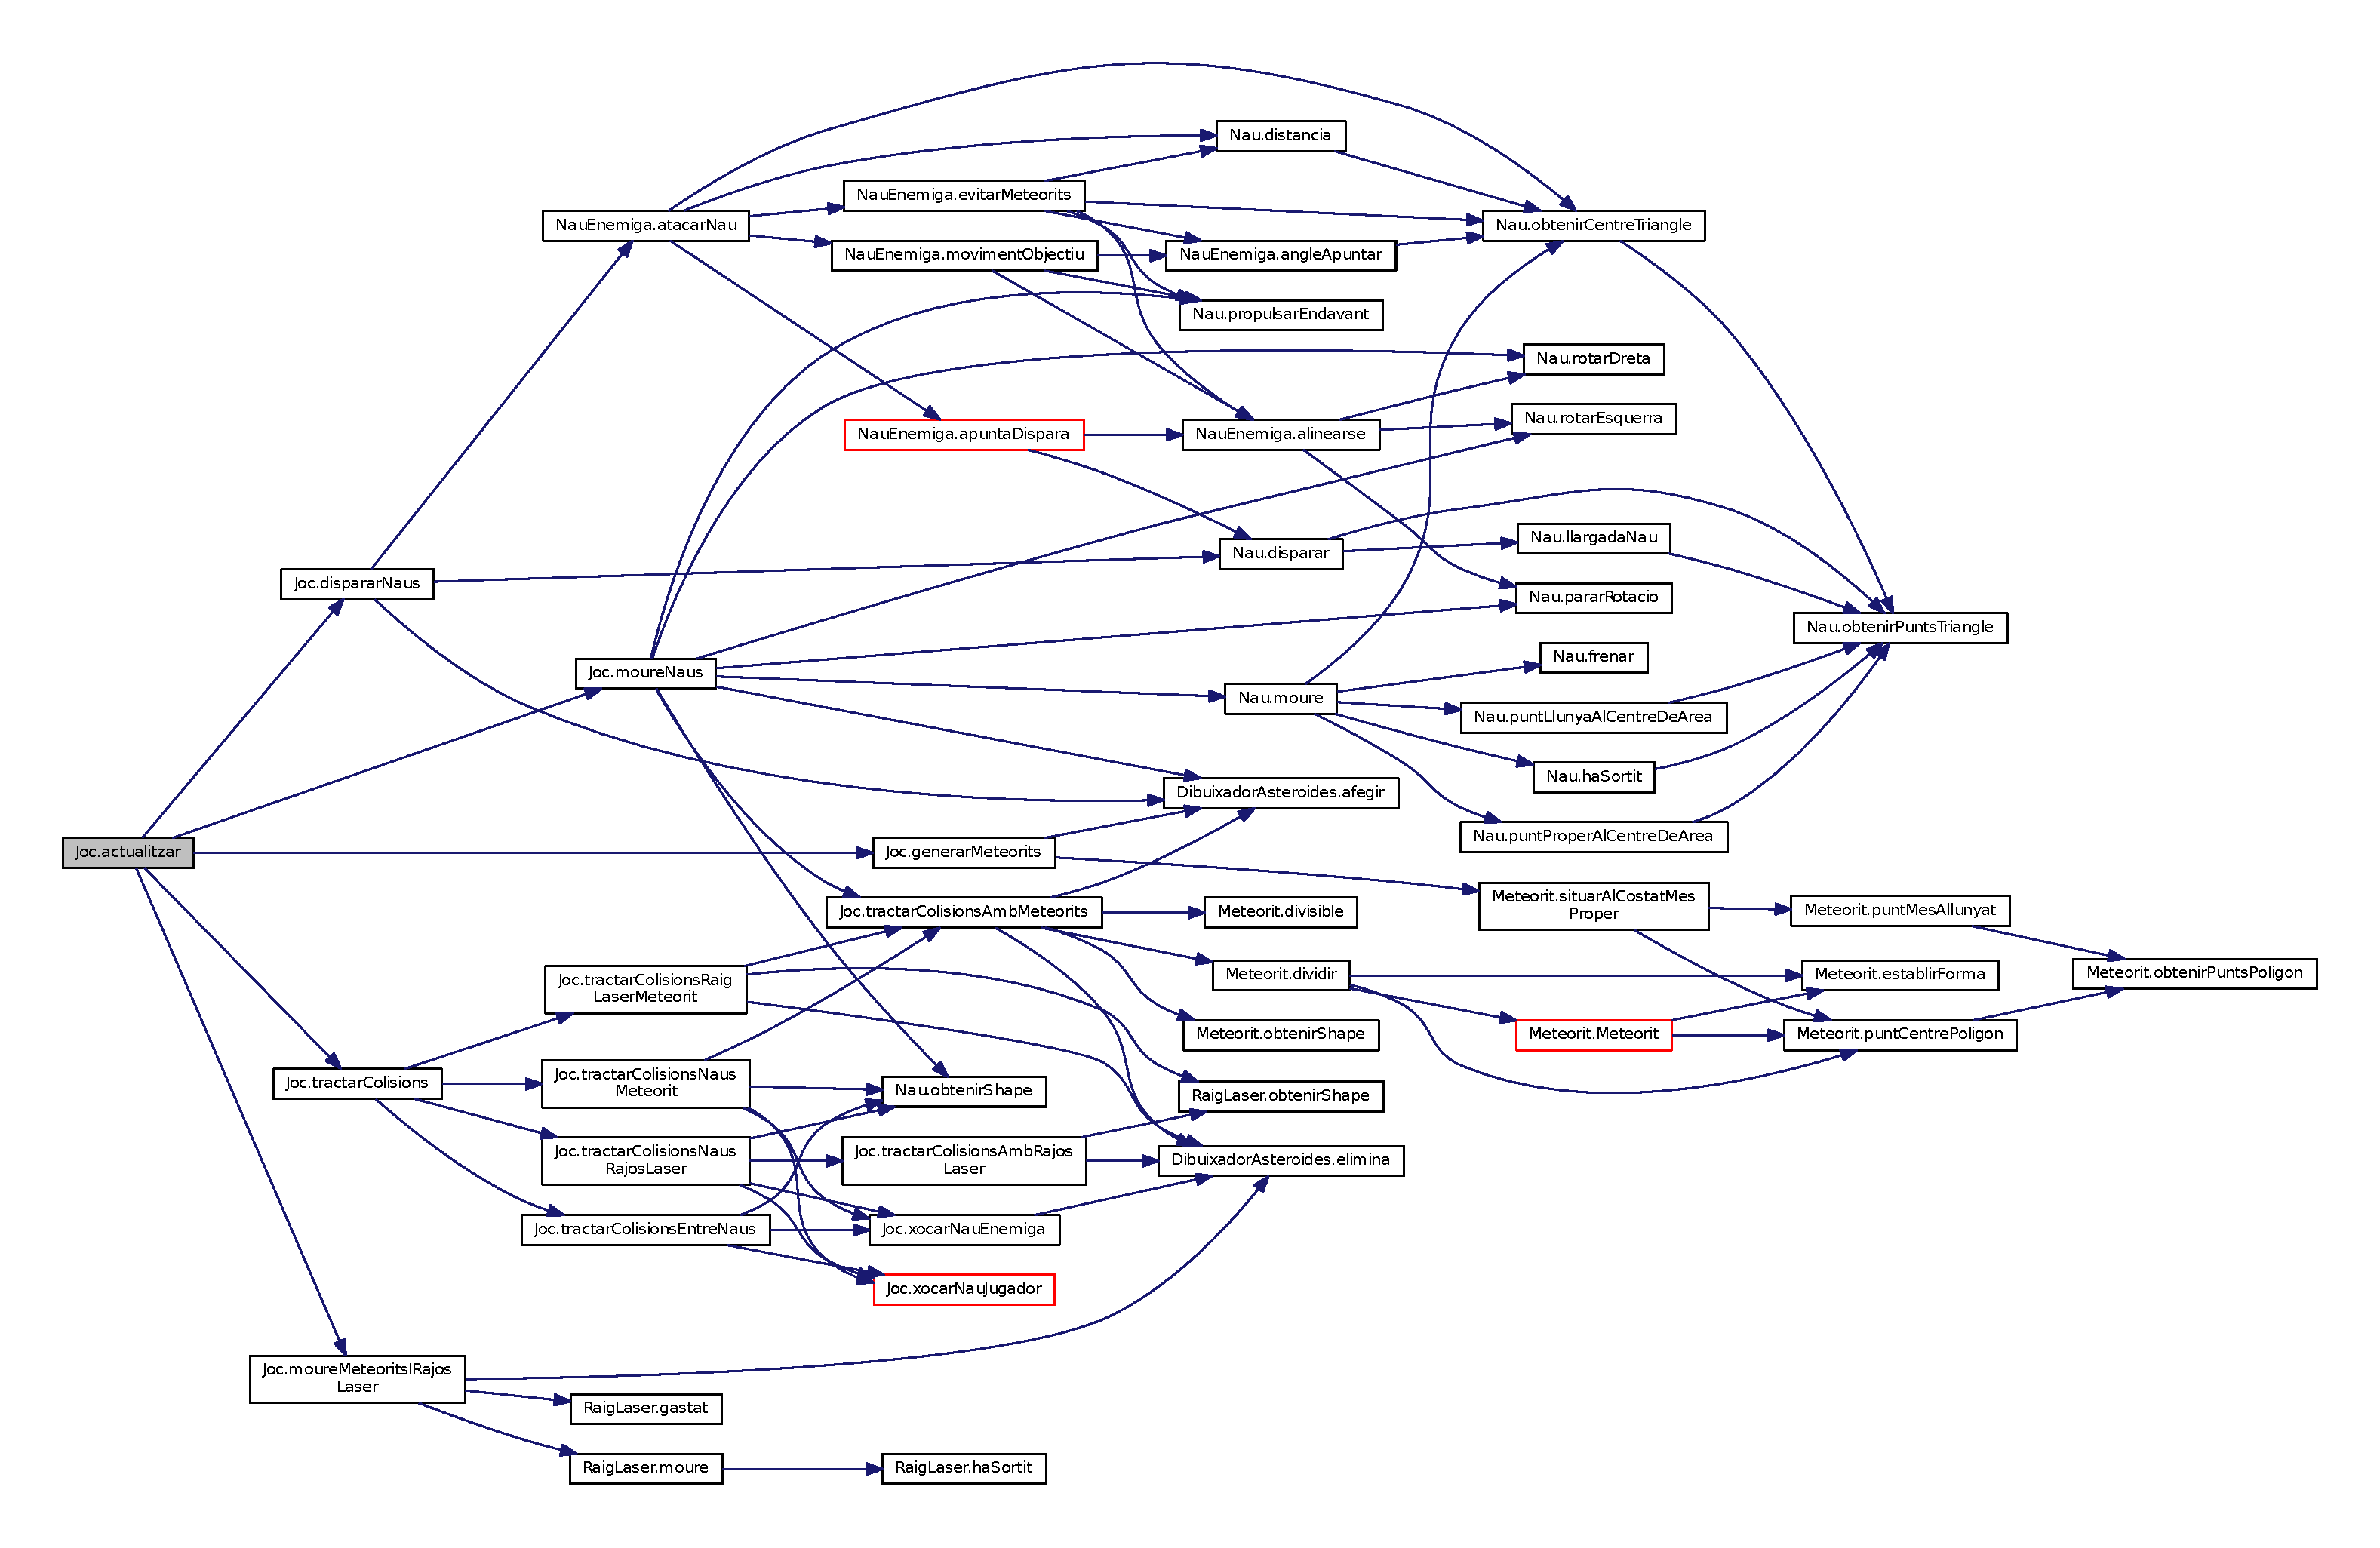
\includegraphics[width=350pt]{class_joc_aafe85787281ae19be9ee44aabc5c116c_cgraph}
\end{center}
\end{figure}




Here is the caller graph for this function\+:\nopagebreak
\begin{figure}[H]
\begin{center}
\leavevmode
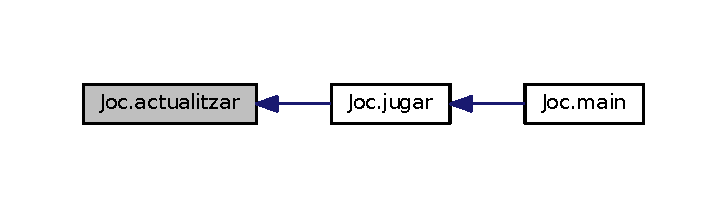
\includegraphics[width=350pt]{class_joc_aafe85787281ae19be9ee44aabc5c116c_icgraph}
\end{center}
\end{figure}


\hypertarget{class_joc_a82b3c98f504183b2ade08ae6f7fbbdce}{}\index{Joc@{Joc}!disparar\+Naus@{disparar\+Naus}}
\index{disparar\+Naus@{disparar\+Naus}!Joc@{Joc}}
\subsubsection[{disparar\+Naus}]{\setlength{\rightskip}{0pt plus 5cm}void Joc.\+disparar\+Naus (
\begin{DoxyParamCaption}
{}
\end{DoxyParamCaption}
) throws Exception\hspace{0.3cm}{\ttfamily [private]}}\label{class_joc_a82b3c98f504183b2ade08ae6f7fbbdce}
\begin{DoxyPrecond}{Precondition}
-- 
\end{DoxyPrecond}
\begin{DoxyPostcond}{Postcondition}
si la \hyperlink{class_nau}{Nau} ha de disparar, dispara i afegeix el \hyperlink{class_raig_laser}{Raig\+Laser} a la llista de \hyperlink{class_raig_laser}{Raig\+Laser} del \hyperlink{class_joc}{Joc}, fent el mateix amb la \hyperlink{class_nau_enemiga}{Nau\+Enemiga} 
\end{DoxyPostcond}


Definition at line 269 of file Joc.\+java.



Here is the call graph for this function\+:\nopagebreak
\begin{figure}[H]
\begin{center}
\leavevmode
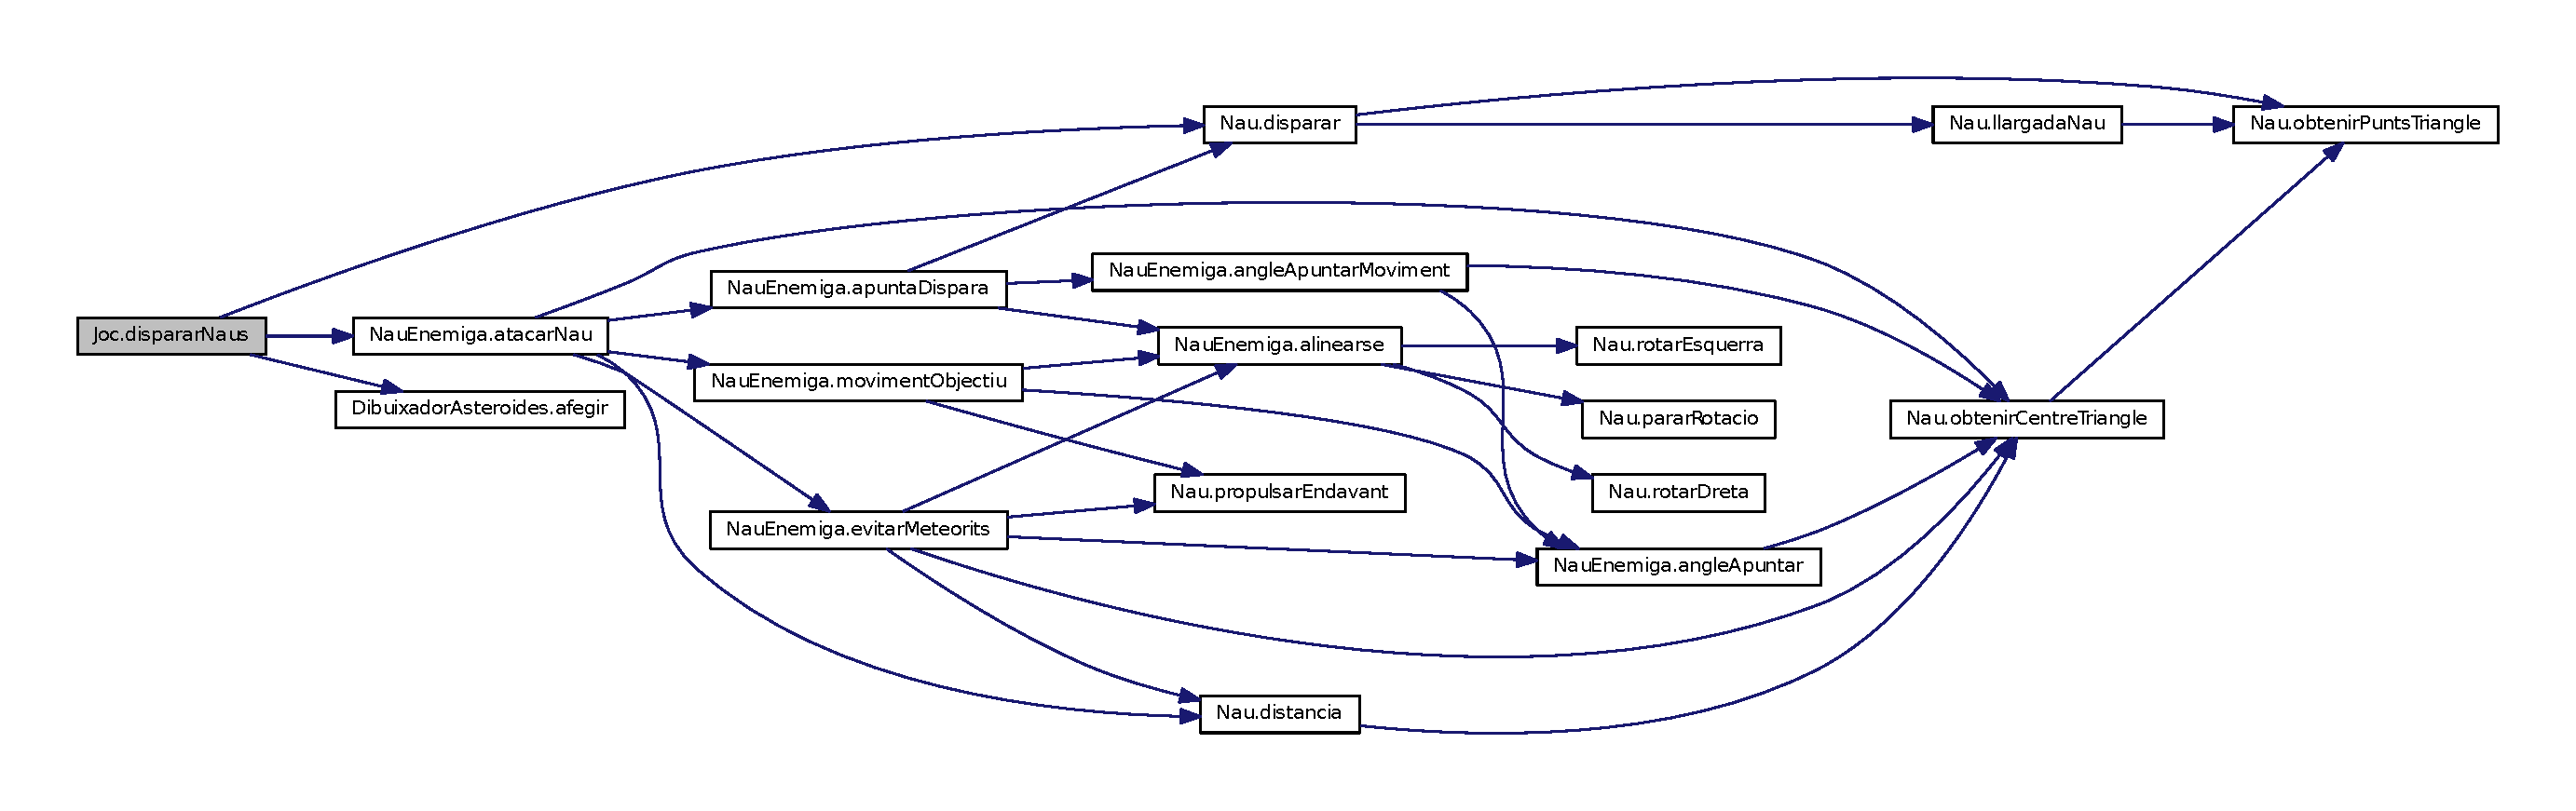
\includegraphics[width=350pt]{class_joc_a82b3c98f504183b2ade08ae6f7fbbdce_cgraph}
\end{center}
\end{figure}




Here is the caller graph for this function\+:\nopagebreak
\begin{figure}[H]
\begin{center}
\leavevmode
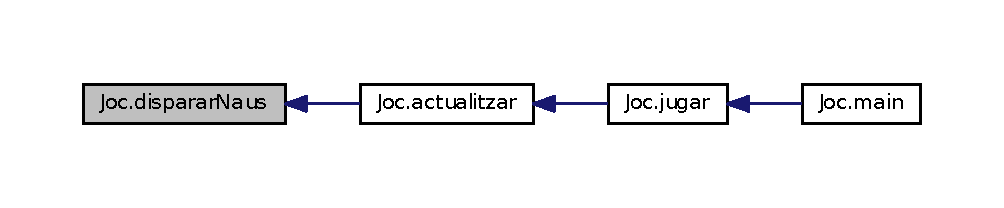
\includegraphics[width=350pt]{class_joc_a82b3c98f504183b2ade08ae6f7fbbdce_icgraph}
\end{center}
\end{figure}


\hypertarget{class_joc_afb711913c78395c05839c3f775792beb}{}\index{Joc@{Joc}!generar\+Meteorits@{generar\+Meteorits}}
\index{generar\+Meteorits@{generar\+Meteorits}!Joc@{Joc}}
\subsubsection[{generar\+Meteorits}]{\setlength{\rightskip}{0pt plus 5cm}void Joc.\+generar\+Meteorits (
\begin{DoxyParamCaption}
{}
\end{DoxyParamCaption}
) throws Exception\hspace{0.3cm}{\ttfamily [private]}}\label{class_joc_afb711913c78395c05839c3f775792beb}
\begin{DoxyPrecond}{Precondition}
-- 
\end{DoxyPrecond}
\begin{DoxyPostcond}{Postcondition}
afegeix Meteorits al \hyperlink{class_dibuixador_asteroides}{Dibuixador\+Asteroides} i al \hyperlink{class_joc}{Joc}, fins a un màxim de 8, i els fa sortir per les bandes de la pantalla 
\end{DoxyPostcond}


Definition at line 242 of file Joc.\+java.



Here is the call graph for this function\+:\nopagebreak
\begin{figure}[H]
\begin{center}
\leavevmode
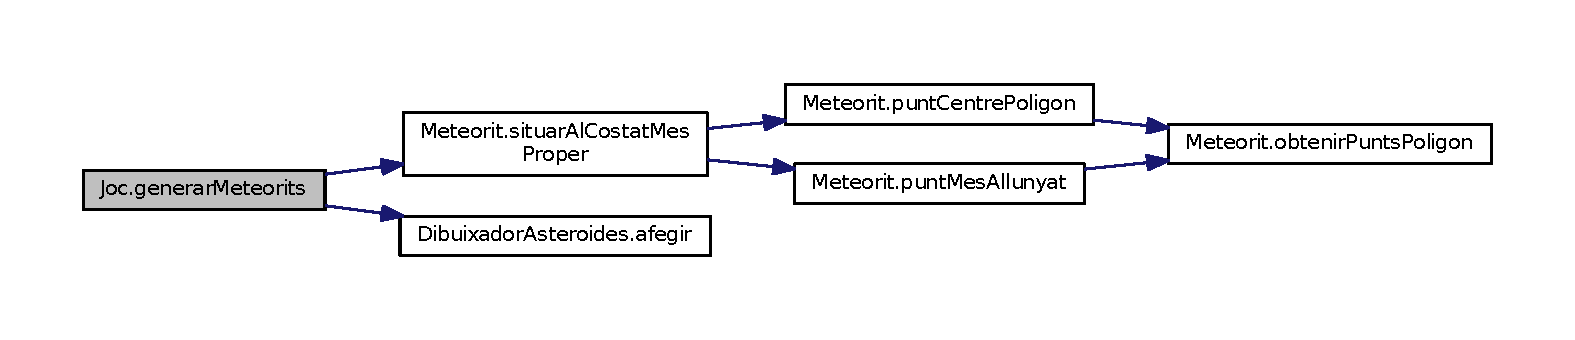
\includegraphics[width=350pt]{class_joc_afb711913c78395c05839c3f775792beb_cgraph}
\end{center}
\end{figure}




Here is the caller graph for this function\+:\nopagebreak
\begin{figure}[H]
\begin{center}
\leavevmode
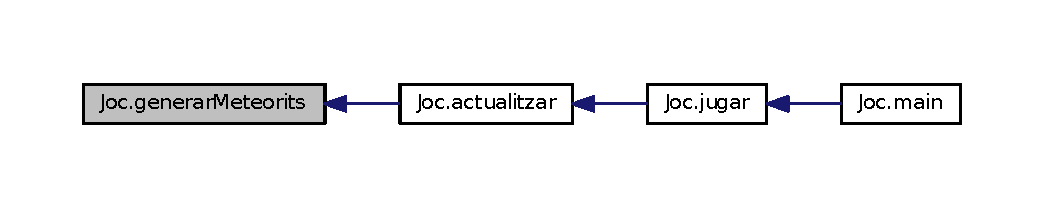
\includegraphics[width=350pt]{class_joc_afb711913c78395c05839c3f775792beb_icgraph}
\end{center}
\end{figure}


\hypertarget{class_joc_ab4169a454c9b3b6b6030fd785483a15d}{}\index{Joc@{Joc}!generar\+Meteorits\+Inicials@{generar\+Meteorits\+Inicials}}
\index{generar\+Meteorits\+Inicials@{generar\+Meteorits\+Inicials}!Joc@{Joc}}
\subsubsection[{generar\+Meteorits\+Inicials}]{\setlength{\rightskip}{0pt plus 5cm}void Joc.\+generar\+Meteorits\+Inicials (
\begin{DoxyParamCaption}
{}
\end{DoxyParamCaption}
) throws Exception\hspace{0.3cm}{\ttfamily [private]}}\label{class_joc_ab4169a454c9b3b6b6030fd785483a15d}
\begin{DoxyPrecond}{Precondition}
-- 
\end{DoxyPrecond}
\begin{DoxyPostcond}{Postcondition}
afegeix Meteorits al \hyperlink{class_dibuixador_asteroides}{Dibuixador\+Asteroides} i al \hyperlink{class_joc}{Joc}, fins a un màxim de 8, evitant que estiguin sobre la \hyperlink{class_nau}{Nau} 
\end{DoxyPostcond}


Definition at line 224 of file Joc.\+java.



Here is the call graph for this function\+:\nopagebreak
\begin{figure}[H]
\begin{center}
\leavevmode
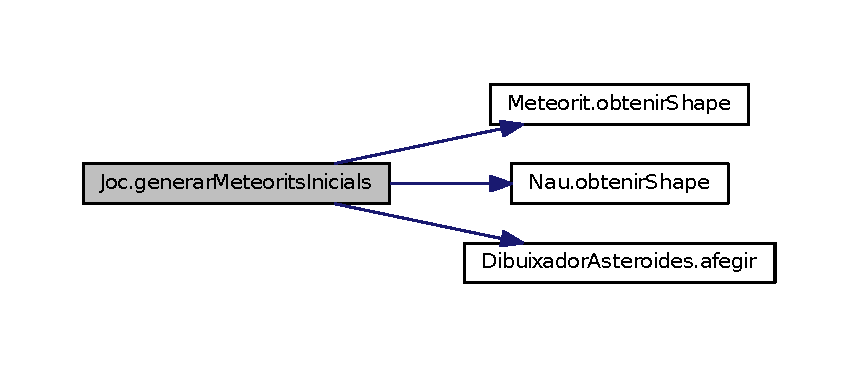
\includegraphics[width=350pt]{class_joc_ab4169a454c9b3b6b6030fd785483a15d_cgraph}
\end{center}
\end{figure}




Here is the caller graph for this function\+:\nopagebreak
\begin{figure}[H]
\begin{center}
\leavevmode
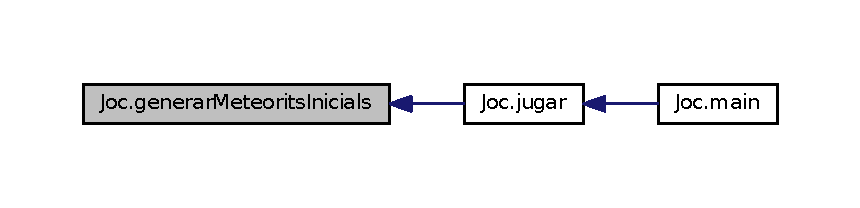
\includegraphics[width=350pt]{class_joc_ab4169a454c9b3b6b6030fd785483a15d_icgraph}
\end{center}
\end{figure}


\hypertarget{class_joc_aa5da4464cac2dc81f26430ac16fa7029}{}\index{Joc@{Joc}!jugar@{jugar}}
\index{jugar@{jugar}!Joc@{Joc}}
\subsubsection[{jugar}]{\setlength{\rightskip}{0pt plus 5cm}void Joc.\+jugar (
\begin{DoxyParamCaption}
{}
\end{DoxyParamCaption}
) throws Exception}\label{class_joc_aa5da4464cac2dc81f26430ac16fa7029}
\begin{DoxyPrecond}{Precondition}
-- 
\end{DoxyPrecond}
\begin{DoxyPostcond}{Postcondition}
es comença a jugar la partida 
\end{DoxyPostcond}


Definition at line 201 of file Joc.\+java.



Here is the call graph for this function\+:\nopagebreak
\begin{figure}[H]
\begin{center}
\leavevmode
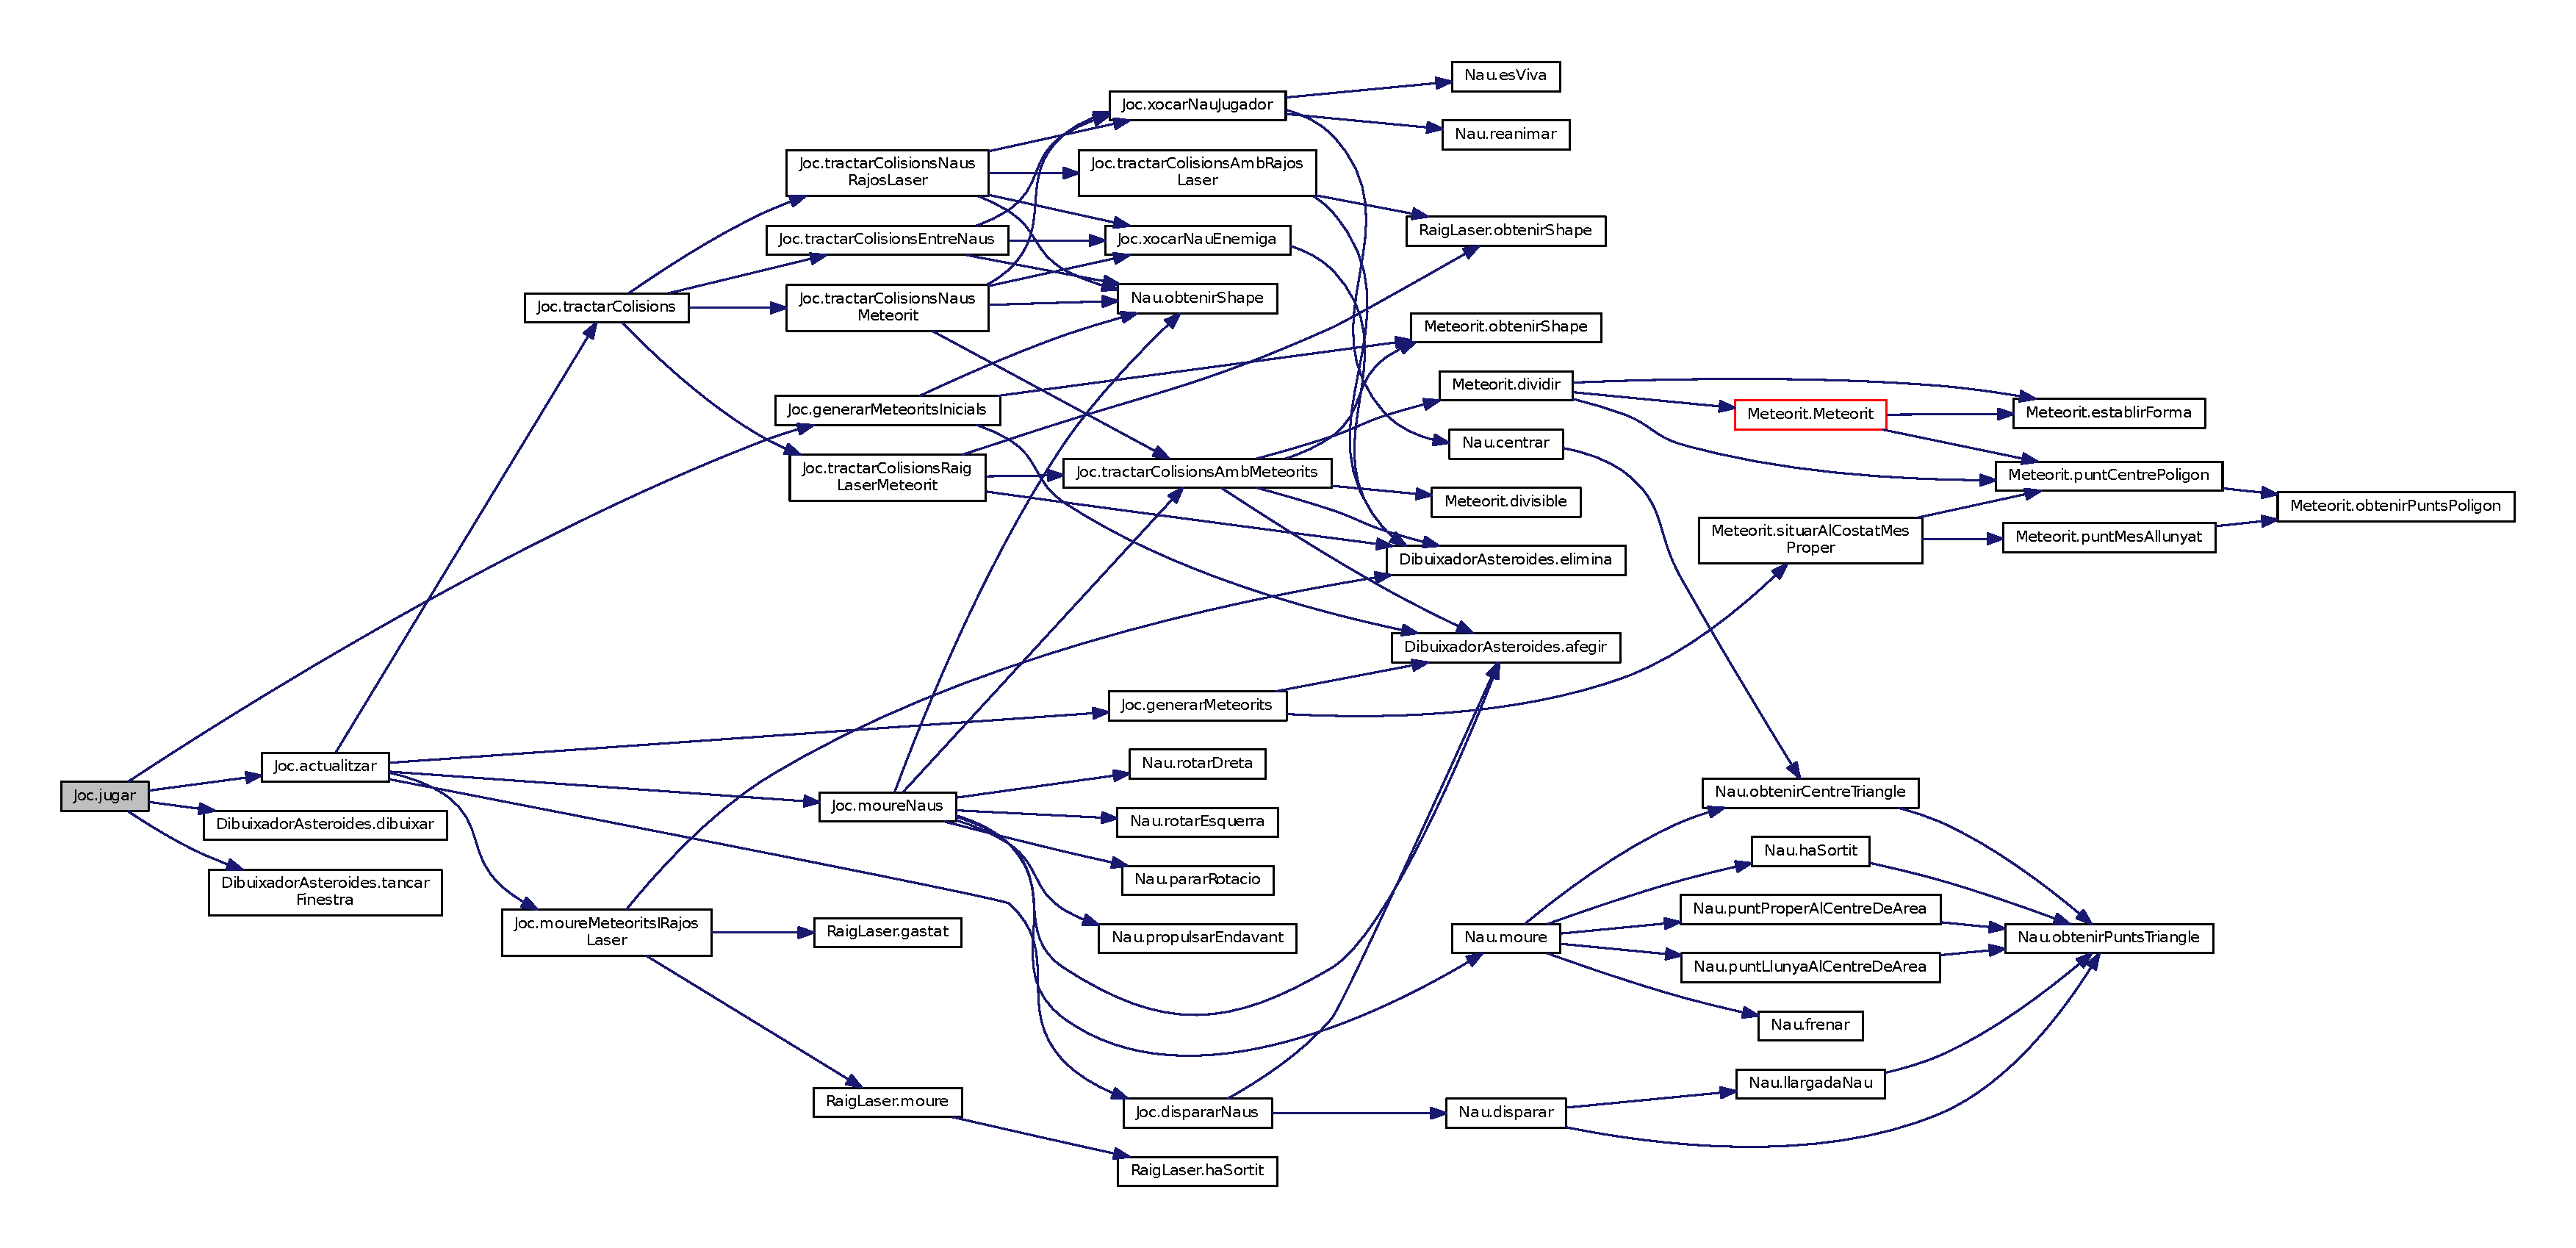
\includegraphics[width=350pt]{class_joc_aa5da4464cac2dc81f26430ac16fa7029_cgraph}
\end{center}
\end{figure}




Here is the caller graph for this function\+:\nopagebreak
\begin{figure}[H]
\begin{center}
\leavevmode
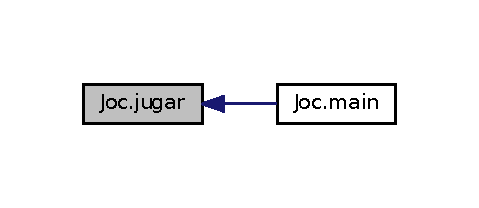
\includegraphics[width=230pt]{class_joc_aa5da4464cac2dc81f26430ac16fa7029_icgraph}
\end{center}
\end{figure}


\hypertarget{class_joc_a54cbe41c97ce7489f7b0cc62217a7d29}{}\index{Joc@{Joc}!main@{main}}
\index{main@{main}!Joc@{Joc}}
\subsubsection[{main}]{\setlength{\rightskip}{0pt plus 5cm}static void Joc.\+main (
\begin{DoxyParamCaption}
\item[{String\mbox{[}$\,$\mbox{]}}]{args}
\end{DoxyParamCaption}
) throws Exception\hspace{0.3cm}{\ttfamily [static]}}\label{class_joc_a54cbe41c97ce7489f7b0cc62217a7d29}


Definition at line 161 of file Joc.\+java.



Here is the call graph for this function\+:\nopagebreak
\begin{figure}[H]
\begin{center}
\leavevmode
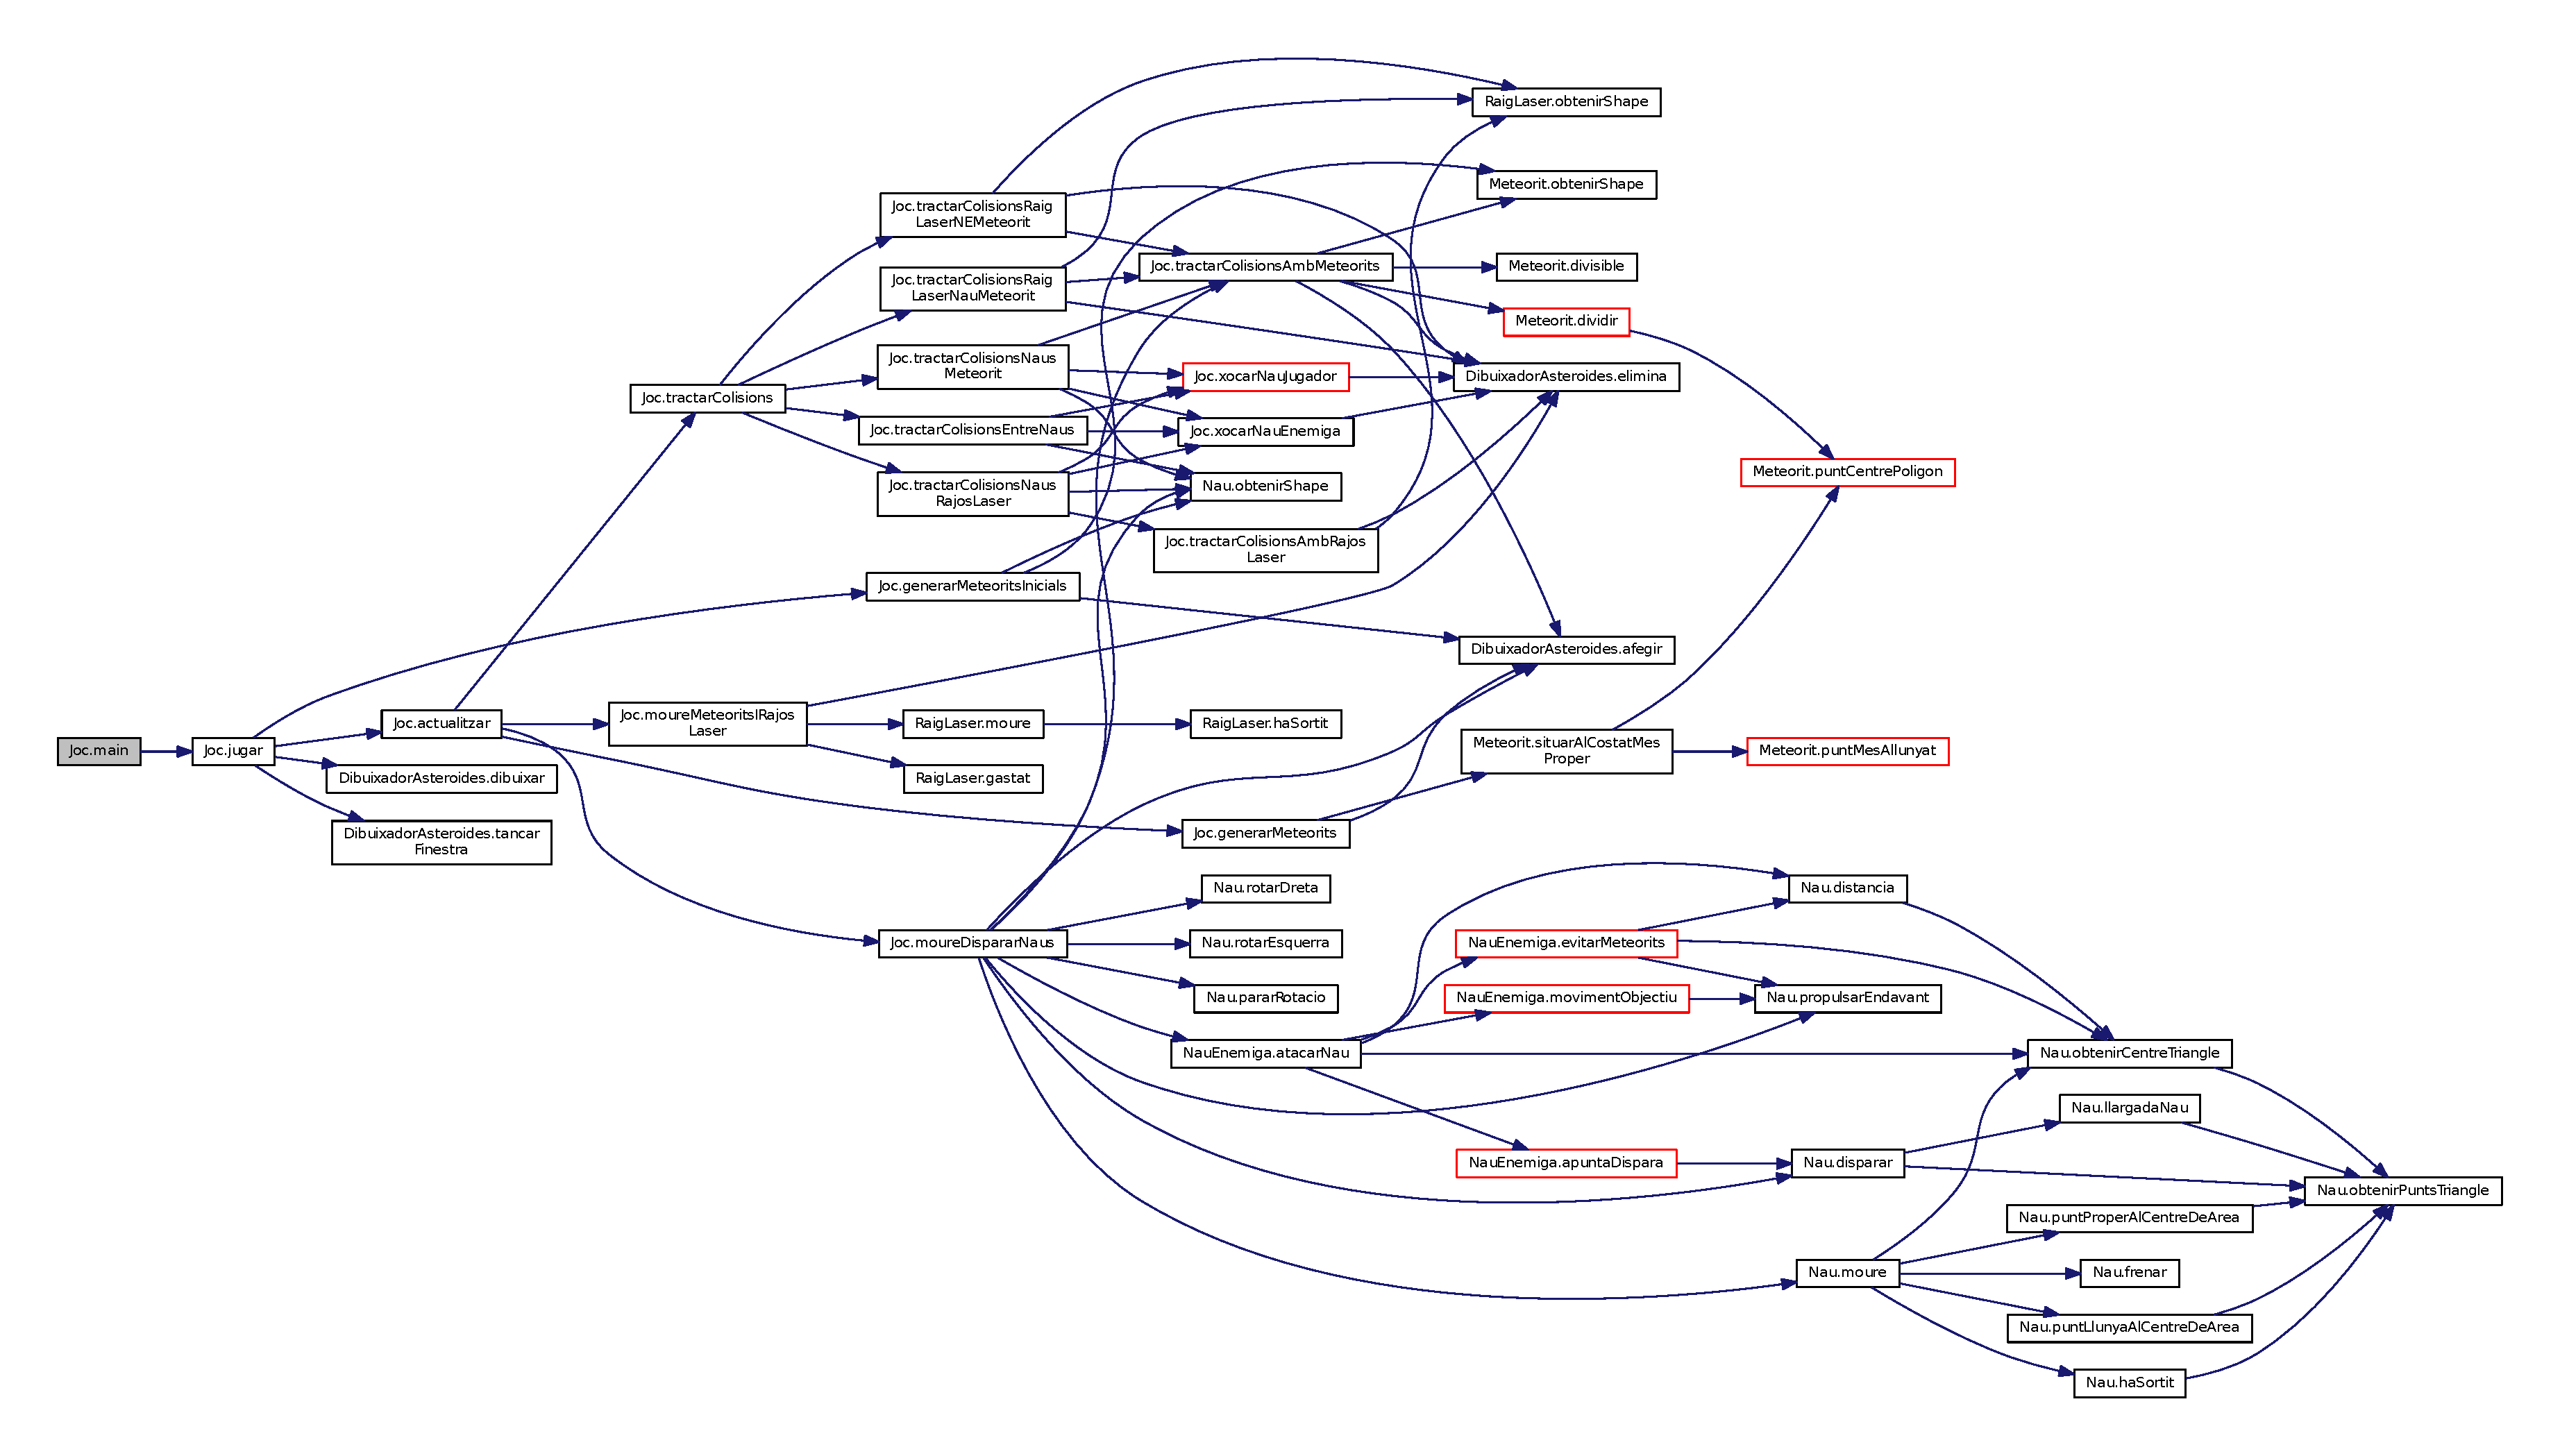
\includegraphics[width=350pt]{class_joc_a54cbe41c97ce7489f7b0cc62217a7d29_cgraph}
\end{center}
\end{figure}


\hypertarget{class_joc_af9e0ddcc5b82db8ff4d07bbd443c7f8d}{}\index{Joc@{Joc}!moure\+Meteorits\+I\+Rajos\+Laser@{moure\+Meteorits\+I\+Rajos\+Laser}}
\index{moure\+Meteorits\+I\+Rajos\+Laser@{moure\+Meteorits\+I\+Rajos\+Laser}!Joc@{Joc}}
\subsubsection[{moure\+Meteorits\+I\+Rajos\+Laser}]{\setlength{\rightskip}{0pt plus 5cm}void Joc.\+moure\+Meteorits\+I\+Rajos\+Laser (
\begin{DoxyParamCaption}
{}
\end{DoxyParamCaption}
) throws Exception\hspace{0.3cm}{\ttfamily [private]}}\label{class_joc_af9e0ddcc5b82db8ff4d07bbd443c7f8d}
\begin{DoxyPrecond}{Precondition}
-- 
\end{DoxyPrecond}
\begin{DoxyPostcond}{Postcondition}
mou els Meteorits i els Rajos\+Laser del \hyperlink{class_joc}{Joc} 
\end{DoxyPostcond}


Definition at line 332 of file Joc.\+java.



Here is the call graph for this function\+:\nopagebreak
\begin{figure}[H]
\begin{center}
\leavevmode
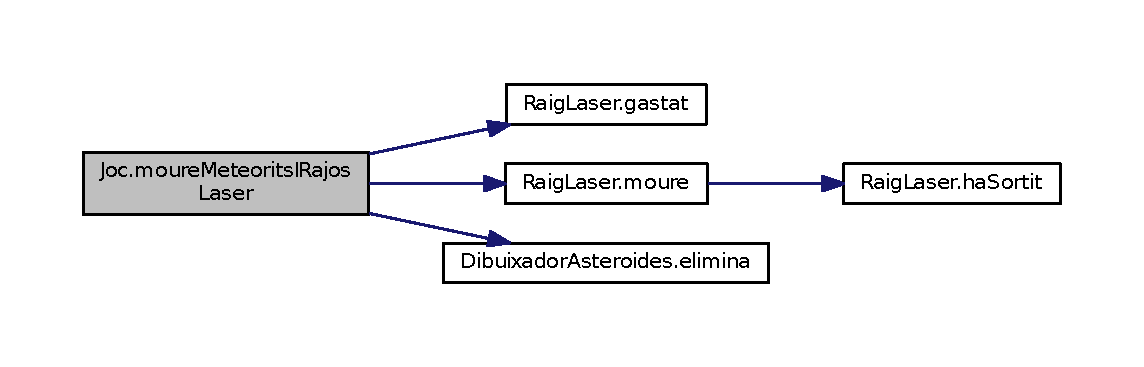
\includegraphics[width=350pt]{class_joc_af9e0ddcc5b82db8ff4d07bbd443c7f8d_cgraph}
\end{center}
\end{figure}




Here is the caller graph for this function\+:\nopagebreak
\begin{figure}[H]
\begin{center}
\leavevmode
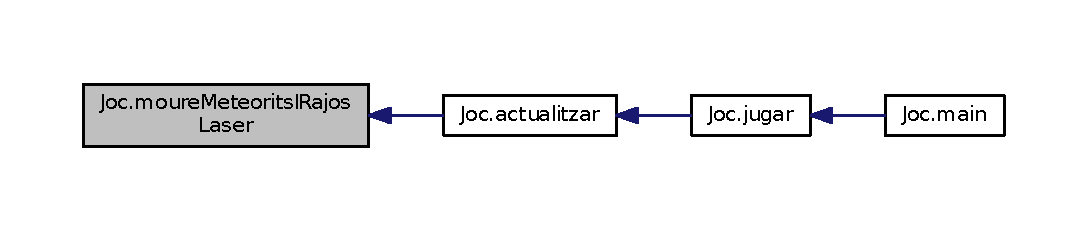
\includegraphics[width=350pt]{class_joc_af9e0ddcc5b82db8ff4d07bbd443c7f8d_icgraph}
\end{center}
\end{figure}


\hypertarget{class_joc_a9b0d8fa2d2613d958dc8bf650ae78a34}{}\index{Joc@{Joc}!moure\+Naus@{moure\+Naus}}
\index{moure\+Naus@{moure\+Naus}!Joc@{Joc}}
\subsubsection[{moure\+Naus}]{\setlength{\rightskip}{0pt plus 5cm}void Joc.\+moure\+Naus (
\begin{DoxyParamCaption}
{}
\end{DoxyParamCaption}
) throws Exception\hspace{0.3cm}{\ttfamily [private]}}\label{class_joc_a9b0d8fa2d2613d958dc8bf650ae78a34}
\begin{DoxyPrecond}{Precondition}
-- 
\end{DoxyPrecond}
\begin{DoxyPostcond}{Postcondition}
mou les Naus del \hyperlink{class_joc}{Joc} 
\end{DoxyPostcond}


Definition at line 299 of file Joc.\+java.



Here is the call graph for this function\+:\nopagebreak
\begin{figure}[H]
\begin{center}
\leavevmode
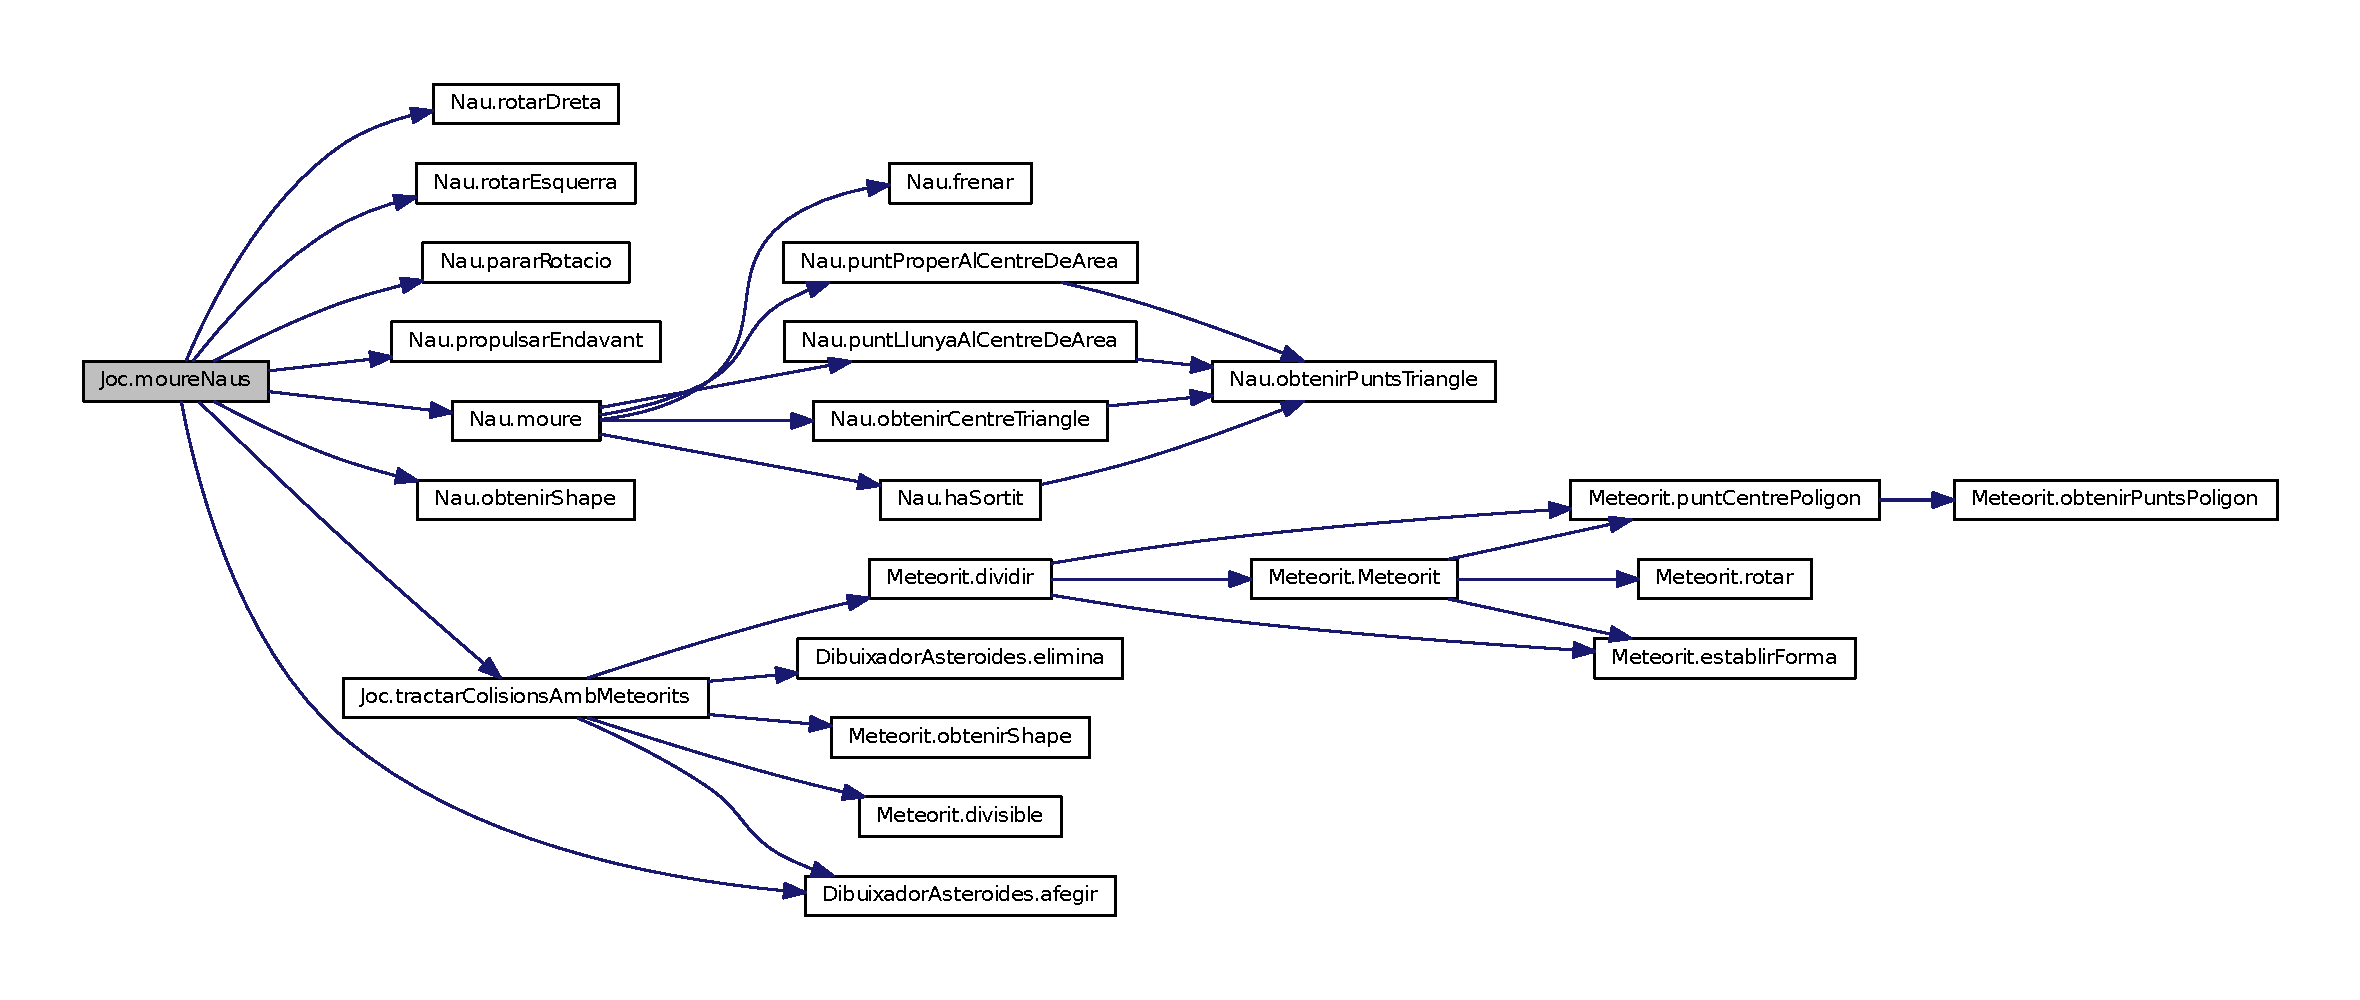
\includegraphics[width=350pt]{class_joc_a9b0d8fa2d2613d958dc8bf650ae78a34_cgraph}
\end{center}
\end{figure}




Here is the caller graph for this function\+:\nopagebreak
\begin{figure}[H]
\begin{center}
\leavevmode
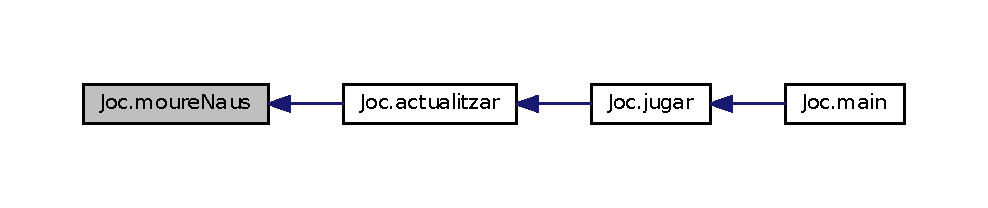
\includegraphics[width=350pt]{class_joc_a9b0d8fa2d2613d958dc8bf650ae78a34_icgraph}
\end{center}
\end{figure}


\hypertarget{class_joc_a1be330c10f1e2ee06f696e0a0bdec7c7}{}\index{Joc@{Joc}!tractar\+Colisions@{tractar\+Colisions}}
\index{tractar\+Colisions@{tractar\+Colisions}!Joc@{Joc}}
\subsubsection[{tractar\+Colisions}]{\setlength{\rightskip}{0pt plus 5cm}void Joc.\+tractar\+Colisions (
\begin{DoxyParamCaption}
{}
\end{DoxyParamCaption}
) throws Exception\hspace{0.3cm}{\ttfamily [private]}}\label{class_joc_a1be330c10f1e2ee06f696e0a0bdec7c7}
\begin{DoxyPrecond}{Precondition}
-- 
\end{DoxyPrecond}
\begin{DoxyPostcond}{Postcondition}
tracta les col·lisions entre els objectes del \hyperlink{class_joc}{Joc} 
\end{DoxyPostcond}


Definition at line 363 of file Joc.\+java.



Here is the call graph for this function\+:\nopagebreak
\begin{figure}[H]
\begin{center}
\leavevmode
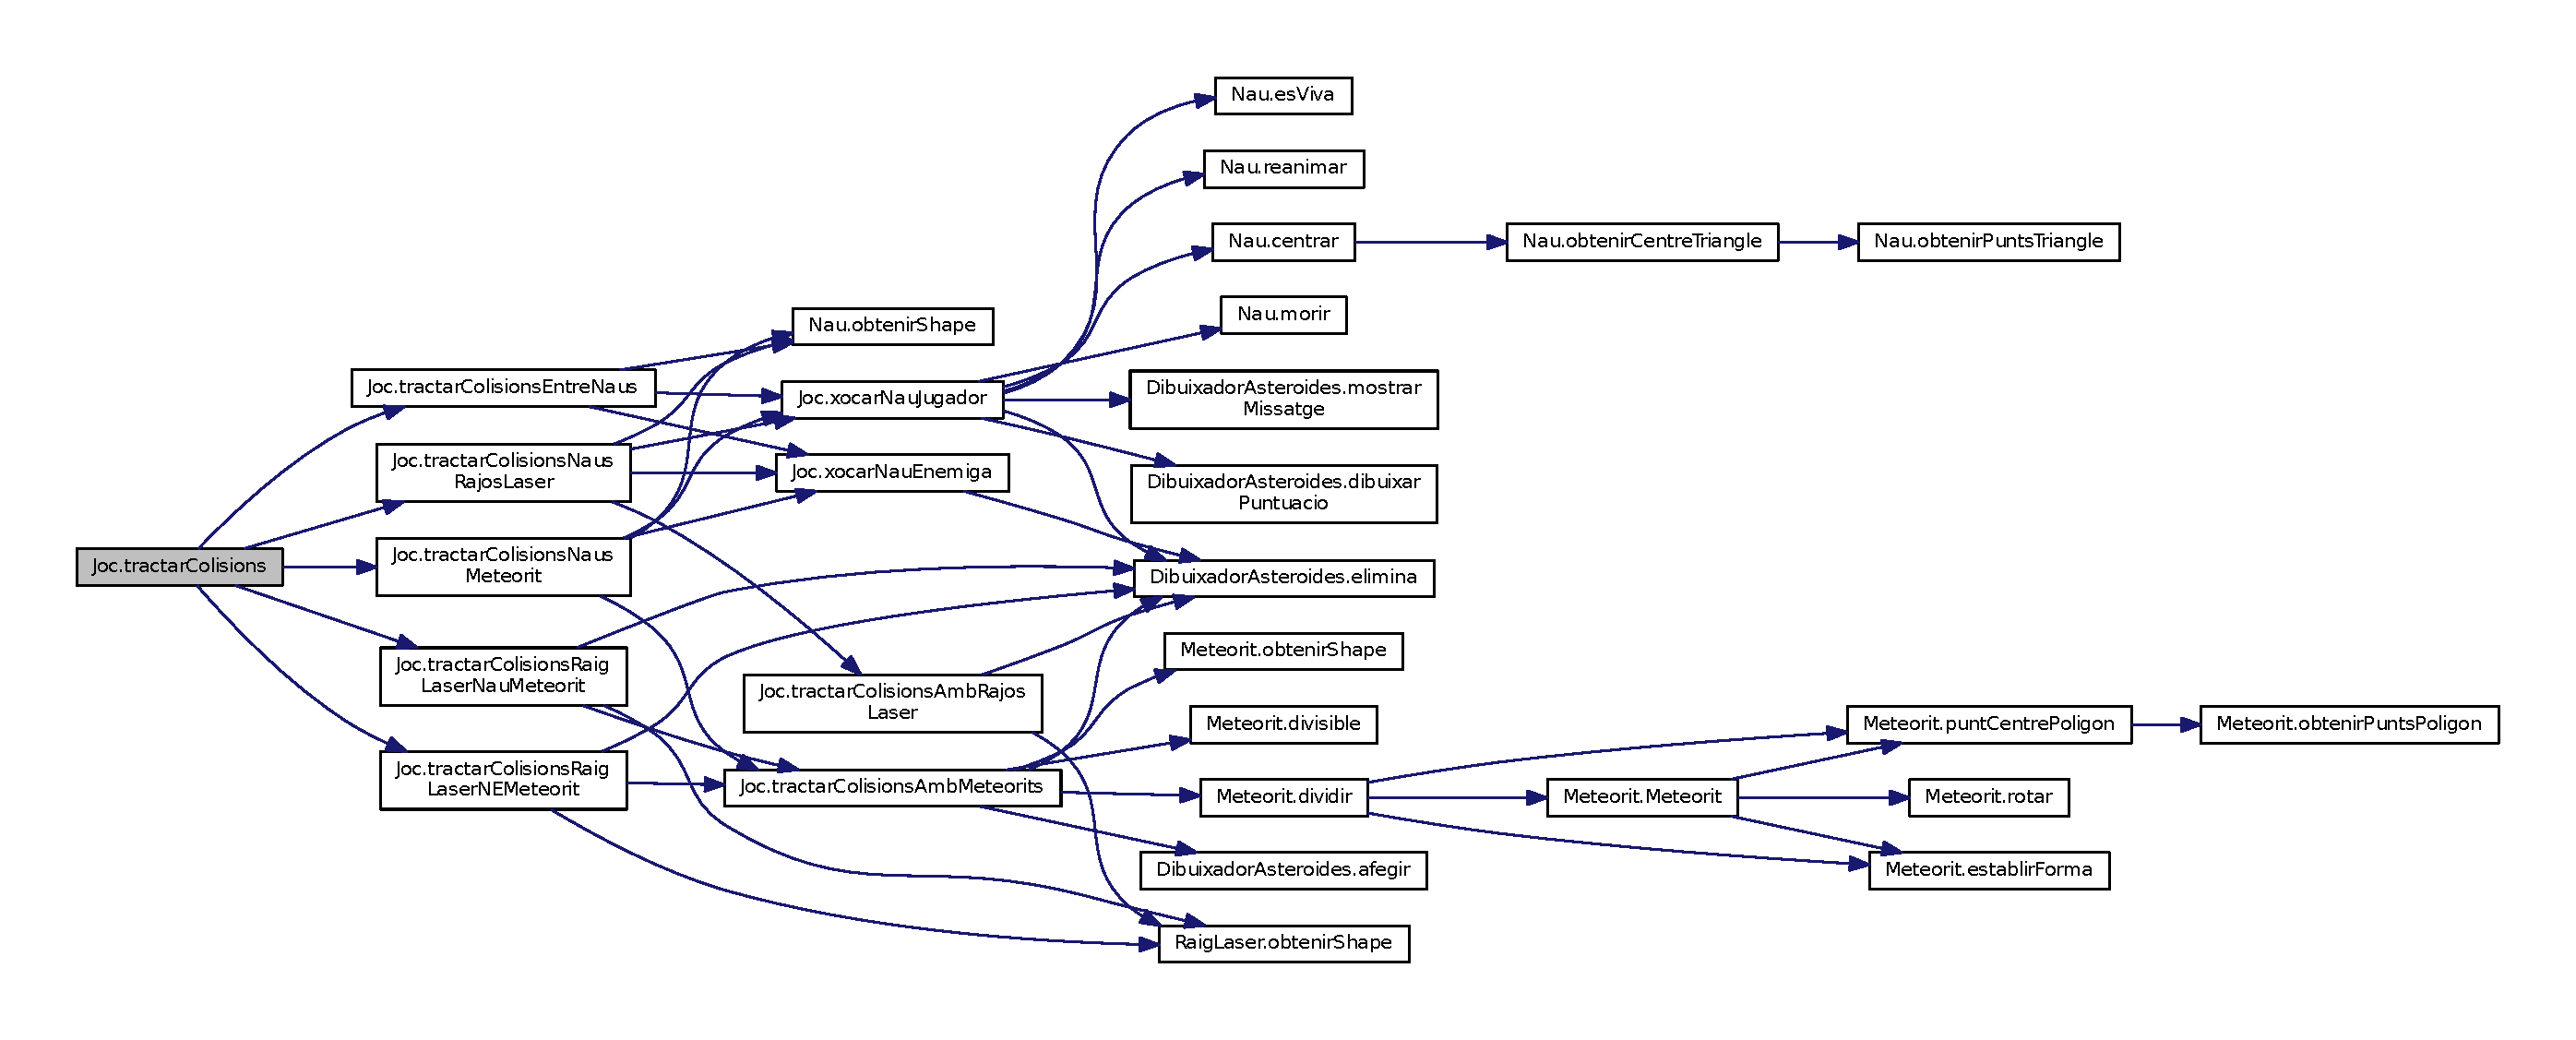
\includegraphics[width=350pt]{class_joc_a1be330c10f1e2ee06f696e0a0bdec7c7_cgraph}
\end{center}
\end{figure}




Here is the caller graph for this function\+:\nopagebreak
\begin{figure}[H]
\begin{center}
\leavevmode
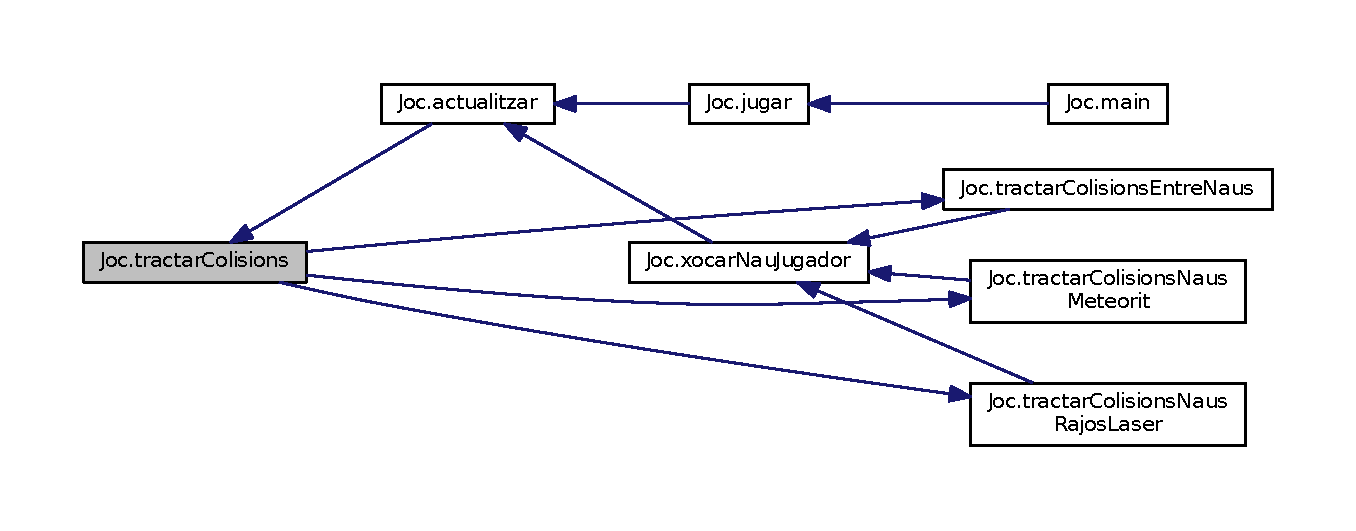
\includegraphics[width=350pt]{class_joc_a1be330c10f1e2ee06f696e0a0bdec7c7_icgraph}
\end{center}
\end{figure}


\hypertarget{class_joc_a16b0be1ee6298106946df8150044f667}{}\index{Joc@{Joc}!tractar\+Colisions\+Amb\+Meteorits@{tractar\+Colisions\+Amb\+Meteorits}}
\index{tractar\+Colisions\+Amb\+Meteorits@{tractar\+Colisions\+Amb\+Meteorits}!Joc@{Joc}}
\subsubsection[{tractar\+Colisions\+Amb\+Meteorits}]{\setlength{\rightskip}{0pt plus 5cm}boolean Joc.\+tractar\+Colisions\+Amb\+Meteorits (
\begin{DoxyParamCaption}
\item[{Area}]{a, }
\item[{boolean}]{puntuar}
\end{DoxyParamCaption}
) throws Exception\hspace{0.3cm}{\ttfamily [private]}}\label{class_joc_a16b0be1ee6298106946df8150044f667}
\begin{DoxyPrecond}{Precondition}
-- 
\end{DoxyPrecond}
\begin{DoxyPostcond}{Postcondition}
retorna si l\textquotesingle{}Area a ha colisionat amb algun \hyperlink{class_meteorit}{Meteorit} i actualitza la puntuació 
\end{DoxyPostcond}


Definition at line 472 of file Joc.\+java.



Here is the call graph for this function\+:\nopagebreak
\begin{figure}[H]
\begin{center}
\leavevmode
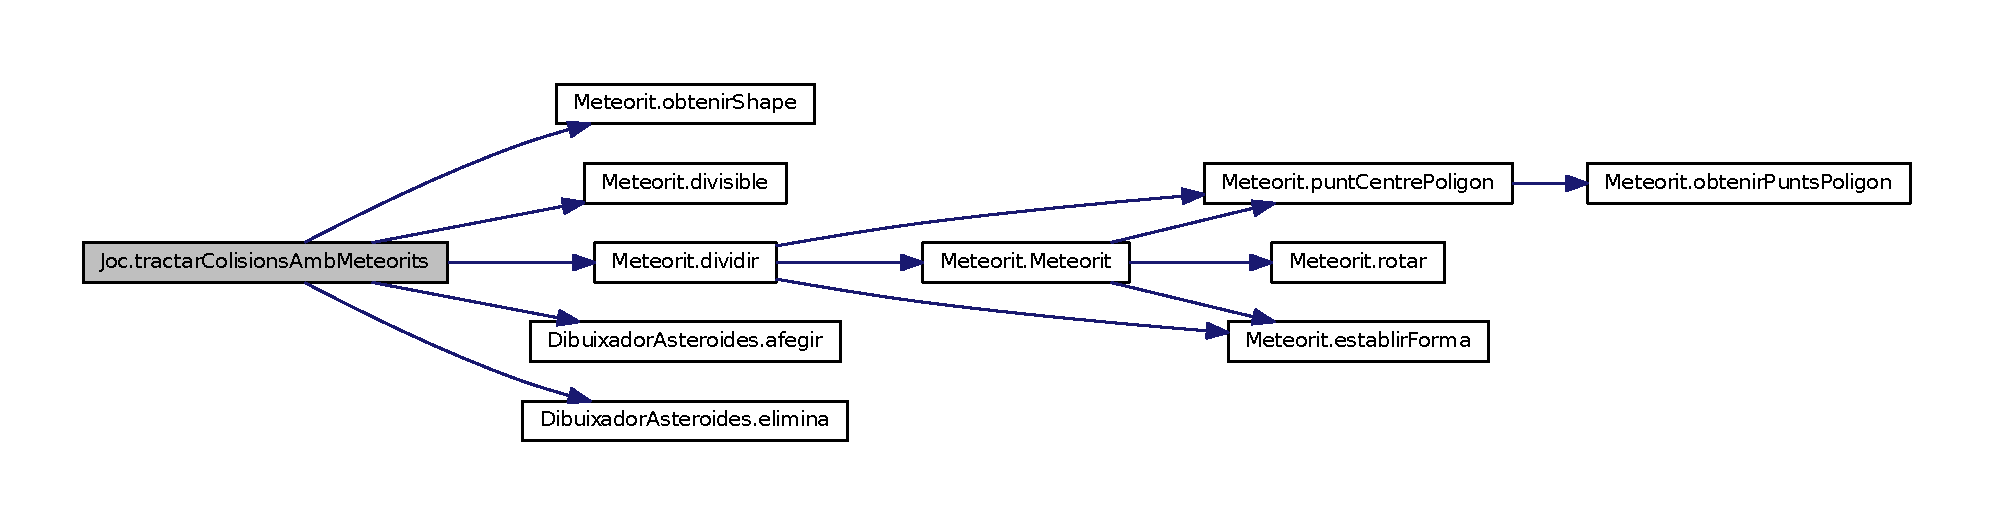
\includegraphics[width=350pt]{class_joc_a16b0be1ee6298106946df8150044f667_cgraph}
\end{center}
\end{figure}




Here is the caller graph for this function\+:\nopagebreak
\begin{figure}[H]
\begin{center}
\leavevmode
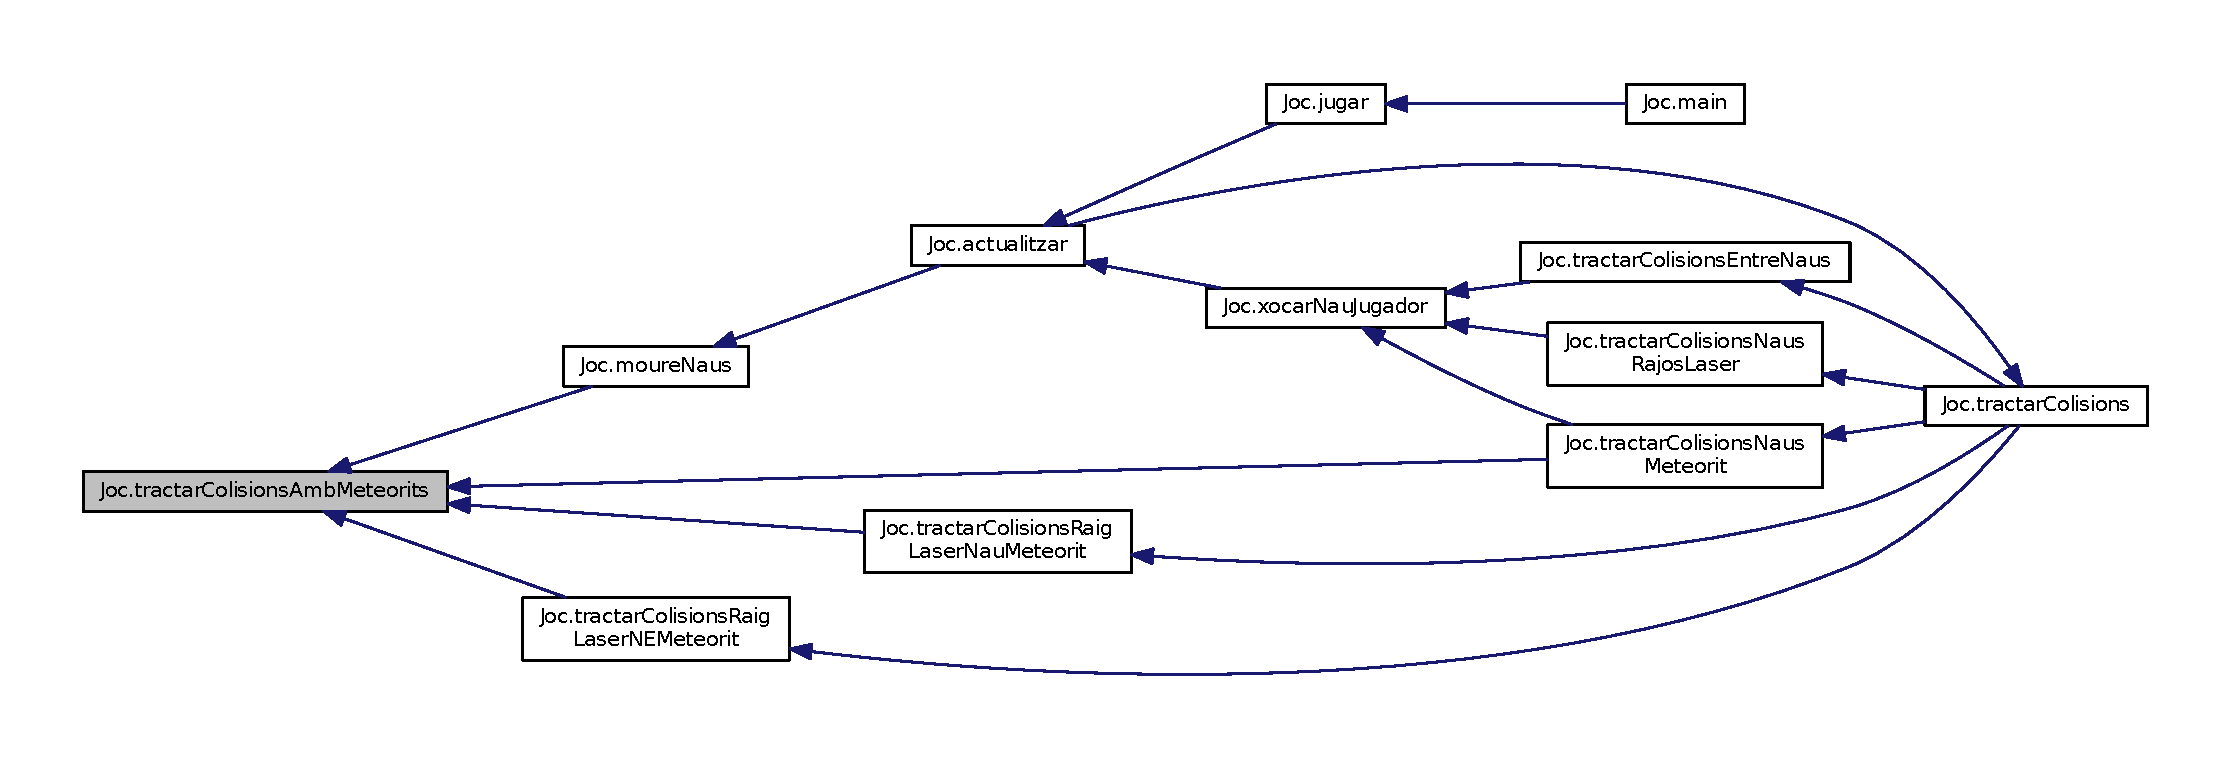
\includegraphics[width=350pt]{class_joc_a16b0be1ee6298106946df8150044f667_icgraph}
\end{center}
\end{figure}


\hypertarget{class_joc_ac94f4a327797f506171f0db74b3feaee}{}\index{Joc@{Joc}!tractar\+Colisions\+Amb\+Rajos\+Laser@{tractar\+Colisions\+Amb\+Rajos\+Laser}}
\index{tractar\+Colisions\+Amb\+Rajos\+Laser@{tractar\+Colisions\+Amb\+Rajos\+Laser}!Joc@{Joc}}
\subsubsection[{tractar\+Colisions\+Amb\+Rajos\+Laser}]{\setlength{\rightskip}{0pt plus 5cm}boolean Joc.\+tractar\+Colisions\+Amb\+Rajos\+Laser (
\begin{DoxyParamCaption}
\item[{Area}]{a}
\end{DoxyParamCaption}
) throws Exception\hspace{0.3cm}{\ttfamily [private]}}\label{class_joc_ac94f4a327797f506171f0db74b3feaee}
\begin{DoxyPrecond}{Precondition}
-- 
\end{DoxyPrecond}
\begin{DoxyPostcond}{Postcondition}
si a ha xocat amb algun \hyperlink{class_raig_laser}{Raig\+Laser}, retorna cert i elimina el \hyperlink{class_raig_laser}{Raig\+Laser}, altrament retorna fals 
\end{DoxyPostcond}


Definition at line 543 of file Joc.\+java.



Here is the call graph for this function\+:\nopagebreak
\begin{figure}[H]
\begin{center}
\leavevmode
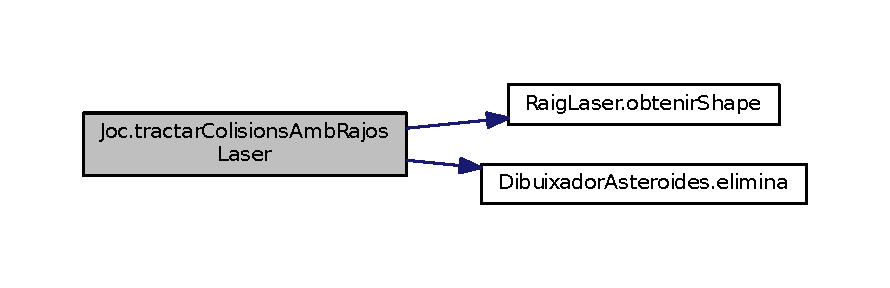
\includegraphics[width=350pt]{class_joc_ac94f4a327797f506171f0db74b3feaee_cgraph}
\end{center}
\end{figure}




Here is the caller graph for this function\+:\nopagebreak
\begin{figure}[H]
\begin{center}
\leavevmode
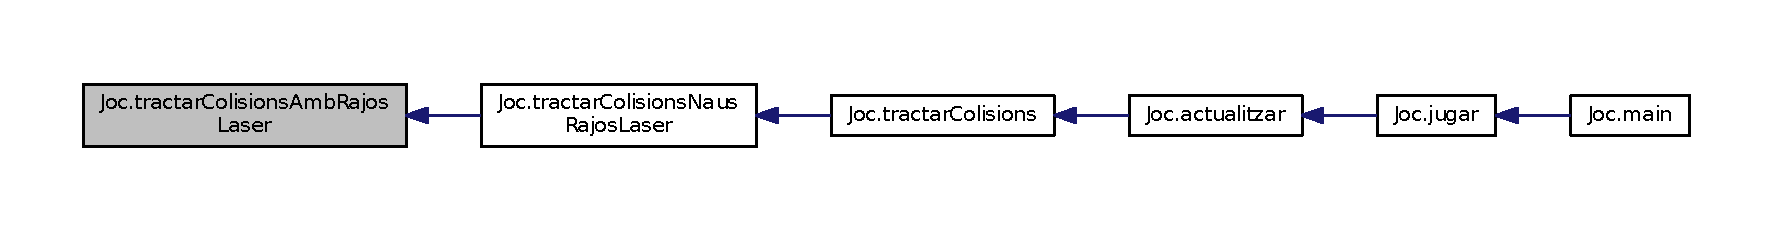
\includegraphics[width=350pt]{class_joc_ac94f4a327797f506171f0db74b3feaee_icgraph}
\end{center}
\end{figure}


\hypertarget{class_joc_abc5db47ede50ddeccb50b2872d05cb6c}{}\index{Joc@{Joc}!tractar\+Colisions\+Entre\+Naus@{tractar\+Colisions\+Entre\+Naus}}
\index{tractar\+Colisions\+Entre\+Naus@{tractar\+Colisions\+Entre\+Naus}!Joc@{Joc}}
\subsubsection[{tractar\+Colisions\+Entre\+Naus}]{\setlength{\rightskip}{0pt plus 5cm}void Joc.\+tractar\+Colisions\+Entre\+Naus (
\begin{DoxyParamCaption}
{}
\end{DoxyParamCaption}
) throws Exception\hspace{0.3cm}{\ttfamily [private]}}\label{class_joc_abc5db47ede50ddeccb50b2872d05cb6c}
\begin{DoxyPrecond}{Precondition}
-- 
\end{DoxyPrecond}
\begin{DoxyPostcond}{Postcondition}
si les naus colisionen la \hyperlink{class_nau}{Nau} del jugador es centra, la \hyperlink{class_nau_enemiga}{Nau\+Enemiga} desapareix durant 5 segons i s\textquotesingle{}actualitza la puntuació, altrament no fa res 
\end{DoxyPostcond}


Definition at line 423 of file Joc.\+java.



Here is the call graph for this function\+:\nopagebreak
\begin{figure}[H]
\begin{center}
\leavevmode
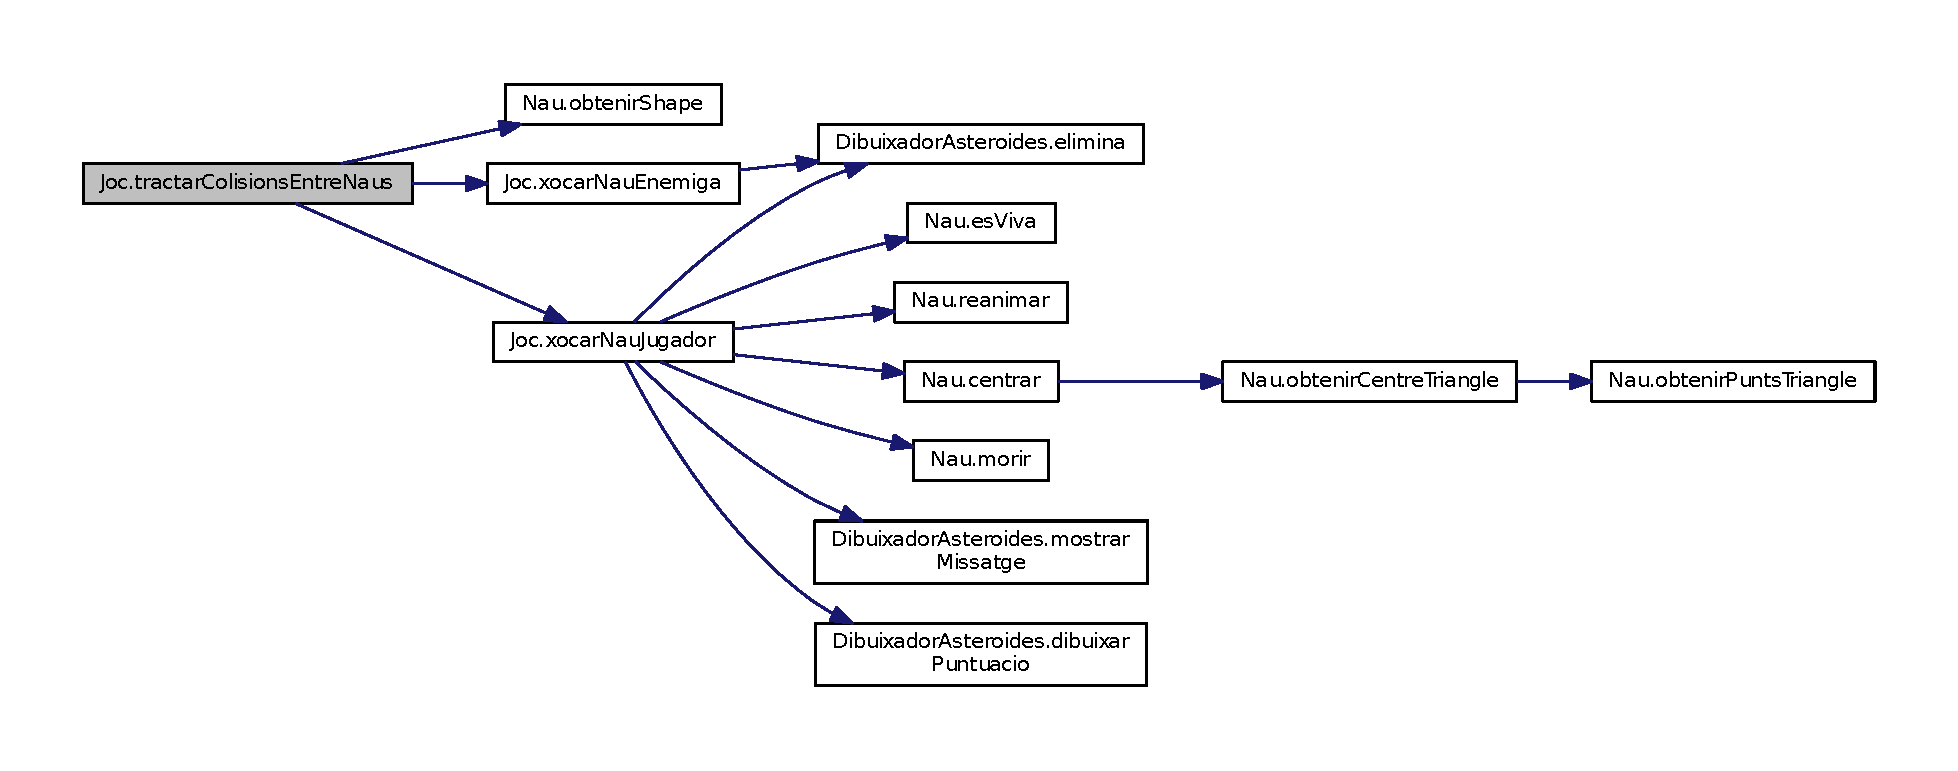
\includegraphics[width=350pt]{class_joc_abc5db47ede50ddeccb50b2872d05cb6c_cgraph}
\end{center}
\end{figure}




Here is the caller graph for this function\+:\nopagebreak
\begin{figure}[H]
\begin{center}
\leavevmode
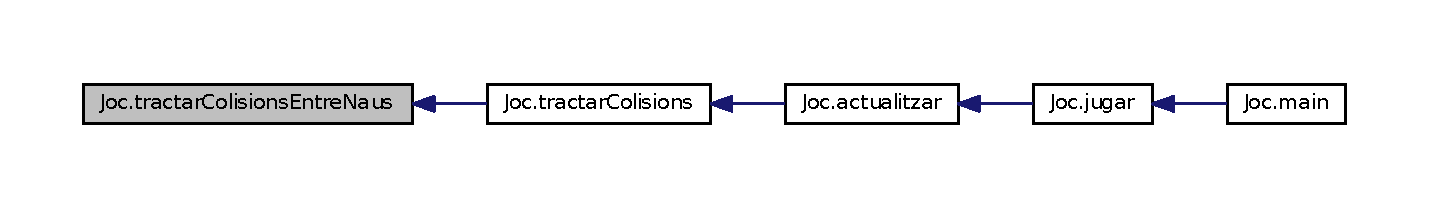
\includegraphics[width=350pt]{class_joc_abc5db47ede50ddeccb50b2872d05cb6c_icgraph}
\end{center}
\end{figure}


\hypertarget{class_joc_acf31c665e8f734f15f40f8e6792e8bba}{}\index{Joc@{Joc}!tractar\+Colisions\+Naus\+Meteorit@{tractar\+Colisions\+Naus\+Meteorit}}
\index{tractar\+Colisions\+Naus\+Meteorit@{tractar\+Colisions\+Naus\+Meteorit}!Joc@{Joc}}
\subsubsection[{tractar\+Colisions\+Naus\+Meteorit}]{\setlength{\rightskip}{0pt plus 5cm}void Joc.\+tractar\+Colisions\+Naus\+Meteorit (
\begin{DoxyParamCaption}
{}
\end{DoxyParamCaption}
) throws Exception\hspace{0.3cm}{\ttfamily [private]}}\label{class_joc_acf31c665e8f734f15f40f8e6792e8bba}
\begin{DoxyPrecond}{Precondition}
-- 
\end{DoxyPrecond}
\begin{DoxyPostcond}{Postcondition}
si la \hyperlink{class_nau}{Nau} del jugador ha xocat amb algun \hyperlink{class_meteorit}{Meteorit}, aquesta es centra i perd una vida, i el \hyperlink{class_meteorit}{Meteorit} es divideix o desapareix segons la mida si la \hyperlink{class_nau_enemiga}{Nau\+Enemiga} ha xocat amb algun \hyperlink{class_meteorit}{Meteorit}, aquesta es canvia de lloc aleatòriament i el \hyperlink{class_meteorit}{Meteorit} es divideix o desapareix segons la mida 
\end{DoxyPostcond}


Definition at line 507 of file Joc.\+java.



Here is the call graph for this function\+:\nopagebreak
\begin{figure}[H]
\begin{center}
\leavevmode
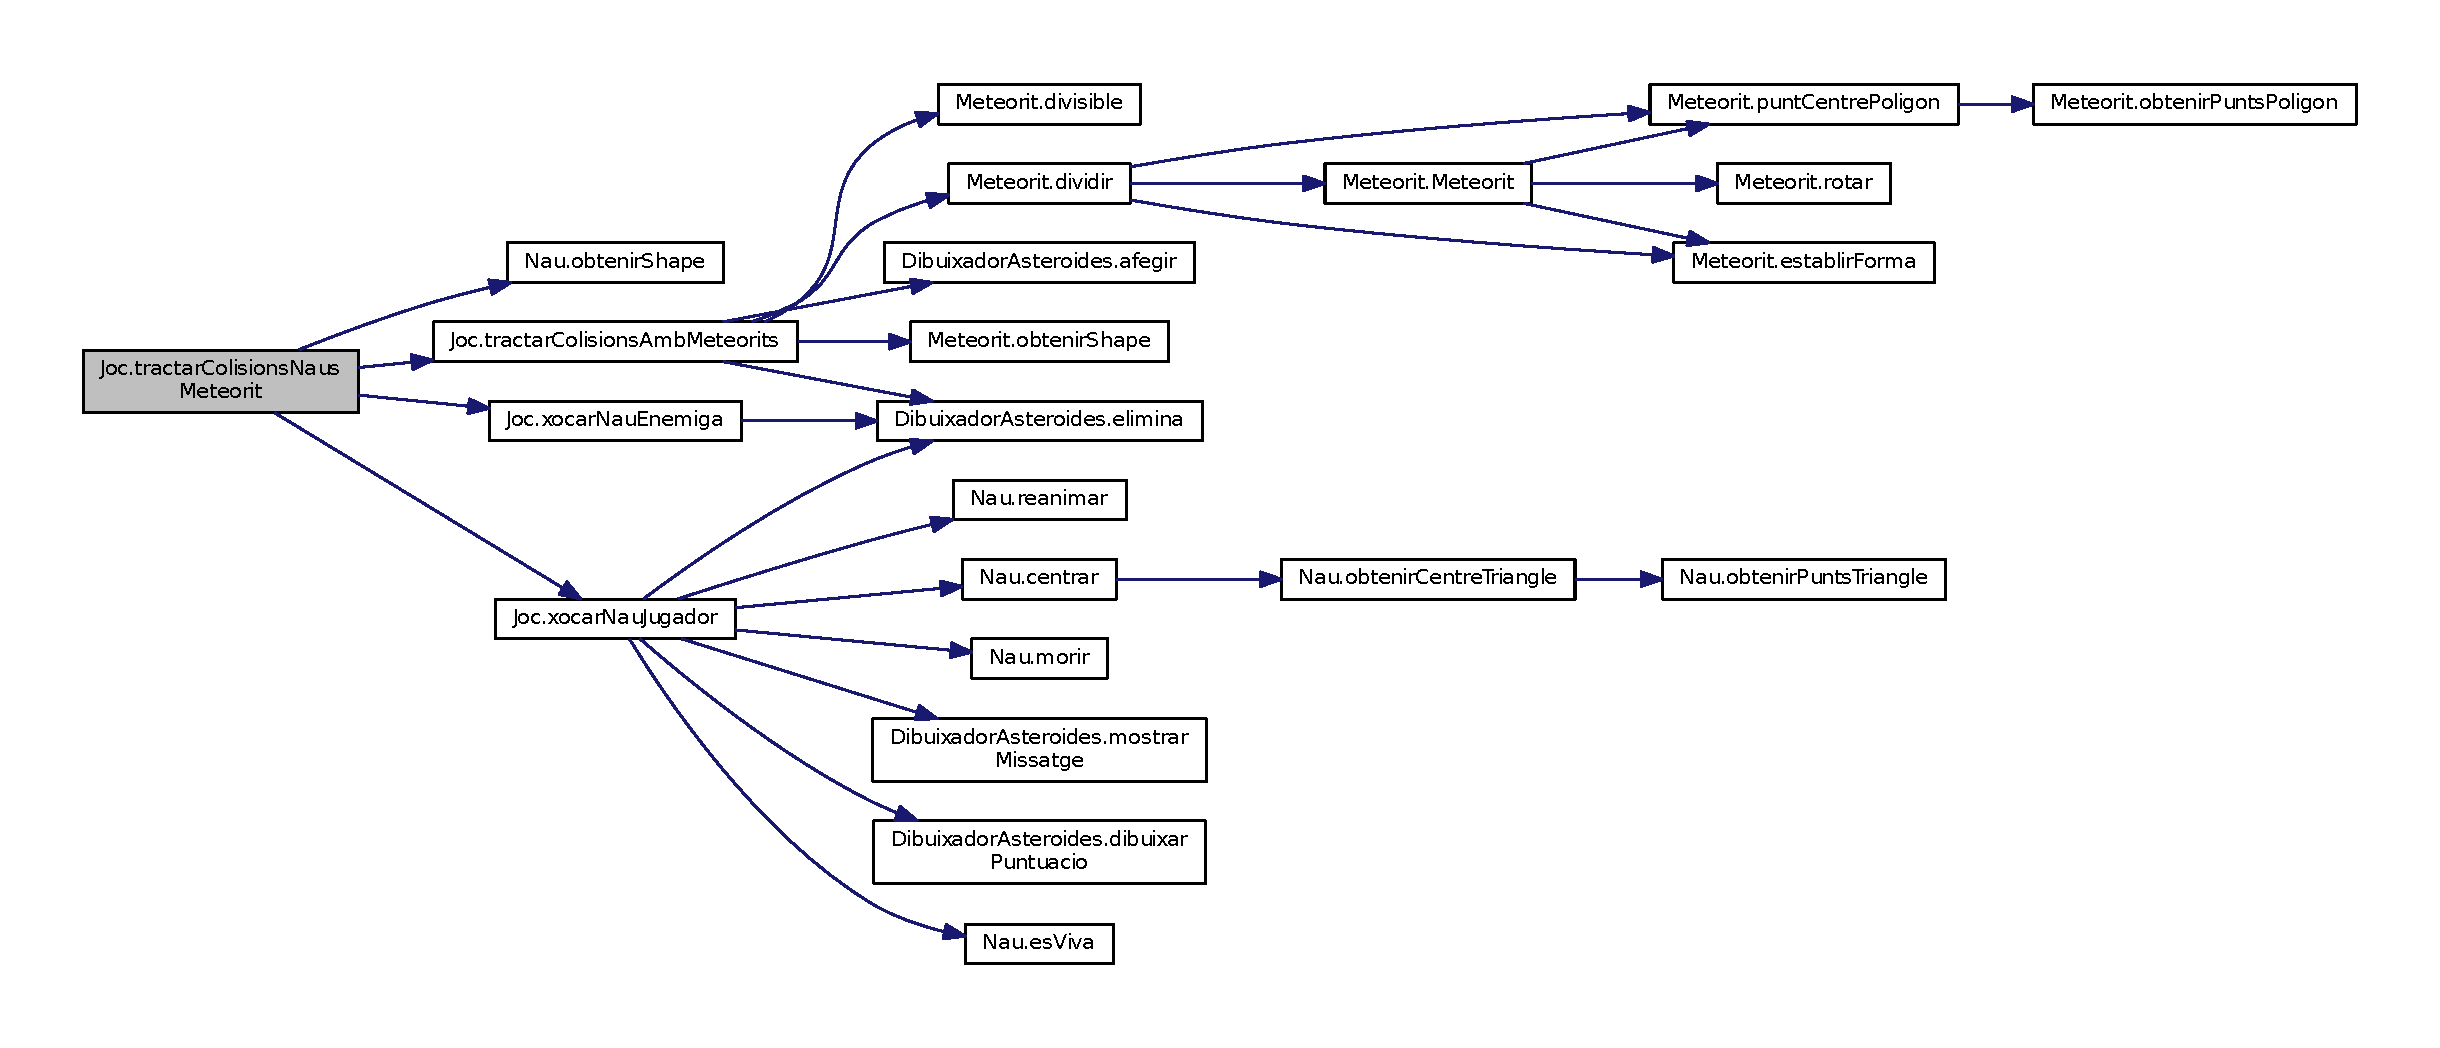
\includegraphics[width=350pt]{class_joc_acf31c665e8f734f15f40f8e6792e8bba_cgraph}
\end{center}
\end{figure}




Here is the caller graph for this function\+:\nopagebreak
\begin{figure}[H]
\begin{center}
\leavevmode
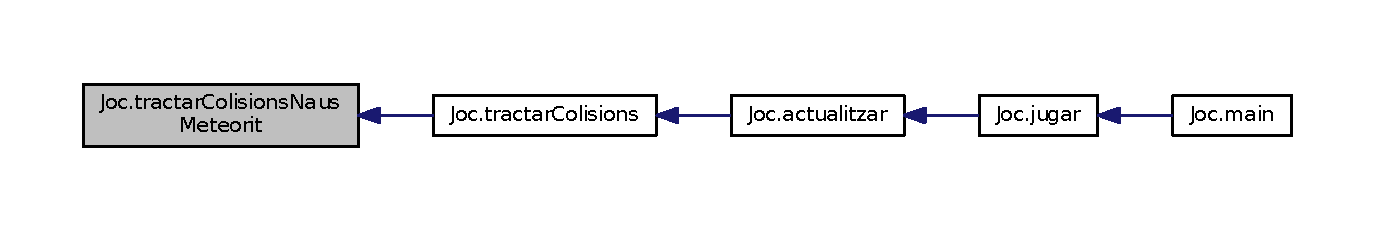
\includegraphics[width=350pt]{class_joc_acf31c665e8f734f15f40f8e6792e8bba_icgraph}
\end{center}
\end{figure}


\hypertarget{class_joc_a9ccc5adec1e7efdd6c01ba393d3686c6}{}\index{Joc@{Joc}!tractar\+Colisions\+Naus\+Rajos\+Laser@{tractar\+Colisions\+Naus\+Rajos\+Laser}}
\index{tractar\+Colisions\+Naus\+Rajos\+Laser@{tractar\+Colisions\+Naus\+Rajos\+Laser}!Joc@{Joc}}
\subsubsection[{tractar\+Colisions\+Naus\+Rajos\+Laser}]{\setlength{\rightskip}{0pt plus 5cm}void Joc.\+tractar\+Colisions\+Naus\+Rajos\+Laser (
\begin{DoxyParamCaption}
{}
\end{DoxyParamCaption}
) throws Exception\hspace{0.3cm}{\ttfamily [private]}}\label{class_joc_a9ccc5adec1e7efdd6c01ba393d3686c6}
\begin{DoxyPrecond}{Precondition}
-- 
\end{DoxyPrecond}
\begin{DoxyPostcond}{Postcondition}
si la \hyperlink{class_nau}{Nau} del jugador ha xocat amb algun \hyperlink{class_raig_laser}{Raig\+Laser}, aquesta es centra i perd una vida, i el \hyperlink{class_raig_laser}{Raig\+Laser} desapareix si la \hyperlink{class_nau_enemiga}{Nau\+Enemiga} ha xocat amb algun \hyperlink{class_raig_laser}{Raig\+Laser}, aquesta desapareix i torna a aparèixer al cap de 10 segons, i el \hyperlink{class_raig_laser}{Raig\+Laser} desapareix 
\end{DoxyPostcond}


Definition at line 526 of file Joc.\+java.



Here is the call graph for this function\+:\nopagebreak
\begin{figure}[H]
\begin{center}
\leavevmode
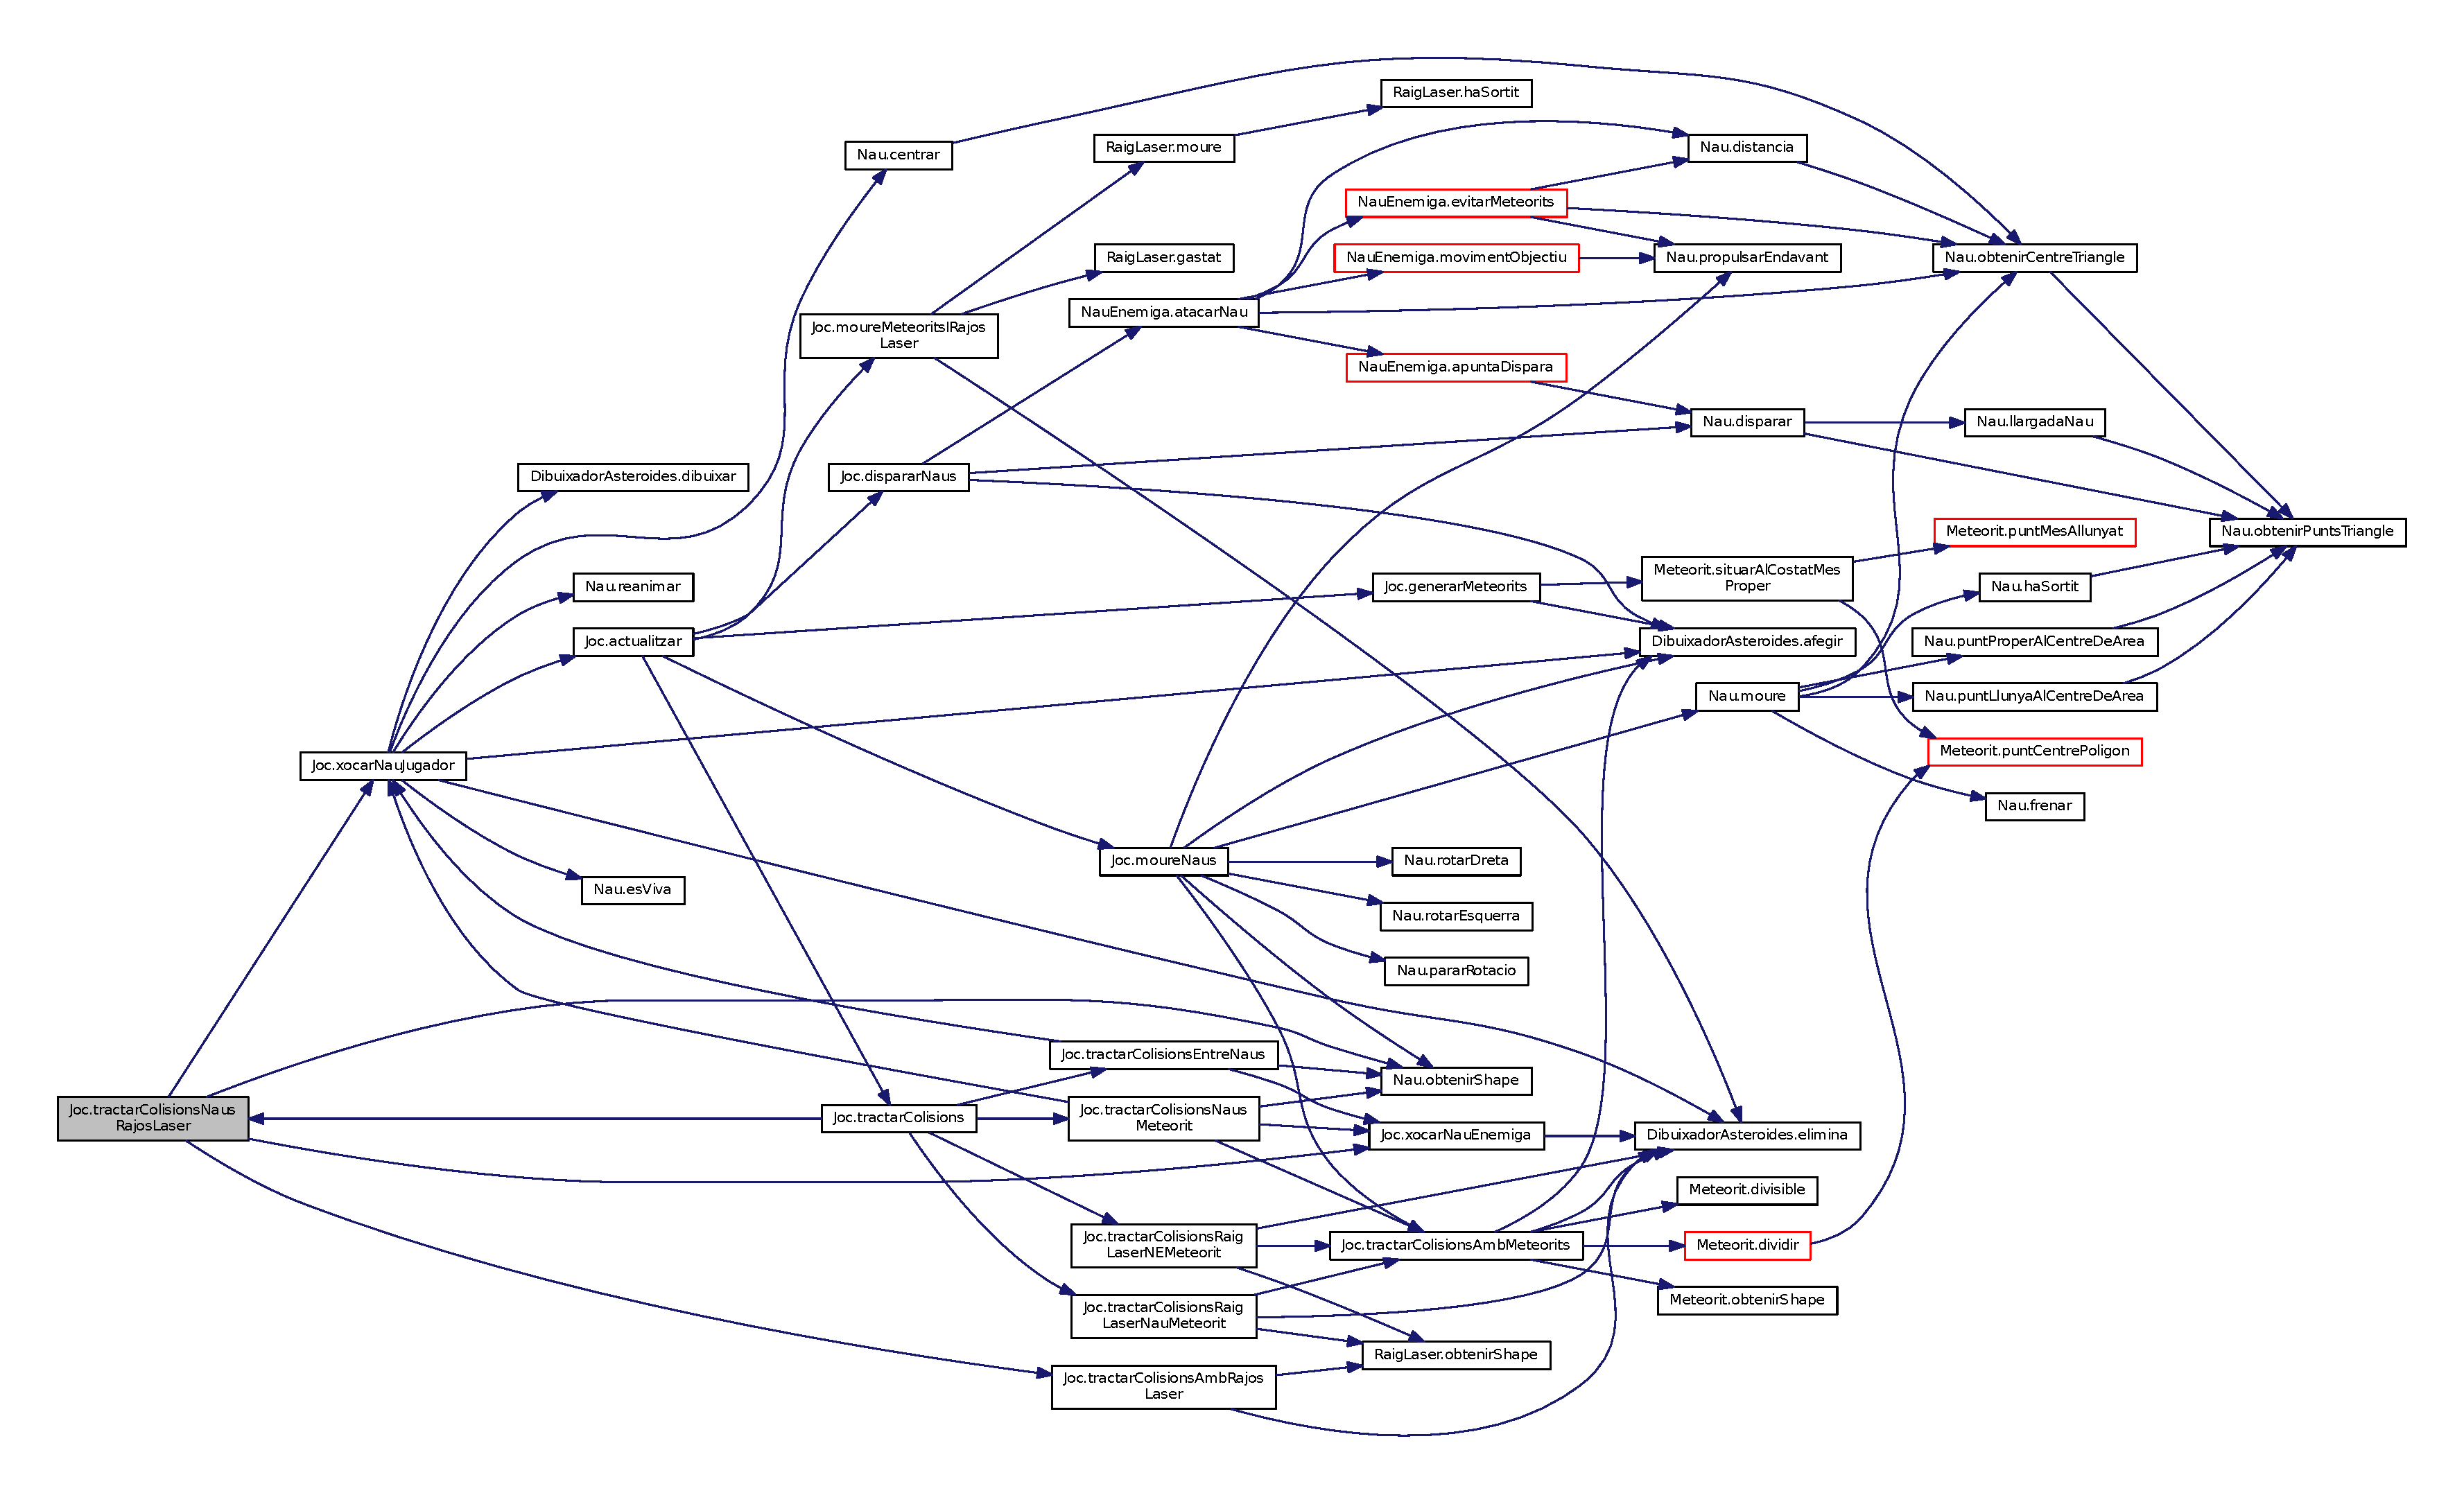
\includegraphics[width=350pt]{class_joc_a9ccc5adec1e7efdd6c01ba393d3686c6_cgraph}
\end{center}
\end{figure}




Here is the caller graph for this function\+:\nopagebreak
\begin{figure}[H]
\begin{center}
\leavevmode
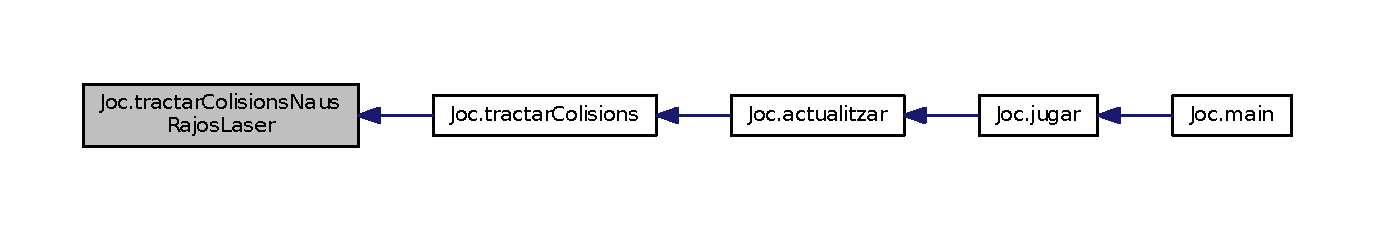
\includegraphics[width=350pt]{class_joc_a9ccc5adec1e7efdd6c01ba393d3686c6_icgraph}
\end{center}
\end{figure}


\hypertarget{class_joc_a9a3116242cc69985726f4825be70a9b5}{}\index{Joc@{Joc}!tractar\+Colisions\+Raig\+Laser\+Nau\+Meteorit@{tractar\+Colisions\+Raig\+Laser\+Nau\+Meteorit}}
\index{tractar\+Colisions\+Raig\+Laser\+Nau\+Meteorit@{tractar\+Colisions\+Raig\+Laser\+Nau\+Meteorit}!Joc@{Joc}}
\subsubsection[{tractar\+Colisions\+Raig\+Laser\+Nau\+Meteorit}]{\setlength{\rightskip}{0pt plus 5cm}void Joc.\+tractar\+Colisions\+Raig\+Laser\+Nau\+Meteorit (
\begin{DoxyParamCaption}
{}
\end{DoxyParamCaption}
) throws Exception\hspace{0.3cm}{\ttfamily [private]}}\label{class_joc_a9a3116242cc69985726f4825be70a9b5}
\begin{DoxyPrecond}{Precondition}
-- 
\end{DoxyPrecond}
\begin{DoxyPostcond}{Postcondition}
els \hyperlink{class_raig_laser}{Raig\+Laser} de la \hyperlink{class_nau}{Nau} que hagin col·lisionat amb un \hyperlink{class_meteorit}{Meteorit} s\textquotesingle{}han eliminat i els Meteorits s\textquotesingle{}han dividit o bé eliminat segons la seva mida, s\textquotesingle{}ha actualitzat la puntuació 
\end{DoxyPostcond}


Definition at line 438 of file Joc.\+java.



Here is the call graph for this function\+:\nopagebreak
\begin{figure}[H]
\begin{center}
\leavevmode
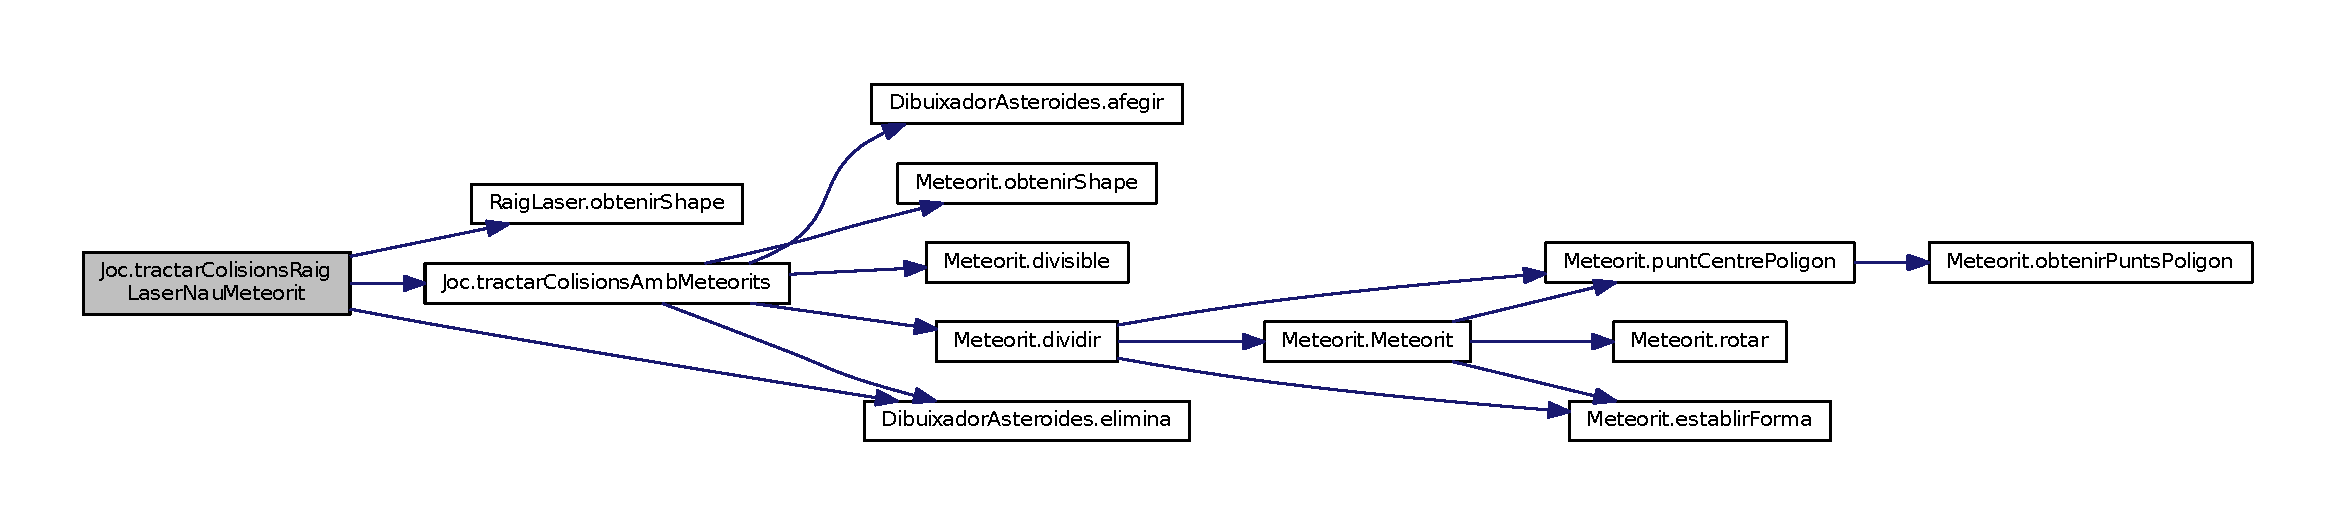
\includegraphics[width=350pt]{class_joc_a9a3116242cc69985726f4825be70a9b5_cgraph}
\end{center}
\end{figure}




Here is the caller graph for this function\+:\nopagebreak
\begin{figure}[H]
\begin{center}
\leavevmode
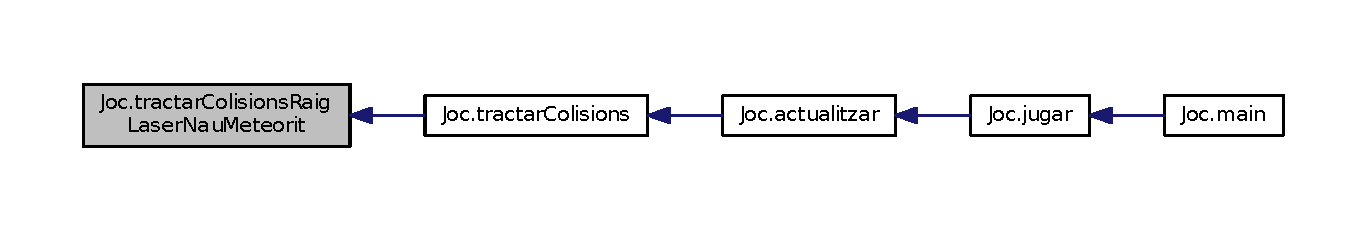
\includegraphics[width=350pt]{class_joc_a9a3116242cc69985726f4825be70a9b5_icgraph}
\end{center}
\end{figure}


\hypertarget{class_joc_af717aa44d1134343a67fc08374c3af45}{}\index{Joc@{Joc}!tractar\+Colisions\+Raig\+Laser\+N\+E\+Meteorit@{tractar\+Colisions\+Raig\+Laser\+N\+E\+Meteorit}}
\index{tractar\+Colisions\+Raig\+Laser\+N\+E\+Meteorit@{tractar\+Colisions\+Raig\+Laser\+N\+E\+Meteorit}!Joc@{Joc}}
\subsubsection[{tractar\+Colisions\+Raig\+Laser\+N\+E\+Meteorit}]{\setlength{\rightskip}{0pt plus 5cm}void Joc.\+tractar\+Colisions\+Raig\+Laser\+N\+E\+Meteorit (
\begin{DoxyParamCaption}
{}
\end{DoxyParamCaption}
) throws Exception\hspace{0.3cm}{\ttfamily [private]}}\label{class_joc_af717aa44d1134343a67fc08374c3af45}
\begin{DoxyPrecond}{Precondition}
-- 
\end{DoxyPrecond}
\begin{DoxyPostcond}{Postcondition}
els \hyperlink{class_raig_laser}{Raig\+Laser} que hagin col·lisionat amb un \hyperlink{class_meteorit}{Meteorit} s\textquotesingle{}han eliminat i els Meteorits 
\end{DoxyPostcond}


Definition at line 455 of file Joc.\+java.



Here is the call graph for this function\+:\nopagebreak
\begin{figure}[H]
\begin{center}
\leavevmode
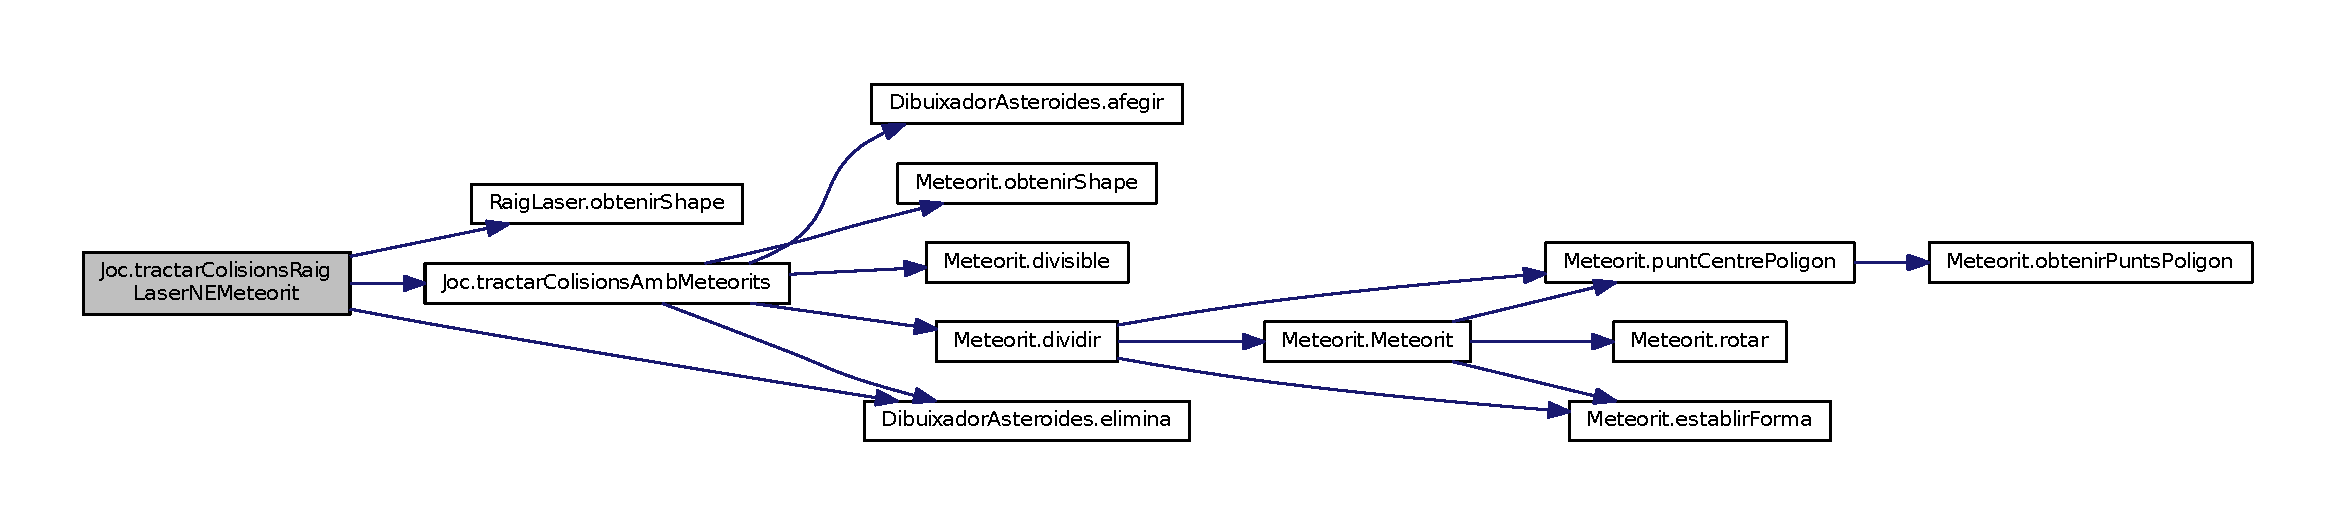
\includegraphics[width=350pt]{class_joc_af717aa44d1134343a67fc08374c3af45_cgraph}
\end{center}
\end{figure}




Here is the caller graph for this function\+:\nopagebreak
\begin{figure}[H]
\begin{center}
\leavevmode
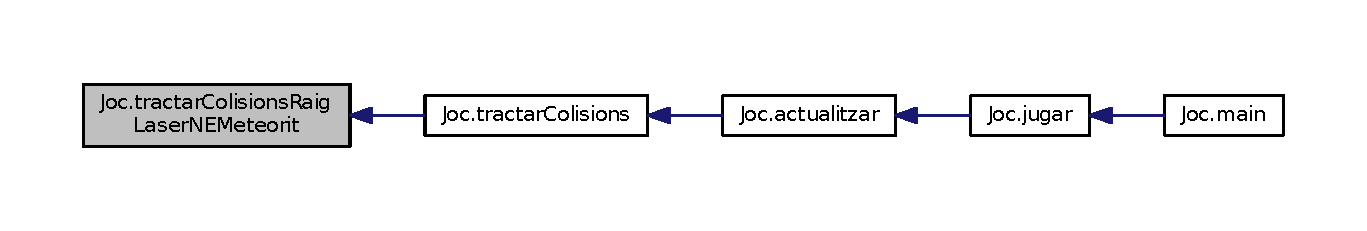
\includegraphics[width=350pt]{class_joc_af717aa44d1134343a67fc08374c3af45_icgraph}
\end{center}
\end{figure}


\hypertarget{class_joc_a84da80994a7dd370b3772cf962500617}{}\index{Joc@{Joc}!xocar\+Nau\+Enemiga@{xocar\+Nau\+Enemiga}}
\index{xocar\+Nau\+Enemiga@{xocar\+Nau\+Enemiga}!Joc@{Joc}}
\subsubsection[{xocar\+Nau\+Enemiga}]{\setlength{\rightskip}{0pt plus 5cm}void Joc.\+xocar\+Nau\+Enemiga (
\begin{DoxyParamCaption}
{}
\end{DoxyParamCaption}
) throws Exception\hspace{0.3cm}{\ttfamily [private]}}\label{class_joc_a84da80994a7dd370b3772cf962500617}
\begin{DoxyPrecond}{Precondition}
-- 
\end{DoxyPrecond}
\begin{DoxyPostcond}{Postcondition}
la \hyperlink{class_nau_enemiga}{Nau\+Enemiga} desapareix del \hyperlink{class_joc}{Joc} durant 5 segons, la puntuació incrementa 100 punts 
\end{DoxyPostcond}


Definition at line 414 of file Joc.\+java.



Here is the call graph for this function\+:\nopagebreak
\begin{figure}[H]
\begin{center}
\leavevmode
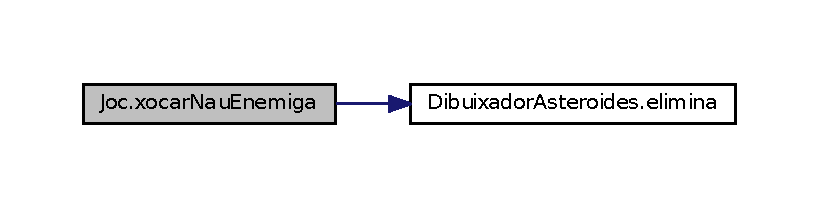
\includegraphics[width=350pt]{class_joc_a84da80994a7dd370b3772cf962500617_cgraph}
\end{center}
\end{figure}




Here is the caller graph for this function\+:\nopagebreak
\begin{figure}[H]
\begin{center}
\leavevmode
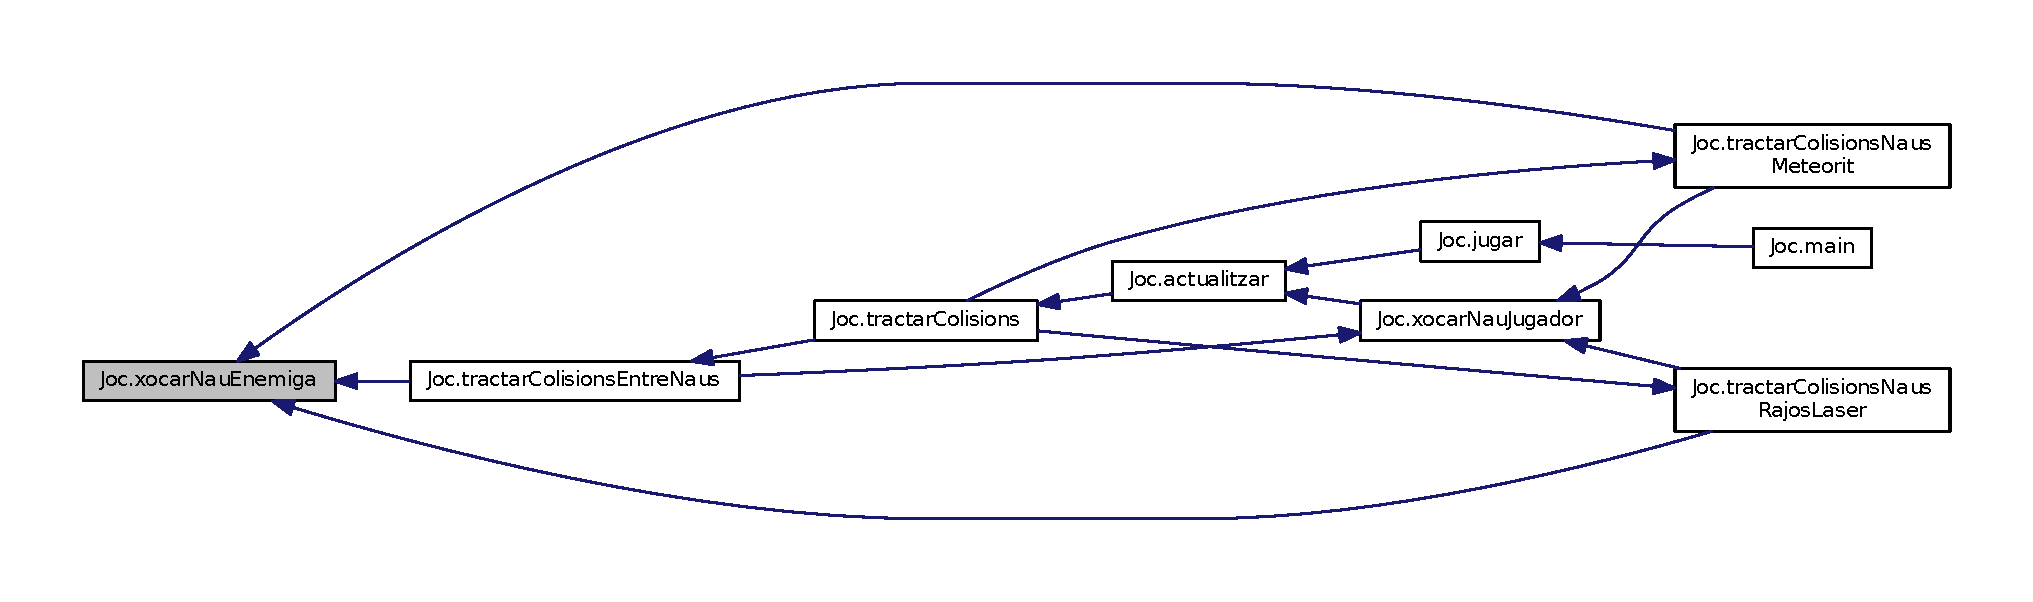
\includegraphics[width=350pt]{class_joc_a84da80994a7dd370b3772cf962500617_icgraph}
\end{center}
\end{figure}


\hypertarget{class_joc_a471c58ad94b7a8732a6b3e4695f2a691}{}\index{Joc@{Joc}!xocar\+Nau\+Jugador@{xocar\+Nau\+Jugador}}
\index{xocar\+Nau\+Jugador@{xocar\+Nau\+Jugador}!Joc@{Joc}}
\subsubsection[{xocar\+Nau\+Jugador}]{\setlength{\rightskip}{0pt plus 5cm}void Joc.\+xocar\+Nau\+Jugador (
\begin{DoxyParamCaption}
{}
\end{DoxyParamCaption}
) throws Exception\hspace{0.3cm}{\ttfamily [private]}}\label{class_joc_a471c58ad94b7a8732a6b3e4695f2a691}
\begin{DoxyPrecond}{Precondition}
-- 
\end{DoxyPrecond}
\begin{DoxyPostcond}{Postcondition}
si la nau està viva es centra la nau i se li resta una vida, altrament s\textquotesingle{}acaba la partida i es mostra un missatge. Si té 0 vides, mor. 
\end{DoxyPostcond}


Definition at line 384 of file Joc.\+java.



Here is the call graph for this function\+:\nopagebreak
\begin{figure}[H]
\begin{center}
\leavevmode
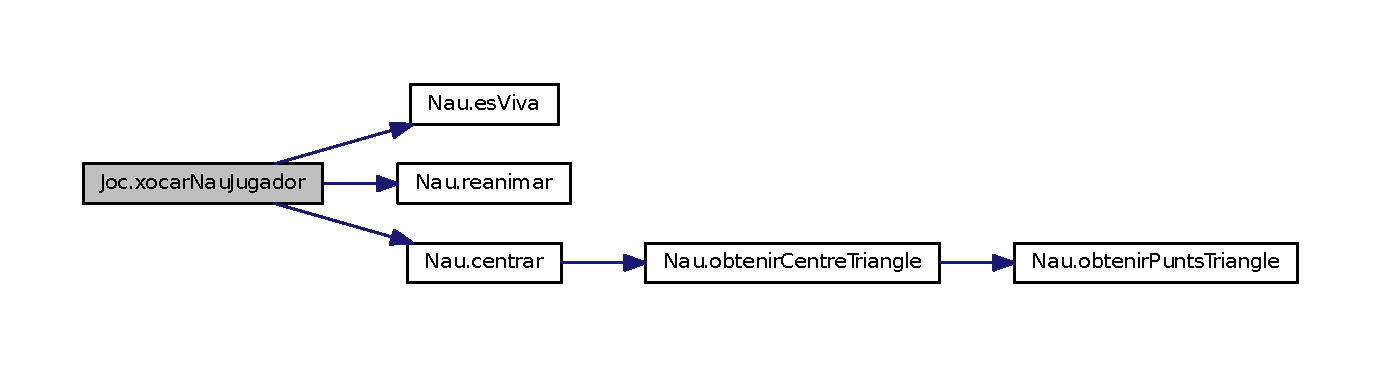
\includegraphics[width=350pt]{class_joc_a471c58ad94b7a8732a6b3e4695f2a691_cgraph}
\end{center}
\end{figure}




Here is the caller graph for this function\+:\nopagebreak
\begin{figure}[H]
\begin{center}
\leavevmode
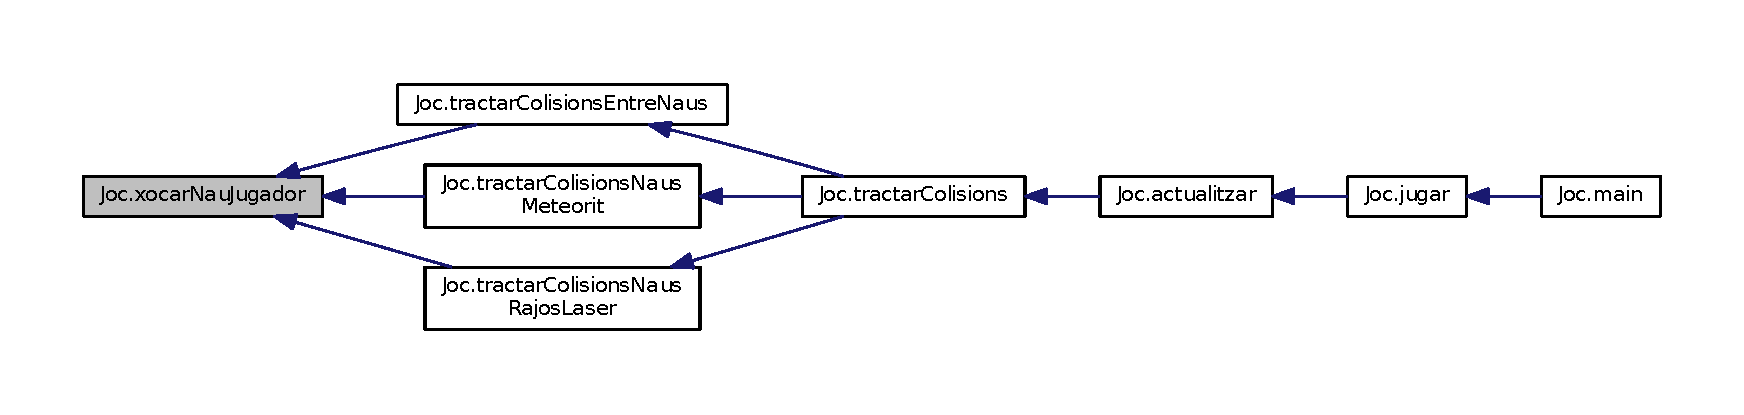
\includegraphics[width=350pt]{class_joc_a471c58ad94b7a8732a6b3e4695f2a691_icgraph}
\end{center}
\end{figure}




The documentation for this class was generated from the following file\+:\begin{DoxyCompactItemize}
\item 
/mnt/\+Dades/\+Documents/uni/\+Pro\+P/asteroides/src/\hyperlink{_joc_8java}{Joc.\+java}\end{DoxyCompactItemize}

\hypertarget{class_meteorit}{}\section{Meteorit Class Reference}
\label{class_meteorit}\index{Meteorit@{Meteorit}}


És un meteorit amb forma de polígon irregular que pot tenir quatre tipus de formes diferents. També pot tenir dues mides, gran o petit.  




Inheritance diagram for Meteorit\+:\nopagebreak
\begin{figure}[H]
\begin{center}
\leavevmode
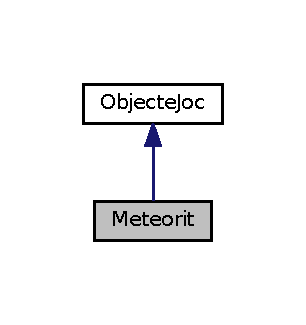
\includegraphics[width=147pt]{class_meteorit__inherit__graph}
\end{center}
\end{figure}


Collaboration diagram for Meteorit\+:\nopagebreak
\begin{figure}[H]
\begin{center}
\leavevmode
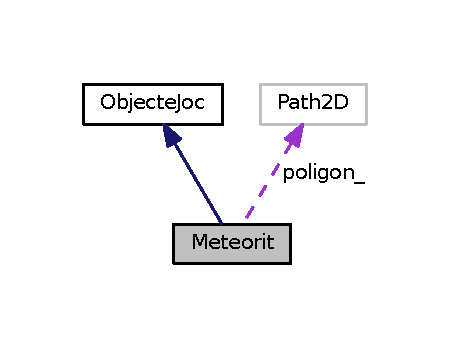
\includegraphics[width=216pt]{class_meteorit__coll__graph}
\end{center}
\end{figure}
\subsection*{Public Member Functions}
\begin{DoxyCompactItemize}
\item 
\hyperlink{class_meteorit_a9dcc96793a206baab2cc5aa5141a30f5}{Meteorit} (double velocitat, double angle, int mida, double x, double y)
\item 
void \hyperlink{class_meteorit_ab1e8e957f4ba216253d211523f2b3091}{situar\+Al\+Costat\+Mes\+Proper} (int amplada, int altura)
\item 
\hyperlink{class_meteorit}{Meteorit} \hyperlink{class_meteorit_aa4b891941b6ef30774a45d6965266170}{dividir} ()
\item 
boolean \hyperlink{class_meteorit_ab7f4539dc26a5026d8978918620db253}{divisible} ()
\item 
void \hyperlink{class_meteorit_af23ae6e1b16f750542711547cbe4957c}{moure} (int amplada, int altura)
\item 
double\mbox{[}$\,$\mbox{]} \hyperlink{class_meteorit_a685d6a89435a2fb03f1d8ebdeb70cb14}{punt\+Vertex\+Mes\+Proper} (double x, double y)
\item 
void \hyperlink{class_meteorit_a28f9530c5db8c8a192b272b8bd1114d2}{dibuixar} (Graphics2\+D g2)
\item 
Shape \hyperlink{class_meteorit_a31192464dbdc8e1bac9ae57c87ac6e2b}{obtenir\+Shape} ()
\end{DoxyCompactItemize}
\subsection*{Private Member Functions}
\begin{DoxyCompactItemize}
\item 
double\mbox{[}$\,$\mbox{]} \hyperlink{class_meteorit_a353fa1242e850f582f792605167e58e7}{punt\+Mes\+Allunyat} (double\mbox{[}$\,$\mbox{]} punt)
\item 
void \hyperlink{class_meteorit_a429daccf37f941ac0395a1838f0991a2}{rotar} (int graus)
\item 
void \hyperlink{class_meteorit_a0bc8468013d85caed1efe51b98397069}{establir\+Forma} (double x, double y, int forma)
\item 
boolean \hyperlink{class_meteorit_ac447d4590c8de8fd6153402a512adee2}{ha\+Sortit} (int amplada, int altura)
\item 
double\mbox{[}$\,$\mbox{]} \hyperlink{class_meteorit_ab63300b6281833f51f228bf8fb49c035}{punt\+Proper\+Al\+Centre\+De\+Area} (int amplada, int altura)
\item 
double\mbox{[}$\,$\mbox{]} \hyperlink{class_meteorit_aec4418bf83baf51641639ef97407b03f}{punt\+Llunya\+Al\+Centre\+De\+Area} (int amplada, int altura)
\item 
double\mbox{[}$\,$\mbox{]} \hyperlink{class_meteorit_a8d316ea738e82c4c9b2e02bc787e8bdc}{punt\+Centre\+Poligon} ()
\item 
double\mbox{[}$\,$\mbox{]} \hyperlink{class_meteorit_a237af5bb28238c5e76d1cea55b4457b6}{obtenir\+Punts\+Poligon} ()
\end{DoxyCompactItemize}
\subsection*{Private Attributes}
\begin{DoxyCompactItemize}
\item 
Path2\+D \hyperlink{class_meteorit_a1dd8a11e4ec8c806ee66a50773daeaf7}{poligon\+\_\+}
\begin{DoxyCompactList}\small\item\em Camí geomètric que forma un polígon irregular tancat (pot contenir quatre formes diferents) i dues mides. \end{DoxyCompactList}\item 
int \hyperlink{class_meteorit_a8edd607e17be6537c15ab04bfd29dc52}{mida\+\_\+}
\begin{DoxyCompactList}\small\item\em Val 1 si el \hyperlink{class_meteorit}{Meteorit} és gran i 2 si és petit. \end{DoxyCompactList}\item 
double \hyperlink{class_meteorit_a6d567bfb1f4d118c6c36c7bff76ec28a}{velocitat\+\_\+}
\begin{DoxyCompactList}\small\item\em Mòdul del vector velocitat del \hyperlink{class_meteorit}{Meteorit}. \end{DoxyCompactList}\item 
double \hyperlink{class_meteorit_ae642e495aeb2d78122cb2ae550dde61b}{angle\+Velocitat\+\_\+}
\begin{DoxyCompactList}\small\item\em Angle\+\_\+ del vector velocitat del \hyperlink{class_meteorit}{Meteorit}. \end{DoxyCompactList}\item 
int \hyperlink{class_meteorit_a3b015faa09e271a0e54de95d1c9716c6}{n\+Vertexs\+\_\+}
\begin{DoxyCompactList}\small\item\em Nombre de vèrtexs que té el \hyperlink{class_meteorit}{Meteorit}. \end{DoxyCompactList}\end{DoxyCompactItemize}


\subsection{Detailed Description}
És un meteorit amb forma de polígon irregular que pot tenir quatre tipus de formes diferents. També pot tenir dues mides, gran o petit. 

\subsubsection*{Comportament bàsic\+: }

Apareix en la posició donada al constructor, coordenada (x,y)
\begin{DoxyItemize}
\item Es mou en una direcció i velocitat fixes, la velocitat és donada al constructor, la direcció és aleatòria
\item És controlat per la màquina
\item Segons la mida (1 o 2) serà gran o petit, respectivament
\item Quan un \hyperlink{class_meteorit}{Meteorit} es crea, té mida 1 (gran) i es rota el polígon un angle aleatori
\item Si és un \hyperlink{class_meteorit}{Meteorit} gran, pot ser destruit en dos Meteorits de forma i direcció aleatòries, de mida petita
\item Si es destrueix un meteorit petit, desapareix
\end{DoxyItemize}

\subsubsection*{Supòsits sobre l\textquotesingle{}area(a) on es mou el \hyperlink{class_meteorit}{Meteorit}\+: }

Té mida fixa i no canvia mentre existeix el \hyperlink{class_meteorit}{Meteorit} És un pla amb\+:
\begin{DoxyItemize}
\item un eix horitzontal X que augmenta d\textquotesingle{}esquerra a dreta (dreta és més)
\end{DoxyItemize}

un eix vertical Y que augmenta de dalt a baix (a baix és més) 

Definition at line 30 of file Meteorit.\+java.



\subsection{Constructor \& Destructor Documentation}
\hypertarget{class_meteorit_a9dcc96793a206baab2cc5aa5141a30f5}{}\index{Meteorit@{Meteorit}!Meteorit@{Meteorit}}
\index{Meteorit@{Meteorit}!Meteorit@{Meteorit}}
\subsubsection[{Meteorit}]{\setlength{\rightskip}{0pt plus 5cm}Meteorit.\+Meteorit (
\begin{DoxyParamCaption}
\item[{double}]{velocitat, }
\item[{double}]{angle, }
\item[{int}]{mida, }
\item[{double}]{x, }
\item[{double}]{y}
\end{DoxyParamCaption}
)}\label{class_meteorit_a9dcc96793a206baab2cc5aa5141a30f5}
\begin{DoxyPrecond}{Precondition}
-- 
\end{DoxyPrecond}
\begin{DoxyPostcond}{Postcondition}
el \hyperlink{class_meteorit}{Meteorit} té una velocitat v, una direcció angle i una mida m, està situat a (x,y) 
\end{DoxyPostcond}


Definition at line 54 of file Meteorit.\+java.



Here is the call graph for this function\+:\nopagebreak
\begin{figure}[H]
\begin{center}
\leavevmode
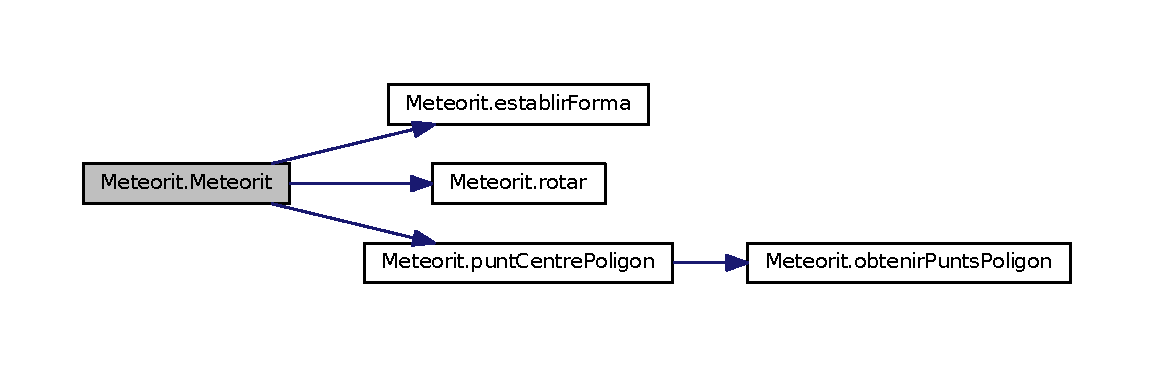
\includegraphics[width=350pt]{class_meteorit_a9dcc96793a206baab2cc5aa5141a30f5_cgraph}
\end{center}
\end{figure}




Here is the caller graph for this function\+:\nopagebreak
\begin{figure}[H]
\begin{center}
\leavevmode
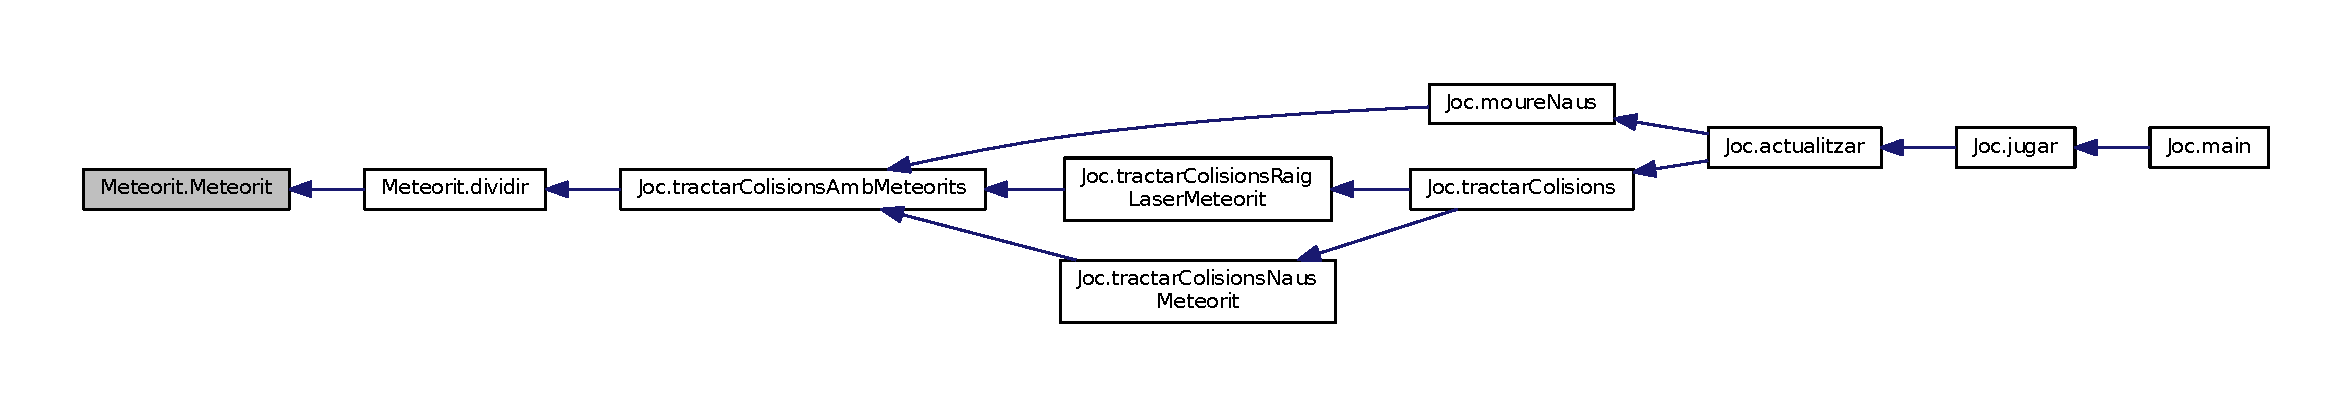
\includegraphics[width=350pt]{class_meteorit_a9dcc96793a206baab2cc5aa5141a30f5_icgraph}
\end{center}
\end{figure}




\subsection{Member Function Documentation}
\hypertarget{class_meteorit_a28f9530c5db8c8a192b272b8bd1114d2}{}\index{Meteorit@{Meteorit}!dibuixar@{dibuixar}}
\index{dibuixar@{dibuixar}!Meteorit@{Meteorit}}
\subsubsection[{dibuixar}]{\setlength{\rightskip}{0pt plus 5cm}void Meteorit.\+dibuixar (
\begin{DoxyParamCaption}
\item[{Graphics2\+D}]{g2}
\end{DoxyParamCaption}
)}\label{class_meteorit_a28f9530c5db8c8a192b272b8bd1114d2}
\begin{DoxyPrecond}{Precondition}
-- 
\end{DoxyPrecond}
\begin{DoxyPostcond}{Postcondition}
dibuixa el \hyperlink{class_meteorit}{Meteorit} de contorn blanc a g2 
\end{DoxyPostcond}


Implements \hyperlink{interface_objecte_joc_a0d472e898df5faf145a2480ab51e3ef8}{Objecte\+Joc}.



Definition at line 369 of file Meteorit.\+java.

\hypertarget{class_meteorit_aa4b891941b6ef30774a45d6965266170}{}\index{Meteorit@{Meteorit}!dividir@{dividir}}
\index{dividir@{dividir}!Meteorit@{Meteorit}}
\subsubsection[{dividir}]{\setlength{\rightskip}{0pt plus 5cm}{\bf Meteorit} Meteorit.\+dividir (
\begin{DoxyParamCaption}
{}
\end{DoxyParamCaption}
)}\label{class_meteorit_aa4b891941b6ef30774a45d6965266170}
\begin{DoxyPrecond}{Precondition}
el \hyperlink{class_meteorit}{Meteorit} és gran 
\end{DoxyPrecond}
\begin{DoxyPostcond}{Postcondition}
el \hyperlink{class_meteorit}{Meteorit} s\textquotesingle{}ha reduit a petit i es situa al centre del \hyperlink{class_meteorit}{Meteorit} inicial, es retorna un altre \hyperlink{class_meteorit}{Meteorit} també de mida petita amb forma i direcció aleatòries, situat també al centre del \hyperlink{class_meteorit}{Meteorit} inicial, l\textquotesingle{}angle de velocitat del \hyperlink{class_meteorit}{Meteorit} retornat és diferent en 45 graus com a mínim respecte l\textquotesingle{}angle de velocitat de m 
\end{DoxyPostcond}


Definition at line 187 of file Meteorit.\+java.



Here is the call graph for this function\+:\nopagebreak
\begin{figure}[H]
\begin{center}
\leavevmode
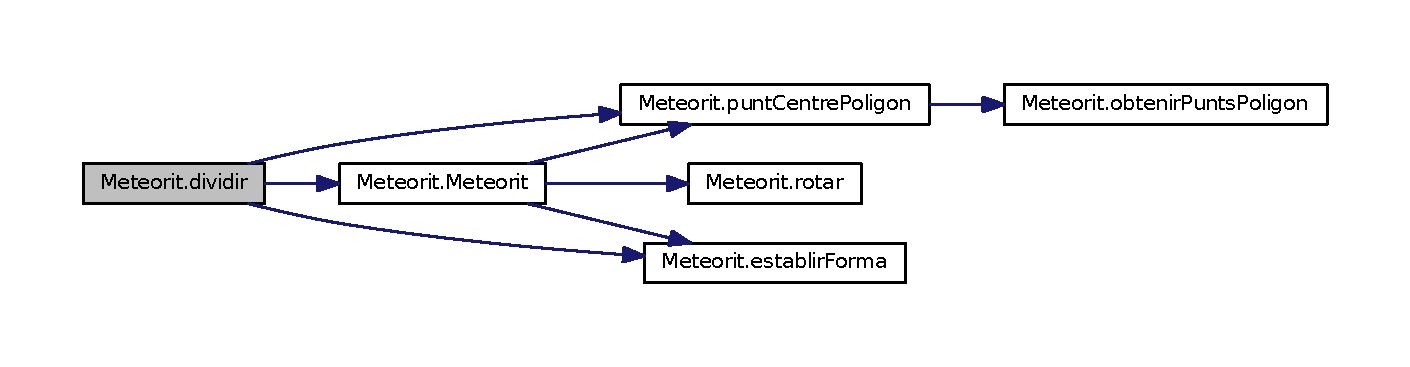
\includegraphics[width=350pt]{class_meteorit_aa4b891941b6ef30774a45d6965266170_cgraph}
\end{center}
\end{figure}




Here is the caller graph for this function\+:\nopagebreak
\begin{figure}[H]
\begin{center}
\leavevmode
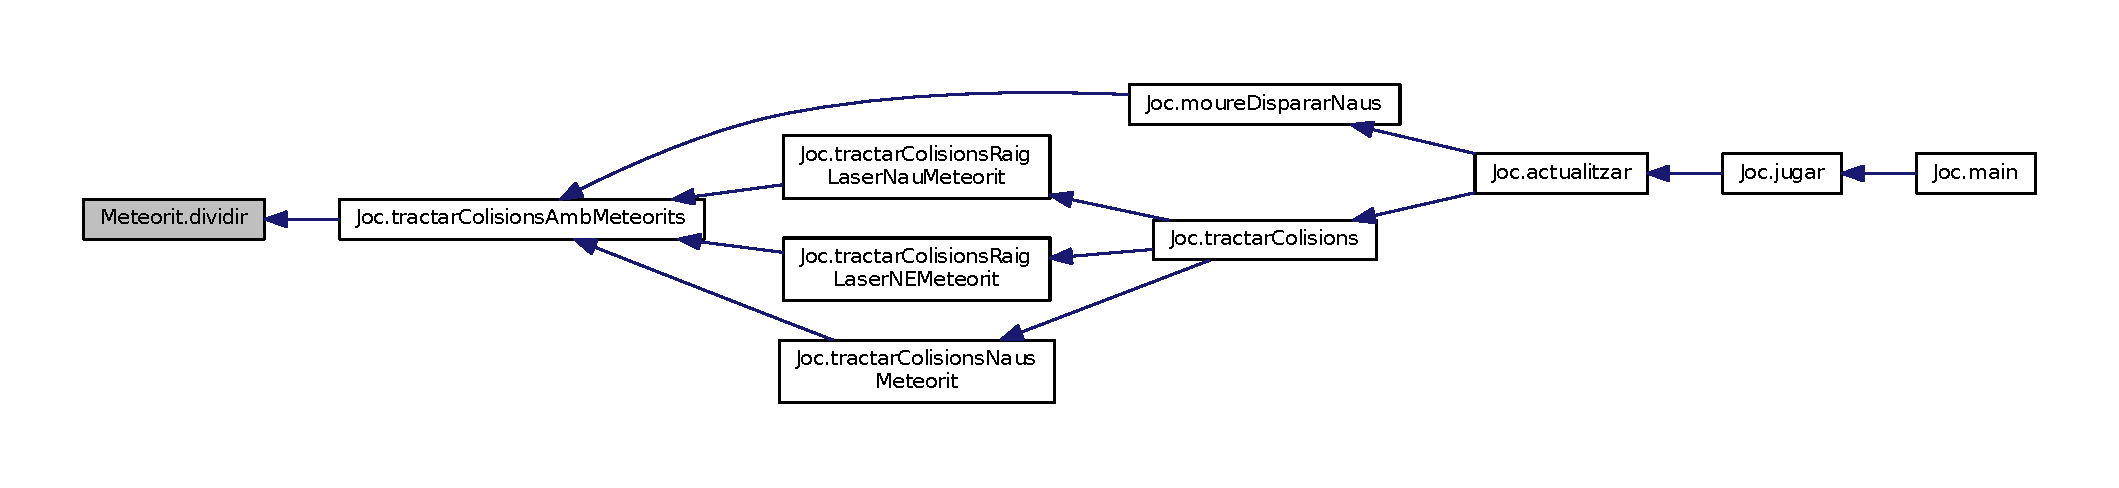
\includegraphics[width=350pt]{class_meteorit_aa4b891941b6ef30774a45d6965266170_icgraph}
\end{center}
\end{figure}


\hypertarget{class_meteorit_ab7f4539dc26a5026d8978918620db253}{}\index{Meteorit@{Meteorit}!divisible@{divisible}}
\index{divisible@{divisible}!Meteorit@{Meteorit}}
\subsubsection[{divisible}]{\setlength{\rightskip}{0pt plus 5cm}boolean Meteorit.\+divisible (
\begin{DoxyParamCaption}
{}
\end{DoxyParamCaption}
)}\label{class_meteorit_ab7f4539dc26a5026d8978918620db253}
\begin{DoxyPrecond}{Precondition}
-- 
\end{DoxyPrecond}
\begin{DoxyPostcond}{Postcondition}
retorna si el \hyperlink{class_meteorit}{Meteorit} és divisible 
\end{DoxyPostcond}


Definition at line 209 of file Meteorit.\+java.



Here is the caller graph for this function\+:\nopagebreak
\begin{figure}[H]
\begin{center}
\leavevmode
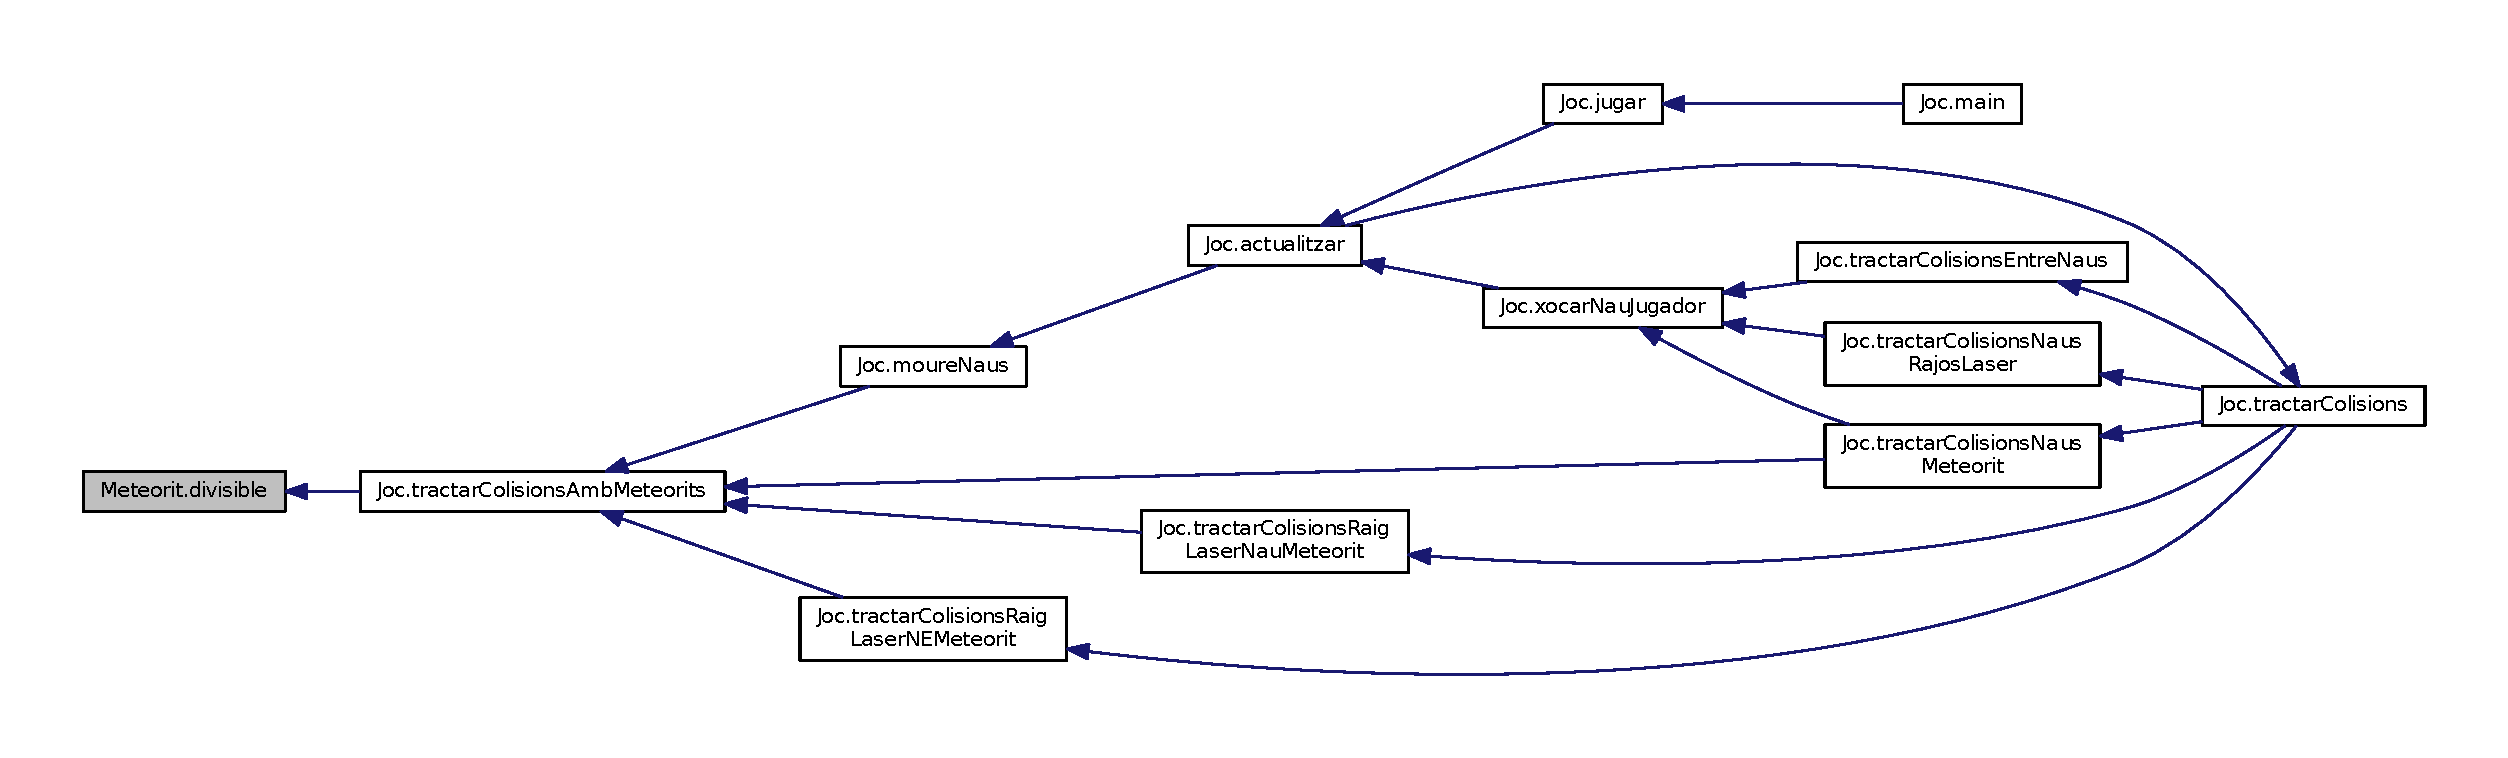
\includegraphics[width=350pt]{class_meteorit_ab7f4539dc26a5026d8978918620db253_icgraph}
\end{center}
\end{figure}


\hypertarget{class_meteorit_a0bc8468013d85caed1efe51b98397069}{}\index{Meteorit@{Meteorit}!establir\+Forma@{establir\+Forma}}
\index{establir\+Forma@{establir\+Forma}!Meteorit@{Meteorit}}
\subsubsection[{establir\+Forma}]{\setlength{\rightskip}{0pt plus 5cm}void Meteorit.\+establir\+Forma (
\begin{DoxyParamCaption}
\item[{double}]{x, }
\item[{double}]{y, }
\item[{int}]{forma}
\end{DoxyParamCaption}
)\hspace{0.3cm}{\ttfamily [private]}}\label{class_meteorit_a0bc8468013d85caed1efe51b98397069}
\begin{DoxyPrecond}{Precondition}
la mida és 1 o 2 
\end{DoxyPrecond}
\begin{DoxyPostcond}{Postcondition}
el \hyperlink{class_meteorit}{Meteorit} conté el dibuix 1, 2, 3 o 4 segons forma, aplicant-\/li la seva mida 
\end{DoxyPostcond}


Definition at line 132 of file Meteorit.\+java.



Here is the caller graph for this function\+:\nopagebreak
\begin{figure}[H]
\begin{center}
\leavevmode
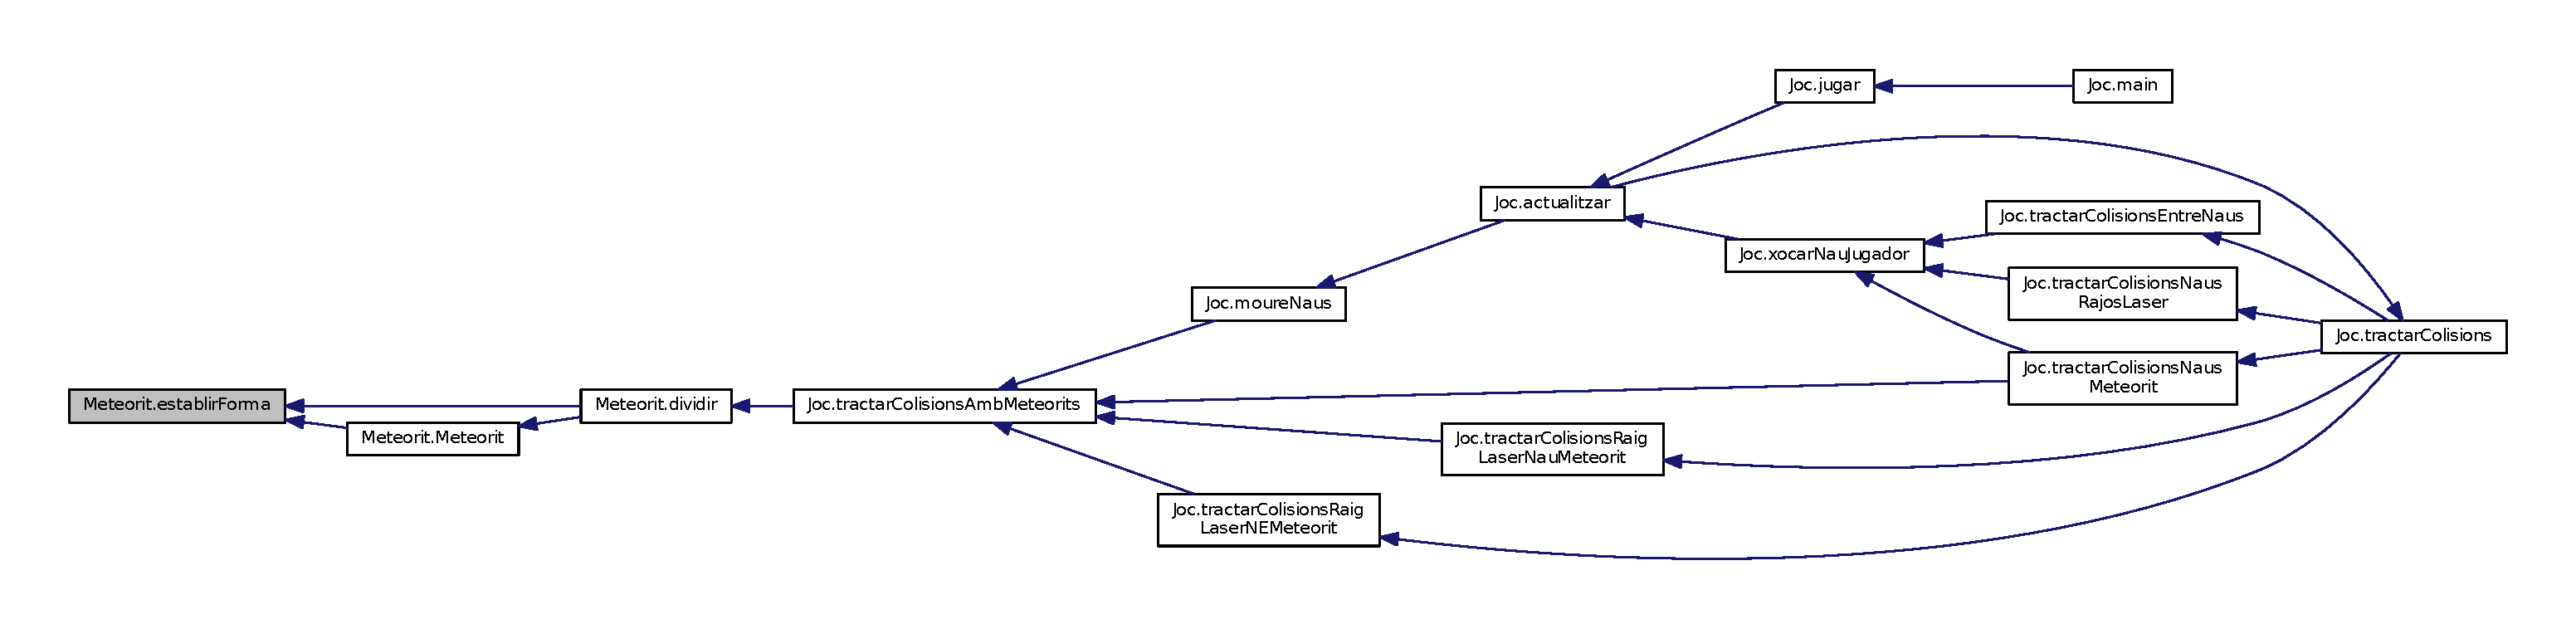
\includegraphics[width=350pt]{class_meteorit_a0bc8468013d85caed1efe51b98397069_icgraph}
\end{center}
\end{figure}


\hypertarget{class_meteorit_ac447d4590c8de8fd6153402a512adee2}{}\index{Meteorit@{Meteorit}!ha\+Sortit@{ha\+Sortit}}
\index{ha\+Sortit@{ha\+Sortit}!Meteorit@{Meteorit}}
\subsubsection[{ha\+Sortit}]{\setlength{\rightskip}{0pt plus 5cm}boolean Meteorit.\+ha\+Sortit (
\begin{DoxyParamCaption}
\item[{int}]{amplada, }
\item[{int}]{altura}
\end{DoxyParamCaption}
)\hspace{0.3cm}{\ttfamily [private]}}\label{class_meteorit_ac447d4590c8de8fd6153402a512adee2}
\begin{DoxyPrecond}{Precondition}
amplada $>$ 0 i altura $>$ 0 
\end{DoxyPrecond}
\begin{DoxyPostcond}{Postcondition}
diu si el \hyperlink{class_meteorit}{Meteorit} ha sortit de l\textquotesingle{}area amplada$\ast$altura 
\end{DoxyPostcond}


Definition at line 266 of file Meteorit.\+java.



Here is the call graph for this function\+:\nopagebreak
\begin{figure}[H]
\begin{center}
\leavevmode
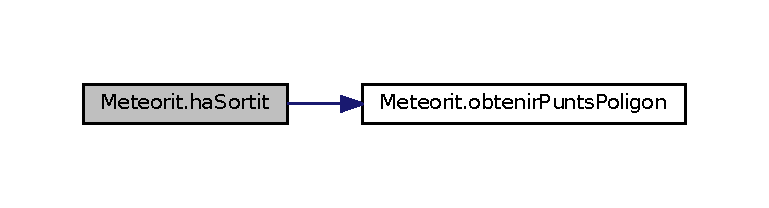
\includegraphics[width=350pt]{class_meteorit_ac447d4590c8de8fd6153402a512adee2_cgraph}
\end{center}
\end{figure}




Here is the caller graph for this function\+:\nopagebreak
\begin{figure}[H]
\begin{center}
\leavevmode
\includegraphics[width=305pt]{class_meteorit_ac447d4590c8de8fd6153402a512adee2_icgraph}
\end{center}
\end{figure}


\hypertarget{class_meteorit_af23ae6e1b16f750542711547cbe4957c}{}\index{Meteorit@{Meteorit}!moure@{moure}}
\index{moure@{moure}!Meteorit@{Meteorit}}
\subsubsection[{moure}]{\setlength{\rightskip}{0pt plus 5cm}void Meteorit.\+moure (
\begin{DoxyParamCaption}
\item[{int}]{amplada, }
\item[{int}]{altura}
\end{DoxyParamCaption}
)}\label{class_meteorit_af23ae6e1b16f750542711547cbe4957c}
\begin{DoxyPrecond}{Precondition}
amplada $>$ 0 i altura $>$ 0 
\end{DoxyPrecond}
\begin{DoxyPostcond}{Postcondition}
Desplaça el \hyperlink{class_meteorit}{Meteorit} a la posició(p) determinada per totes les velocitats del \hyperlink{class_meteorit}{Meteorit} Si el \hyperlink{class_meteorit}{Meteorit}, situat a la posició p, està totalment fora de l\textquotesingle{}area amplada$\ast$altura llavors el \hyperlink{class_meteorit}{Meteorit} es teletransporta al marge/costat invers del qual ha sortit(superior, inferior, esquerra, dreta) 
\end{DoxyPostcond}


Definition at line 217 of file Meteorit.\+java.



Here is the call graph for this function\+:\nopagebreak
\begin{figure}[H]
\begin{center}
\leavevmode
\includegraphics[width=350pt]{class_meteorit_af23ae6e1b16f750542711547cbe4957c_cgraph}
\end{center}
\end{figure}


\hypertarget{class_meteorit_a237af5bb28238c5e76d1cea55b4457b6}{}\index{Meteorit@{Meteorit}!obtenir\+Punts\+Poligon@{obtenir\+Punts\+Poligon}}
\index{obtenir\+Punts\+Poligon@{obtenir\+Punts\+Poligon}!Meteorit@{Meteorit}}
\subsubsection[{obtenir\+Punts\+Poligon}]{\setlength{\rightskip}{0pt plus 5cm}double \mbox{[}$\,$\mbox{]} Meteorit.\+obtenir\+Punts\+Poligon (
\begin{DoxyParamCaption}
{}
\end{DoxyParamCaption}
)\hspace{0.3cm}{\ttfamily [private]}}\label{class_meteorit_a237af5bb28238c5e76d1cea55b4457b6}
\begin{DoxyPrecond}{Precondition}
-- 
\end{DoxyPrecond}
\begin{DoxyPostcond}{Postcondition}
retorna una taula(t) que conte els punts del poligon coordenada (t\mbox{[}i\mbox{]},t\mbox{[}i+1\mbox{]}) per i = 0 fins al nombre de vèrtexs$\ast$2-\/2 increment 2 
\end{DoxyPostcond}


Definition at line 351 of file Meteorit.\+java.



Here is the caller graph for this function\+:\nopagebreak
\begin{figure}[H]
\begin{center}
\leavevmode
\includegraphics[width=350pt]{class_meteorit_a237af5bb28238c5e76d1cea55b4457b6_icgraph}
\end{center}
\end{figure}


\hypertarget{class_meteorit_a31192464dbdc8e1bac9ae57c87ac6e2b}{}\index{Meteorit@{Meteorit}!obtenir\+Shape@{obtenir\+Shape}}
\index{obtenir\+Shape@{obtenir\+Shape}!Meteorit@{Meteorit}}
\subsubsection[{obtenir\+Shape}]{\setlength{\rightskip}{0pt plus 5cm}Shape Meteorit.\+obtenir\+Shape (
\begin{DoxyParamCaption}
{}
\end{DoxyParamCaption}
)}\label{class_meteorit_a31192464dbdc8e1bac9ae57c87ac6e2b}
\begin{DoxyPrecond}{Precondition}
-- 
\end{DoxyPrecond}
\begin{DoxyPostcond}{Postcondition}
retorna el polígon del \hyperlink{class_meteorit}{Meteorit} 
\end{DoxyPostcond}


Definition at line 376 of file Meteorit.\+java.



Here is the caller graph for this function\+:\nopagebreak
\begin{figure}[H]
\begin{center}
\leavevmode
\includegraphics[width=350pt]{class_meteorit_a31192464dbdc8e1bac9ae57c87ac6e2b_icgraph}
\end{center}
\end{figure}


\hypertarget{class_meteorit_a8d316ea738e82c4c9b2e02bc787e8bdc}{}\index{Meteorit@{Meteorit}!punt\+Centre\+Poligon@{punt\+Centre\+Poligon}}
\index{punt\+Centre\+Poligon@{punt\+Centre\+Poligon}!Meteorit@{Meteorit}}
\subsubsection[{punt\+Centre\+Poligon}]{\setlength{\rightskip}{0pt plus 5cm}double \mbox{[}$\,$\mbox{]} Meteorit.\+punt\+Centre\+Poligon (
\begin{DoxyParamCaption}
{}
\end{DoxyParamCaption}
)\hspace{0.3cm}{\ttfamily [private]}}\label{class_meteorit_a8d316ea738e82c4c9b2e02bc787e8bdc}
\begin{DoxyPrecond}{Precondition}
-- 
\end{DoxyPrecond}
\begin{DoxyPostcond}{Postcondition}
retorna una taula t on t\mbox{[}0\mbox{]} i t\mbox{[}1\mbox{]} són les coordenades x i y del centre del polígon 
\end{DoxyPostcond}


Definition at line 315 of file Meteorit.\+java.



Here is the call graph for this function\+:\nopagebreak
\begin{figure}[H]
\begin{center}
\leavevmode
\includegraphics[width=350pt]{class_meteorit_a8d316ea738e82c4c9b2e02bc787e8bdc_cgraph}
\end{center}
\end{figure}




Here is the caller graph for this function\+:\nopagebreak
\begin{figure}[H]
\begin{center}
\leavevmode
\includegraphics[width=350pt]{class_meteorit_a8d316ea738e82c4c9b2e02bc787e8bdc_icgraph}
\end{center}
\end{figure}


\hypertarget{class_meteorit_aec4418bf83baf51641639ef97407b03f}{}\index{Meteorit@{Meteorit}!punt\+Llunya\+Al\+Centre\+De\+Area@{punt\+Llunya\+Al\+Centre\+De\+Area}}
\index{punt\+Llunya\+Al\+Centre\+De\+Area@{punt\+Llunya\+Al\+Centre\+De\+Area}!Meteorit@{Meteorit}}
\subsubsection[{punt\+Llunya\+Al\+Centre\+De\+Area}]{\setlength{\rightskip}{0pt plus 5cm}double \mbox{[}$\,$\mbox{]} Meteorit.\+punt\+Llunya\+Al\+Centre\+De\+Area (
\begin{DoxyParamCaption}
\item[{int}]{amplada, }
\item[{int}]{altura}
\end{DoxyParamCaption}
)\hspace{0.3cm}{\ttfamily [private]}}\label{class_meteorit_aec4418bf83baf51641639ef97407b03f}
\begin{DoxyPrecond}{Precondition}
amplada $>$ 0 i altura $>$ 0 
\end{DoxyPrecond}
\begin{DoxyPostcond}{Postcondition}
retorna una taula t on t\mbox{[}0\mbox{]} i t\mbox{[}1\mbox{]} són les coordenades x i y del punt del poligon més llunya al centre de l\textquotesingle{}area amplada$\ast$altura 
\end{DoxyPostcond}


Definition at line 297 of file Meteorit.\+java.



Here is the call graph for this function\+:\nopagebreak
\begin{figure}[H]
\begin{center}
\leavevmode
\includegraphics[width=350pt]{class_meteorit_aec4418bf83baf51641639ef97407b03f_cgraph}
\end{center}
\end{figure}




Here is the caller graph for this function\+:\nopagebreak
\begin{figure}[H]
\begin{center}
\leavevmode
\includegraphics[width=350pt]{class_meteorit_aec4418bf83baf51641639ef97407b03f_icgraph}
\end{center}
\end{figure}


\hypertarget{class_meteorit_a353fa1242e850f582f792605167e58e7}{}\index{Meteorit@{Meteorit}!punt\+Mes\+Allunyat@{punt\+Mes\+Allunyat}}
\index{punt\+Mes\+Allunyat@{punt\+Mes\+Allunyat}!Meteorit@{Meteorit}}
\subsubsection[{punt\+Mes\+Allunyat}]{\setlength{\rightskip}{0pt plus 5cm}double \mbox{[}$\,$\mbox{]} Meteorit.\+punt\+Mes\+Allunyat (
\begin{DoxyParamCaption}
\item[{double\mbox{[}$\,$\mbox{]}}]{punt}
\end{DoxyParamCaption}
)\hspace{0.3cm}{\ttfamily [private]}}\label{class_meteorit_a353fa1242e850f582f792605167e58e7}
\begin{DoxyPrecond}{Precondition}
-- 
\end{DoxyPrecond}
\begin{DoxyPostcond}{Postcondition}
retorna el punt més allunyat del \hyperlink{class_meteorit}{Meteorit} respecte punt 
\end{DoxyPostcond}


Definition at line 106 of file Meteorit.\+java.



Here is the call graph for this function\+:\nopagebreak
\begin{figure}[H]
\begin{center}
\leavevmode
\includegraphics[width=350pt]{class_meteorit_a353fa1242e850f582f792605167e58e7_cgraph}
\end{center}
\end{figure}




Here is the caller graph for this function\+:\nopagebreak
\begin{figure}[H]
\begin{center}
\leavevmode
\includegraphics[width=350pt]{class_meteorit_a353fa1242e850f582f792605167e58e7_icgraph}
\end{center}
\end{figure}


\hypertarget{class_meteorit_ab63300b6281833f51f228bf8fb49c035}{}\index{Meteorit@{Meteorit}!punt\+Proper\+Al\+Centre\+De\+Area@{punt\+Proper\+Al\+Centre\+De\+Area}}
\index{punt\+Proper\+Al\+Centre\+De\+Area@{punt\+Proper\+Al\+Centre\+De\+Area}!Meteorit@{Meteorit}}
\subsubsection[{punt\+Proper\+Al\+Centre\+De\+Area}]{\setlength{\rightskip}{0pt plus 5cm}double \mbox{[}$\,$\mbox{]} Meteorit.\+punt\+Proper\+Al\+Centre\+De\+Area (
\begin{DoxyParamCaption}
\item[{int}]{amplada, }
\item[{int}]{altura}
\end{DoxyParamCaption}
)\hspace{0.3cm}{\ttfamily [private]}}\label{class_meteorit_ab63300b6281833f51f228bf8fb49c035}
\begin{DoxyPrecond}{Precondition}
amplada $>$ 0 i altura $>$ 0 
\end{DoxyPrecond}
\begin{DoxyPostcond}{Postcondition}
retorna una taula t on t\mbox{[}0\mbox{]} i t\mbox{[}1\mbox{]} són les coordenades x i y del punt del poligon més proper al centre de l\textquotesingle{}area amplada$\ast$altura 
\end{DoxyPostcond}


Definition at line 279 of file Meteorit.\+java.



Here is the call graph for this function\+:\nopagebreak
\begin{figure}[H]
\begin{center}
\leavevmode
\includegraphics[width=350pt]{class_meteorit_ab63300b6281833f51f228bf8fb49c035_cgraph}
\end{center}
\end{figure}




Here is the caller graph for this function\+:\nopagebreak
\begin{figure}[H]
\begin{center}
\leavevmode
\includegraphics[width=350pt]{class_meteorit_ab63300b6281833f51f228bf8fb49c035_icgraph}
\end{center}
\end{figure}


\hypertarget{class_meteorit_a685d6a89435a2fb03f1d8ebdeb70cb14}{}\index{Meteorit@{Meteorit}!punt\+Vertex\+Mes\+Proper@{punt\+Vertex\+Mes\+Proper}}
\index{punt\+Vertex\+Mes\+Proper@{punt\+Vertex\+Mes\+Proper}!Meteorit@{Meteorit}}
\subsubsection[{punt\+Vertex\+Mes\+Proper}]{\setlength{\rightskip}{0pt plus 5cm}double \mbox{[}$\,$\mbox{]} Meteorit.\+punt\+Vertex\+Mes\+Proper (
\begin{DoxyParamCaption}
\item[{double}]{x, }
\item[{double}]{y}
\end{DoxyParamCaption}
)}\label{class_meteorit_a685d6a89435a2fb03f1d8ebdeb70cb14}
\begin{DoxyPrecond}{Precondition}
-- 
\end{DoxyPrecond}
\begin{DoxyPostcond}{Postcondition}
retorna la distància entre el punt (x,y) i el punt més proper del \hyperlink{class_meteorit}{Meteorit} 
\end{DoxyPostcond}


Definition at line 332 of file Meteorit.\+java.



Here is the call graph for this function\+:\nopagebreak
\begin{figure}[H]
\begin{center}
\leavevmode
\includegraphics[width=350pt]{class_meteorit_a685d6a89435a2fb03f1d8ebdeb70cb14_cgraph}
\end{center}
\end{figure}


\hypertarget{class_meteorit_a429daccf37f941ac0395a1838f0991a2}{}\index{Meteorit@{Meteorit}!rotar@{rotar}}
\index{rotar@{rotar}!Meteorit@{Meteorit}}
\subsubsection[{rotar}]{\setlength{\rightskip}{0pt plus 5cm}void Meteorit.\+rotar (
\begin{DoxyParamCaption}
\item[{int}]{graus}
\end{DoxyParamCaption}
)\hspace{0.3cm}{\ttfamily [private]}}\label{class_meteorit_a429daccf37f941ac0395a1838f0991a2}
\begin{DoxyPrecond}{Precondition}
-- 
\end{DoxyPrecond}
\begin{DoxyPostcond}{Postcondition}
rota el \hyperlink{class_meteorit}{Meteorit} un angle graus 
\end{DoxyPostcond}


Definition at line 124 of file Meteorit.\+java.



Here is the caller graph for this function\+:\nopagebreak
\begin{figure}[H]
\begin{center}
\leavevmode
\includegraphics[width=350pt]{class_meteorit_a429daccf37f941ac0395a1838f0991a2_icgraph}
\end{center}
\end{figure}


\hypertarget{class_meteorit_ab1e8e957f4ba216253d211523f2b3091}{}\index{Meteorit@{Meteorit}!situar\+Al\+Costat\+Mes\+Proper@{situar\+Al\+Costat\+Mes\+Proper}}
\index{situar\+Al\+Costat\+Mes\+Proper@{situar\+Al\+Costat\+Mes\+Proper}!Meteorit@{Meteorit}}
\subsubsection[{situar\+Al\+Costat\+Mes\+Proper}]{\setlength{\rightskip}{0pt plus 5cm}void Meteorit.\+situar\+Al\+Costat\+Mes\+Proper (
\begin{DoxyParamCaption}
\item[{int}]{amplada, }
\item[{int}]{altura}
\end{DoxyParamCaption}
)}\label{class_meteorit_ab1e8e957f4ba216253d211523f2b3091}
\begin{DoxyPrecond}{Precondition}
-- 
\end{DoxyPrecond}
\begin{DoxyPostcond}{Postcondition}
situa el \hyperlink{class_meteorit}{Meteorit} a la banda de la pantalla més propera d\textquotesingle{}on es troba el \hyperlink{class_meteorit}{Meteorit}. L\textquotesingle{}àrea de la pantalla és amplada$\ast$altura 
\end{DoxyPostcond}


Definition at line 73 of file Meteorit.\+java.



Here is the call graph for this function\+:\nopagebreak
\begin{figure}[H]
\begin{center}
\leavevmode
\includegraphics[width=350pt]{class_meteorit_ab1e8e957f4ba216253d211523f2b3091_cgraph}
\end{center}
\end{figure}




Here is the caller graph for this function\+:\nopagebreak
\begin{figure}[H]
\begin{center}
\leavevmode
\includegraphics[width=350pt]{class_meteorit_ab1e8e957f4ba216253d211523f2b3091_icgraph}
\end{center}
\end{figure}




\subsection{Member Data Documentation}
\hypertarget{class_meteorit_ae642e495aeb2d78122cb2ae550dde61b}{}\index{Meteorit@{Meteorit}!angle\+Velocitat\+\_\+@{angle\+Velocitat\+\_\+}}
\index{angle\+Velocitat\+\_\+@{angle\+Velocitat\+\_\+}!Meteorit@{Meteorit}}
\subsubsection[{angle\+Velocitat\+\_\+}]{\setlength{\rightskip}{0pt plus 5cm}double Meteorit.\+angle\+Velocitat\+\_\+\hspace{0.3cm}{\ttfamily [private]}}\label{class_meteorit_ae642e495aeb2d78122cb2ae550dde61b}


Angle\+\_\+ del vector velocitat del \hyperlink{class_meteorit}{Meteorit}. 



Definition at line 49 of file Meteorit.\+java.

\hypertarget{class_meteorit_a8edd607e17be6537c15ab04bfd29dc52}{}\index{Meteorit@{Meteorit}!mida\+\_\+@{mida\+\_\+}}
\index{mida\+\_\+@{mida\+\_\+}!Meteorit@{Meteorit}}
\subsubsection[{mida\+\_\+}]{\setlength{\rightskip}{0pt plus 5cm}int Meteorit.\+mida\+\_\+\hspace{0.3cm}{\ttfamily [private]}}\label{class_meteorit_a8edd607e17be6537c15ab04bfd29dc52}


Val 1 si el \hyperlink{class_meteorit}{Meteorit} és gran i 2 si és petit. 



Definition at line 47 of file Meteorit.\+java.

\hypertarget{class_meteorit_a3b015faa09e271a0e54de95d1c9716c6}{}\index{Meteorit@{Meteorit}!n\+Vertexs\+\_\+@{n\+Vertexs\+\_\+}}
\index{n\+Vertexs\+\_\+@{n\+Vertexs\+\_\+}!Meteorit@{Meteorit}}
\subsubsection[{n\+Vertexs\+\_\+}]{\setlength{\rightskip}{0pt plus 5cm}int Meteorit.\+n\+Vertexs\+\_\+\hspace{0.3cm}{\ttfamily [private]}}\label{class_meteorit_a3b015faa09e271a0e54de95d1c9716c6}


Nombre de vèrtexs que té el \hyperlink{class_meteorit}{Meteorit}. 



Definition at line 50 of file Meteorit.\+java.

\hypertarget{class_meteorit_a1dd8a11e4ec8c806ee66a50773daeaf7}{}\index{Meteorit@{Meteorit}!poligon\+\_\+@{poligon\+\_\+}}
\index{poligon\+\_\+@{poligon\+\_\+}!Meteorit@{Meteorit}}
\subsubsection[{poligon\+\_\+}]{\setlength{\rightskip}{0pt plus 5cm}Path2\+D Meteorit.\+poligon\+\_\+\hspace{0.3cm}{\ttfamily [private]}}\label{class_meteorit_a1dd8a11e4ec8c806ee66a50773daeaf7}


Camí geomètric que forma un polígon irregular tancat (pot contenir quatre formes diferents) i dues mides. 



Definition at line 46 of file Meteorit.\+java.

\hypertarget{class_meteorit_a6d567bfb1f4d118c6c36c7bff76ec28a}{}\index{Meteorit@{Meteorit}!velocitat\+\_\+@{velocitat\+\_\+}}
\index{velocitat\+\_\+@{velocitat\+\_\+}!Meteorit@{Meteorit}}
\subsubsection[{velocitat\+\_\+}]{\setlength{\rightskip}{0pt plus 5cm}double Meteorit.\+velocitat\+\_\+\hspace{0.3cm}{\ttfamily [private]}}\label{class_meteorit_a6d567bfb1f4d118c6c36c7bff76ec28a}


Mòdul del vector velocitat del \hyperlink{class_meteorit}{Meteorit}. 



Definition at line 48 of file Meteorit.\+java.



The documentation for this class was generated from the following file\+:\begin{DoxyCompactItemize}
\item 
/mnt/\+Dades/\+Documents/uni/\+Pro\+P/asteroides/src/\hyperlink{_meteorit_8java}{Meteorit.\+java}\end{DoxyCompactItemize}

\hypertarget{class_joc_1_1_my_key_listener}{}\section{Joc.\+My\+Key\+Listener Class Reference}
\label{class_joc_1_1_my_key_listener}\index{Joc.\+My\+Key\+Listener@{Joc.\+My\+Key\+Listener}}


Key\+Listener per a actualitzar els booleans segons les pulsacions del teclat.  




Inheritance diagram for Joc.\+My\+Key\+Listener\+:\nopagebreak
\begin{figure}[H]
\begin{center}
\leavevmode
\includegraphics[width=181pt]{class_joc_1_1_my_key_listener__inherit__graph}
\end{center}
\end{figure}


Collaboration diagram for Joc.\+My\+Key\+Listener\+:\nopagebreak
\begin{figure}[H]
\begin{center}
\leavevmode
\includegraphics[width=181pt]{class_joc_1_1_my_key_listener__coll__graph}
\end{center}
\end{figure}
\subsection*{Public Member Functions}
\begin{DoxyCompactItemize}
\item 
void \hyperlink{class_joc_1_1_my_key_listener_a4ca06e4f3950c3745be88c484f12df85}{key\+Typed} (Key\+Event e)
\item 
void \hyperlink{class_joc_1_1_my_key_listener_a14addef50fc960bcd8e4ce5cc3d9c643}{key\+Pressed} (Key\+Event e)
\item 
void \hyperlink{class_joc_1_1_my_key_listener_af5f550e0c17018b1bce4648782aaa9fb}{key\+Released} (Key\+Event e)
\end{DoxyCompactItemize}


\subsection{Detailed Description}
Key\+Listener per a actualitzar els booleans segons les pulsacions del teclat. 

Definition at line 576 of file Joc.\+java.



\subsection{Member Function Documentation}
\hypertarget{class_joc_1_1_my_key_listener_a14addef50fc960bcd8e4ce5cc3d9c643}{}\index{Joc\+::\+My\+Key\+Listener@{Joc\+::\+My\+Key\+Listener}!key\+Pressed@{key\+Pressed}}
\index{key\+Pressed@{key\+Pressed}!Joc\+::\+My\+Key\+Listener@{Joc\+::\+My\+Key\+Listener}}
\subsubsection[{key\+Pressed}]{\setlength{\rightskip}{0pt plus 5cm}void Joc.\+My\+Key\+Listener.\+key\+Pressed (
\begin{DoxyParamCaption}
\item[{Key\+Event}]{e}
\end{DoxyParamCaption}
)}\label{class_joc_1_1_my_key_listener_a14addef50fc960bcd8e4ce5cc3d9c643}


Definition at line 580 of file Joc.\+java.

\hypertarget{class_joc_1_1_my_key_listener_af5f550e0c17018b1bce4648782aaa9fb}{}\index{Joc\+::\+My\+Key\+Listener@{Joc\+::\+My\+Key\+Listener}!key\+Released@{key\+Released}}
\index{key\+Released@{key\+Released}!Joc\+::\+My\+Key\+Listener@{Joc\+::\+My\+Key\+Listener}}
\subsubsection[{key\+Released}]{\setlength{\rightskip}{0pt plus 5cm}void Joc.\+My\+Key\+Listener.\+key\+Released (
\begin{DoxyParamCaption}
\item[{Key\+Event}]{e}
\end{DoxyParamCaption}
)}\label{class_joc_1_1_my_key_listener_af5f550e0c17018b1bce4648782aaa9fb}


Definition at line 597 of file Joc.\+java.

\hypertarget{class_joc_1_1_my_key_listener_a4ca06e4f3950c3745be88c484f12df85}{}\index{Joc\+::\+My\+Key\+Listener@{Joc\+::\+My\+Key\+Listener}!key\+Typed@{key\+Typed}}
\index{key\+Typed@{key\+Typed}!Joc\+::\+My\+Key\+Listener@{Joc\+::\+My\+Key\+Listener}}
\subsubsection[{key\+Typed}]{\setlength{\rightskip}{0pt plus 5cm}void Joc.\+My\+Key\+Listener.\+key\+Typed (
\begin{DoxyParamCaption}
\item[{Key\+Event}]{e}
\end{DoxyParamCaption}
)}\label{class_joc_1_1_my_key_listener_a4ca06e4f3950c3745be88c484f12df85}


Definition at line 578 of file Joc.\+java.



The documentation for this class was generated from the following file\+:\begin{DoxyCompactItemize}
\item 
/mnt/\+Dades/\+Documents/uni/\+Pro\+P/asteroides/src/\hyperlink{_joc_8java}{Joc.\+java}\end{DoxyCompactItemize}

\hypertarget{class_nau}{}\section{Nau Class Reference}
\label{class_nau}\index{Nau@{Nau}}


És una nau espacial triangular isòsceles que es mou dins d\textquotesingle{}un espai definit.  




Inheritance diagram for Nau\+:\nopagebreak
\begin{figure}[H]
\begin{center}
\leavevmode
\includegraphics[width=158pt]{class_nau__inherit__graph}
\end{center}
\end{figure}


Collaboration diagram for Nau\+:\nopagebreak
\begin{figure}[H]
\begin{center}
\leavevmode
\includegraphics[width=275pt]{class_nau__coll__graph}
\end{center}
\end{figure}
\subsection*{Public Member Functions}
\begin{DoxyCompactItemize}
\item 
void \hyperlink{class_nau_a973eef3d7c7996553002b538481eadd6}{centrar} (int amplada, int altura)
\item 
\hyperlink{class_raig_laser}{Raig\+Laser} \hyperlink{class_nau_a7449b7bf128a70e305bc85781ee833f2}{disparar} ()
\item 
void \hyperlink{class_nau_af1f11339142c177a9a48990349fdf801}{propulsar\+Endavant} ()
\item 
void \hyperlink{class_nau_ae4f82160603f5b5c2108c34adcd781ab}{rotar\+Esquerra} ()
\item 
void \hyperlink{class_nau_a2ef947c89a39ad2e5593c9b63aefda46}{rotar\+Dreta} ()
\item 
void \hyperlink{class_nau_a5f603c39df04907891d3e56467df0cf0}{parar\+Rotacio} ()
\item 
void \hyperlink{class_nau_a8dc46f91e02910b92bfad9b798f6552c}{moure} (int amplada, int altura)
\item 
void \hyperlink{class_nau_a988c429432b7913e54522c0ab456a7ff}{morir} ()  throws Exception 
\item 
boolean \hyperlink{class_nau_ab7c4afa8c53657cf189d3f013dcf5ab5}{es\+Viva} ()
\item 
void \hyperlink{class_nau_a2d241e1fecd51c6b70f59144d11c1792}{reanimar} ()
\item 
void \hyperlink{class_nau_ad3456201f663473f3af9f17889708783}{dibuixar} (Graphics2\+D g2)
\item 
Shape \hyperlink{class_nau_a7a14f0feca0033e562a42816a42b4241}{obtenir\+Shape} ()
\end{DoxyCompactItemize}
\subsection*{Protected Member Functions}
\begin{DoxyCompactItemize}
\item 
double\mbox{[}$\,$\mbox{]} \hyperlink{class_nau_af8082681fcfd3613ee23597b9c525a7f}{obtenir\+Centre\+Triangle} ()
\item 
double \hyperlink{class_nau_a53690b8a1f0ceb5e0b4573d1c81314c3}{distancia} (double x, double y)
\end{DoxyCompactItemize}
\subsection*{Protected Attributes}
\begin{DoxyCompactItemize}
\item 
Path2\+D \hyperlink{class_nau_ad397487e3dc0062cc71fdfc4c562e347}{triangle\+\_\+}
\begin{DoxyCompactList}\small\item\em Camí geomètric que sempre forma un triangle isòceles(representa gràficament la \hyperlink{class_nau}{Nau}) \end{DoxyCompactList}\item 
int \hyperlink{class_nau_a67c5417119c7e520e1876a919119867d}{l\+\_\+}
\begin{DoxyCompactList}\small\item\em Llargada de la \hyperlink{class_nau}{Nau}. \end{DoxyCompactList}\item 
int \hyperlink{class_nau_a7bdee12f00bd2087872ff3018144799e}{angle\+\_\+}
\begin{DoxyCompactList}\small\item\em Angle que forma la \hyperlink{class_nau}{Nau} respecte l\textquotesingle{}eix horitzontal. \end{DoxyCompactList}\item 
double \hyperlink{class_nau_ac1151817b8deaed7c77ceba3141b86e5}{velocitat\+\_\+}
\begin{DoxyCompactList}\small\item\em Mòdul del vector velocitat de la \hyperlink{class_nau}{Nau}. \end{DoxyCompactList}\item 
double \hyperlink{class_nau_aa2ee3693a5f2a95449e0310f34d9fad4}{angle\+Velocitat\+\_\+}
\begin{DoxyCompactList}\small\item\em angle\+\_\+ que tenia la \hyperlink{class_nau}{Nau} a l\textquotesingle{}última propulsació \end{DoxyCompactList}\item 
double \hyperlink{class_nau_a1400505da3bafa2056c8e542a7811b33}{velocitat\+Raig\+\_\+}
\end{DoxyCompactItemize}
\subsection*{Private Member Functions}
\begin{DoxyCompactItemize}
\item 
void \hyperlink{class_nau_abd79eb596434088da284245e34e87237}{frenar} ()
\item 
boolean \hyperlink{class_nau_ac3225453d5db00bb2e6c9ba8f410bd6e}{ha\+Sortit} (int amplada, int altura)
\item 
double\mbox{[}$\,$\mbox{]} \hyperlink{class_nau_a2f5e6461665ecc9d63adf5c77d6410b5}{punt\+Proper\+Al\+Centre\+De\+Area} (int amplada, int altura)
\item 
double\mbox{[}$\,$\mbox{]} \hyperlink{class_nau_aabe7e7191b704130b10b64ddc04a1e87}{punt\+Llunya\+Al\+Centre\+De\+Area} (int amplada, int altura)
\item 
double \hyperlink{class_nau_a00fed622eb3d4d3823e140a87e164724}{llargada\+Nau} ()
\item 
double\mbox{[}$\,$\mbox{]} \hyperlink{class_nau_ab233b5358060d6fb3985e645441043ac}{obtenir\+Punts\+Triangle} ()
\end{DoxyCompactItemize}
\subsection*{Private Attributes}
\begin{DoxyCompactItemize}
\item 
int \hyperlink{class_nau_adaf4948df660e9cfcac14a3fb75de454}{nombre\+Punts\+\_\+}
\begin{DoxyCompactList}\small\item\em Nombre de punts que té el triangle\+\_\+. \end{DoxyCompactList}\item 
Color \hyperlink{class_nau_a5447088ba94469c8f4285650b25211fa}{c\+\_\+}
\begin{DoxyCompactList}\small\item\em Color de la \hyperlink{class_nau}{Nau}. \end{DoxyCompactList}\item 
boolean \hyperlink{class_nau_a165d7613744bb71f472d6bc56aa65540}{viva\+\_\+}
\begin{DoxyCompactList}\small\item\em Defineix l\textquotesingle{}estat de la \hyperlink{class_nau}{Nau}. Cert -\/$>$ \hyperlink{class_nau}{Nau} viva, Fals-\/$>$ \hyperlink{class_nau}{Nau} morta. \end{DoxyCompactList}\item 
double \hyperlink{class_nau_a6a18449674ed5d2317a6795bd56f7dd0}{velocitat\+Max\+\_\+}
\begin{DoxyCompactList}\small\item\em Velocitat màxima de la \hyperlink{class_nau}{Nau}. \end{DoxyCompactList}\item 
double \hyperlink{class_nau_a03ae6d8631e7668bb556e93e83dbcffd}{acceleracio\+\_\+}
\begin{DoxyCompactList}\small\item\em Acceleració amb la qual la velocitat de la nau augmenta o disminueix. \end{DoxyCompactList}\item 
int \hyperlink{class_nau_a4a3defe435bcea8864ff9025c740695a}{angle\+Rotacio\+\_\+}
\begin{DoxyCompactList}\small\item\em Angle que rota la \hyperlink{class_nau}{Nau} sobre el seu baricentre(valor fix) \end{DoxyCompactList}\item 
int \hyperlink{class_nau_a128a1860c49ef16bfd63406f4ef0db75}{rotar\+\_\+}
\begin{DoxyCompactList}\small\item\em Defineix si en el mètode \hyperlink{class_nau_a8dc46f91e02910b92bfad9b798f6552c}{moure()} la \hyperlink{class_nau}{Nau} ha de rotar sobre el seu baricentre 0 -\/$>$ no s\textquotesingle{}ha de rotar 1 -\/$>$ rotar en el sentit esquerra 2 -\/$>$ rotar en el sentit dret. \end{DoxyCompactList}\end{DoxyCompactItemize}


\subsection{Detailed Description}
És una nau espacial triangular isòsceles que es mou dins d\textquotesingle{}un espai definit. 

La \hyperlink{class_nau}{Nau} és capaç de\+:
\begin{DoxyItemize}
\item rotar sobre si mateixa
\item propulsar-\/se endavant
\item disparar rajos làser
\end{DoxyItemize}

\subsubsection*{Comportament bàsic\+: }

La \hyperlink{class_nau}{Nau} rota un angle definit(sempre és el mateix).

Quan la \hyperlink{class_nau}{Nau} es propulsa endavant, la velocitat s\textquotesingle{}augmenta en la direcció i sentit que té (fins la seva velocitat màxima). Si la \hyperlink{class_nau}{Nau} està en moviment(alguna velocitat != 0), es frena el seu moviment degut a una resistència.

La \hyperlink{class_nau}{Nau} té una vida, cada vegada que es destrueix(explota) mort. Es pot reanimar.

Degut a que la \hyperlink{class_nau}{Nau} es mou pot sortir d\textquotesingle{}una àrea(a) definida. Als parametres del mètode \hyperlink{class_nau_a8dc46f91e02910b92bfad9b798f6552c}{moure(int amplada, int altura)} queda definida a. En el cas que la \hyperlink{class_nau}{Nau} es mogui totalment fora de a, la \hyperlink{class_nau}{Nau} es teletransporta al marge/costat invers del qual ha sortit(superior, inferior, esquerra, dreta).

\subsubsection*{Supòsits sobre l\textquotesingle{}àrea(a) on es mou la \hyperlink{class_nau}{Nau}\+: }

Té mida fixa i no canvia durant la vida de la \hyperlink{class_nau}{Nau}

És un pla amb\+:
\begin{DoxyItemize}
\item un eix horitzontal X que augmenta d\textquotesingle{}esquerra a dreta (dreta és més)
\item un eix vertical Y que augmenta de dalt a baix (a baix és més)
\end{DoxyItemize}

\subsubsection*{Altres\+: }

Els mètodes \hyperlink{class_nau_af1f11339142c177a9a48990349fdf801}{propulsar\+Endavant()}, \hyperlink{class_nau_ae4f82160603f5b5c2108c34adcd781ab}{rotar\+Esquerra()}, \hyperlink{class_nau_a2ef947c89a39ad2e5593c9b63aefda46}{rotar\+Dreta()}, \hyperlink{class_nau_a5f603c39df04907891d3e56467df0cf0}{parar\+Rotacio()} no mouen la \hyperlink{class_nau}{Nau} per si sols. Són com els comandaments de la \hyperlink{class_nau}{Nau} amb la diferència que després d\textquotesingle{}actuar sobre aquests comandaments s\textquotesingle{}ha de cridar el mètode \hyperlink{class_nau_a8dc46f91e02910b92bfad9b798f6552c}{moure(int amplada, int altura)} per a desplaçar la \hyperlink{class_nau}{Nau} segons les modificacions/actuacions sobre els comandaments.

Excepte el constructor i el mètode \hyperlink{class_nau_ab7c4afa8c53657cf189d3f013dcf5ab5}{es\+Viva()}, la \hyperlink{class_nau}{Nau} ha d\textquotesingle{}estar viva per poder utilitzar els altres mètodes. 

Definition at line 46 of file Nau.\+java.



\subsection{Member Function Documentation}
\hypertarget{class_nau_a973eef3d7c7996553002b538481eadd6}{}\index{Nau@{Nau}!centrar@{centrar}}
\index{centrar@{centrar}!Nau@{Nau}}
\subsubsection[{centrar}]{\setlength{\rightskip}{0pt plus 5cm}void Nau.\+centrar (
\begin{DoxyParamCaption}
\item[{int}]{amplada, }
\item[{int}]{altura}
\end{DoxyParamCaption}
)}\label{class_nau_a973eef3d7c7996553002b538481eadd6}
\begin{DoxyPrecond}{Precondition}
\hyperlink{class_nau}{Nau} viva, amplada $>$ 0 i altura $>$ 0 
\end{DoxyPrecond}
\begin{DoxyPostcond}{Postcondition}
s\textquotesingle{}ha centrat el triangle a l\textquotesingle{}àrea amplada$\ast$altura 
\end{DoxyPostcond}


Definition at line 143 of file Nau.\+java.



Here is the call graph for this function\+:\nopagebreak
\begin{figure}[H]
\begin{center}
\leavevmode
\includegraphics[width=350pt]{class_nau_a973eef3d7c7996553002b538481eadd6_cgraph}
\end{center}
\end{figure}




Here is the caller graph for this function\+:\nopagebreak
\begin{figure}[H]
\begin{center}
\leavevmode
\includegraphics[width=350pt]{class_nau_a973eef3d7c7996553002b538481eadd6_icgraph}
\end{center}
\end{figure}


\hypertarget{class_nau_ad3456201f663473f3af9f17889708783}{}\index{Nau@{Nau}!dibuixar@{dibuixar}}
\index{dibuixar@{dibuixar}!Nau@{Nau}}
\subsubsection[{dibuixar}]{\setlength{\rightskip}{0pt plus 5cm}void Nau.\+dibuixar (
\begin{DoxyParamCaption}
\item[{Graphics2\+D}]{g2}
\end{DoxyParamCaption}
)}\label{class_nau_ad3456201f663473f3af9f17889708783}
\begin{DoxyPrecond}{Precondition}
-- 
\end{DoxyPrecond}
\begin{DoxyPostcond}{Postcondition}
s\textquotesingle{}ha dibuixat la \hyperlink{class_nau}{Nau} de color verd a g2 
\end{DoxyPostcond}


Implements \hyperlink{interface_objecte_joc_a0d472e898df5faf145a2480ab51e3ef8}{Objecte\+Joc}.



Definition at line 412 of file Nau.\+java.

\hypertarget{class_nau_a7449b7bf128a70e305bc85781ee833f2}{}\index{Nau@{Nau}!disparar@{disparar}}
\index{disparar@{disparar}!Nau@{Nau}}
\subsubsection[{disparar}]{\setlength{\rightskip}{0pt plus 5cm}{\bf Raig\+Laser} Nau.\+disparar (
\begin{DoxyParamCaption}
{}
\end{DoxyParamCaption}
)}\label{class_nau_a7449b7bf128a70e305bc85781ee833f2}
\begin{DoxyPrecond}{Precondition}
\hyperlink{class_nau}{Nau} viva 
\end{DoxyPrecond}
\begin{DoxyPostcond}{Postcondition}
la \hyperlink{class_nau}{Nau} dispara un \hyperlink{class_raig_laser}{Raig\+Laser} 
\end{DoxyPostcond}


Definition at line 165 of file Nau.\+java.



Here is the call graph for this function\+:\nopagebreak
\begin{figure}[H]
\begin{center}
\leavevmode
\includegraphics[width=350pt]{class_nau_a7449b7bf128a70e305bc85781ee833f2_cgraph}
\end{center}
\end{figure}




Here is the caller graph for this function\+:\nopagebreak
\begin{figure}[H]
\begin{center}
\leavevmode
\includegraphics[width=350pt]{class_nau_a7449b7bf128a70e305bc85781ee833f2_icgraph}
\end{center}
\end{figure}


\hypertarget{class_nau_a53690b8a1f0ceb5e0b4573d1c81314c3}{}\index{Nau@{Nau}!distancia@{distancia}}
\index{distancia@{distancia}!Nau@{Nau}}
\subsubsection[{distancia}]{\setlength{\rightskip}{0pt plus 5cm}double Nau.\+distancia (
\begin{DoxyParamCaption}
\item[{double}]{x, }
\item[{double}]{y}
\end{DoxyParamCaption}
)\hspace{0.3cm}{\ttfamily [protected]}}\label{class_nau_a53690b8a1f0ceb5e0b4573d1c81314c3}
\begin{DoxyPrecond}{Precondition}
x $>$= 0 i y $>$= 0 
\end{DoxyPrecond}
\begin{DoxyPostcond}{Postcondition}
retorna la distància entre el centre de la \hyperlink{class_nau}{Nau} i el punt (x,y) 
\end{DoxyPostcond}


Definition at line 405 of file Nau.\+java.



Here is the call graph for this function\+:\nopagebreak
\begin{figure}[H]
\begin{center}
\leavevmode
\includegraphics[width=350pt]{class_nau_a53690b8a1f0ceb5e0b4573d1c81314c3_cgraph}
\end{center}
\end{figure}




Here is the caller graph for this function\+:\nopagebreak
\begin{figure}[H]
\begin{center}
\leavevmode
\includegraphics[width=350pt]{class_nau_a53690b8a1f0ceb5e0b4573d1c81314c3_icgraph}
\end{center}
\end{figure}


\hypertarget{class_nau_ab7c4afa8c53657cf189d3f013dcf5ab5}{}\index{Nau@{Nau}!es\+Viva@{es\+Viva}}
\index{es\+Viva@{es\+Viva}!Nau@{Nau}}
\subsubsection[{es\+Viva}]{\setlength{\rightskip}{0pt plus 5cm}boolean Nau.\+es\+Viva (
\begin{DoxyParamCaption}
{}
\end{DoxyParamCaption}
)}\label{class_nau_ab7c4afa8c53657cf189d3f013dcf5ab5}
\begin{DoxyPrecond}{Precondition}
-- 
\end{DoxyPrecond}
\begin{DoxyPostcond}{Postcondition}
Diu si la \hyperlink{class_nau}{Nau} és viva 
\end{DoxyPostcond}


Definition at line 347 of file Nau.\+java.



Here is the caller graph for this function\+:\nopagebreak
\begin{figure}[H]
\begin{center}
\leavevmode
\includegraphics[width=350pt]{class_nau_ab7c4afa8c53657cf189d3f013dcf5ab5_icgraph}
\end{center}
\end{figure}


\hypertarget{class_nau_abd79eb596434088da284245e34e87237}{}\index{Nau@{Nau}!frenar@{frenar}}
\index{frenar@{frenar}!Nau@{Nau}}
\subsubsection[{frenar}]{\setlength{\rightskip}{0pt plus 5cm}void Nau.\+frenar (
\begin{DoxyParamCaption}
{}
\end{DoxyParamCaption}
)\hspace{0.3cm}{\ttfamily [private]}}\label{class_nau_abd79eb596434088da284245e34e87237}
\begin{DoxyPrecond}{Precondition}
\hyperlink{class_nau}{Nau} viva 
\end{DoxyPrecond}
\begin{DoxyPostcond}{Postcondition}
es frena el moviment de la \hyperlink{class_nau}{Nau} determinat per una resistència que és directament proporcional a la velocitat de la \hyperlink{class_nau}{Nau}. 
\end{DoxyPostcond}


Definition at line 186 of file Nau.\+java.



Here is the caller graph for this function\+:\nopagebreak
\begin{figure}[H]
\begin{center}
\leavevmode
\includegraphics[width=350pt]{class_nau_abd79eb596434088da284245e34e87237_icgraph}
\end{center}
\end{figure}


\hypertarget{class_nau_ac3225453d5db00bb2e6c9ba8f410bd6e}{}\index{Nau@{Nau}!ha\+Sortit@{ha\+Sortit}}
\index{ha\+Sortit@{ha\+Sortit}!Nau@{Nau}}
\subsubsection[{ha\+Sortit}]{\setlength{\rightskip}{0pt plus 5cm}boolean Nau.\+ha\+Sortit (
\begin{DoxyParamCaption}
\item[{int}]{amplada, }
\item[{int}]{altura}
\end{DoxyParamCaption}
)\hspace{0.3cm}{\ttfamily [private]}}\label{class_nau_ac3225453d5db00bb2e6c9ba8f410bd6e}
\begin{DoxyPrecond}{Precondition}
-- 
\end{DoxyPrecond}
\begin{DoxyPostcond}{Postcondition}
diu si la \hyperlink{class_nau}{Nau} ha sortit de l\textquotesingle{}area amplada x altura 
\end{DoxyPostcond}


Definition at line 287 of file Nau.\+java.



Here is the call graph for this function\+:\nopagebreak
\begin{figure}[H]
\begin{center}
\leavevmode
\includegraphics[width=329pt]{class_nau_ac3225453d5db00bb2e6c9ba8f410bd6e_cgraph}
\end{center}
\end{figure}




Here is the caller graph for this function\+:\nopagebreak
\begin{figure}[H]
\begin{center}
\leavevmode
\includegraphics[width=350pt]{class_nau_ac3225453d5db00bb2e6c9ba8f410bd6e_icgraph}
\end{center}
\end{figure}


\hypertarget{class_nau_a00fed622eb3d4d3823e140a87e164724}{}\index{Nau@{Nau}!llargada\+Nau@{llargada\+Nau}}
\index{llargada\+Nau@{llargada\+Nau}!Nau@{Nau}}
\subsubsection[{llargada\+Nau}]{\setlength{\rightskip}{0pt plus 5cm}double Nau.\+llargada\+Nau (
\begin{DoxyParamCaption}
{}
\end{DoxyParamCaption}
)\hspace{0.3cm}{\ttfamily [private]}}\label{class_nau_a00fed622eb3d4d3823e140a87e164724}
\begin{DoxyPrecond}{Precondition}
-- 
\end{DoxyPrecond}
\begin{DoxyPostcond}{Postcondition}
retorna la llargada de la \hyperlink{class_nau}{Nau} 
\end{DoxyPostcond}


Definition at line 379 of file Nau.\+java.



Here is the call graph for this function\+:\nopagebreak
\begin{figure}[H]
\begin{center}
\leavevmode
\includegraphics[width=349pt]{class_nau_a00fed622eb3d4d3823e140a87e164724_cgraph}
\end{center}
\end{figure}




Here is the caller graph for this function\+:\nopagebreak
\begin{figure}[H]
\begin{center}
\leavevmode
\includegraphics[width=350pt]{class_nau_a00fed622eb3d4d3823e140a87e164724_icgraph}
\end{center}
\end{figure}


\hypertarget{class_nau_a988c429432b7913e54522c0ab456a7ff}{}\index{Nau@{Nau}!morir@{morir}}
\index{morir@{morir}!Nau@{Nau}}
\subsubsection[{morir}]{\setlength{\rightskip}{0pt plus 5cm}void Nau.\+morir (
\begin{DoxyParamCaption}
{}
\end{DoxyParamCaption}
) throws Exception}\label{class_nau_a988c429432b7913e54522c0ab456a7ff}
\begin{DoxyPrecond}{Precondition}
\hyperlink{class_nau}{Nau} viva 
\end{DoxyPrecond}
\begin{DoxyPostcond}{Postcondition}
la \hyperlink{class_nau}{Nau} mort(\+R\+I\+P) 
\end{DoxyPostcond}


Definition at line 338 of file Nau.\+java.



Here is the caller graph for this function\+:\nopagebreak
\begin{figure}[H]
\begin{center}
\leavevmode
\includegraphics[width=350pt]{class_nau_a988c429432b7913e54522c0ab456a7ff_icgraph}
\end{center}
\end{figure}


\hypertarget{class_nau_a8dc46f91e02910b92bfad9b798f6552c}{}\index{Nau@{Nau}!moure@{moure}}
\index{moure@{moure}!Nau@{Nau}}
\subsubsection[{moure}]{\setlength{\rightskip}{0pt plus 5cm}void Nau.\+moure (
\begin{DoxyParamCaption}
\item[{int}]{amplada, }
\item[{int}]{altura}
\end{DoxyParamCaption}
)}\label{class_nau_a8dc46f91e02910b92bfad9b798f6552c}
\begin{DoxyPrecond}{Precondition}
\hyperlink{class_nau}{Nau} viva, amplada $>$ 0 i altura $>$ 0 
\end{DoxyPrecond}
\begin{DoxyPostcond}{Postcondition}
desplaça la \hyperlink{class_nau}{Nau} a la posició(p) determinada per totes les velocitats de la \hyperlink{class_nau}{Nau} Es frena el seu moviment degut a una resistència Si la \hyperlink{class_nau}{Nau}, situada a la posició p, està totalment fora de l\textquotesingle{}area amplada x altura llavors la \hyperlink{class_nau}{Nau} es teletransporta al marge/costat invers del qual ha sortit(superior, inferior, esquerra, dreta) 
\end{DoxyPostcond}


Definition at line 217 of file Nau.\+java.



Here is the call graph for this function\+:\nopagebreak
\begin{figure}[H]
\begin{center}
\leavevmode
\includegraphics[width=350pt]{class_nau_a8dc46f91e02910b92bfad9b798f6552c_cgraph}
\end{center}
\end{figure}




Here is the caller graph for this function\+:\nopagebreak
\begin{figure}[H]
\begin{center}
\leavevmode
\includegraphics[width=350pt]{class_nau_a8dc46f91e02910b92bfad9b798f6552c_icgraph}
\end{center}
\end{figure}


\hypertarget{class_nau_af8082681fcfd3613ee23597b9c525a7f}{}\index{Nau@{Nau}!obtenir\+Centre\+Triangle@{obtenir\+Centre\+Triangle}}
\index{obtenir\+Centre\+Triangle@{obtenir\+Centre\+Triangle}!Nau@{Nau}}
\subsubsection[{obtenir\+Centre\+Triangle}]{\setlength{\rightskip}{0pt plus 5cm}double \mbox{[}$\,$\mbox{]} Nau.\+obtenir\+Centre\+Triangle (
\begin{DoxyParamCaption}
{}
\end{DoxyParamCaption}
)\hspace{0.3cm}{\ttfamily [protected]}}\label{class_nau_af8082681fcfd3613ee23597b9c525a7f}
\begin{DoxyPrecond}{Precondition}
-- 
\end{DoxyPrecond}
\begin{DoxyPostcond}{Postcondition}
retorna una taula t on t\mbox{[}0\mbox{]} i t\mbox{[}1\mbox{]} són les coordenades x i y del baricentre del triangle que forma la \hyperlink{class_nau}{Nau}, respectivament 
\end{DoxyPostcond}


Definition at line 370 of file Nau.\+java.



Here is the call graph for this function\+:\nopagebreak
\begin{figure}[H]
\begin{center}
\leavevmode
\includegraphics[width=350pt]{class_nau_af8082681fcfd3613ee23597b9c525a7f_cgraph}
\end{center}
\end{figure}




Here is the caller graph for this function\+:\nopagebreak
\begin{figure}[H]
\begin{center}
\leavevmode
\includegraphics[width=350pt]{class_nau_af8082681fcfd3613ee23597b9c525a7f_icgraph}
\end{center}
\end{figure}


\hypertarget{class_nau_ab233b5358060d6fb3985e645441043ac}{}\index{Nau@{Nau}!obtenir\+Punts\+Triangle@{obtenir\+Punts\+Triangle}}
\index{obtenir\+Punts\+Triangle@{obtenir\+Punts\+Triangle}!Nau@{Nau}}
\subsubsection[{obtenir\+Punts\+Triangle}]{\setlength{\rightskip}{0pt plus 5cm}double \mbox{[}$\,$\mbox{]} Nau.\+obtenir\+Punts\+Triangle (
\begin{DoxyParamCaption}
{}
\end{DoxyParamCaption}
)\hspace{0.3cm}{\ttfamily [private]}}\label{class_nau_ab233b5358060d6fb3985e645441043ac}
\begin{DoxyPrecond}{Precondition}
-- 
\end{DoxyPrecond}
\begin{DoxyPostcond}{Postcondition}
retorna una taula(t\mbox{[}0..nombre\+Punts\+\_\+$\ast$2-\/1) que conté els punts del triangle 
\end{DoxyPostcond}


Definition at line 387 of file Nau.\+java.



Here is the caller graph for this function\+:\nopagebreak
\begin{figure}[H]
\begin{center}
\leavevmode
\includegraphics[width=350pt]{class_nau_ab233b5358060d6fb3985e645441043ac_icgraph}
\end{center}
\end{figure}


\hypertarget{class_nau_a7a14f0feca0033e562a42816a42b4241}{}\index{Nau@{Nau}!obtenir\+Shape@{obtenir\+Shape}}
\index{obtenir\+Shape@{obtenir\+Shape}!Nau@{Nau}}
\subsubsection[{obtenir\+Shape}]{\setlength{\rightskip}{0pt plus 5cm}Shape Nau.\+obtenir\+Shape (
\begin{DoxyParamCaption}
{}
\end{DoxyParamCaption}
)}\label{class_nau_a7a14f0feca0033e562a42816a42b4241}
\begin{DoxyPrecond}{Precondition}
-- 
\end{DoxyPrecond}
\begin{DoxyPostcond}{Postcondition}
retorna el polígon de la \hyperlink{class_nau}{Nau} 
\end{DoxyPostcond}


Definition at line 419 of file Nau.\+java.



Here is the caller graph for this function\+:\nopagebreak
\begin{figure}[H]
\begin{center}
\leavevmode
\includegraphics[width=350pt]{class_nau_a7a14f0feca0033e562a42816a42b4241_icgraph}
\end{center}
\end{figure}


\hypertarget{class_nau_a5f603c39df04907891d3e56467df0cf0}{}\index{Nau@{Nau}!parar\+Rotacio@{parar\+Rotacio}}
\index{parar\+Rotacio@{parar\+Rotacio}!Nau@{Nau}}
\subsubsection[{parar\+Rotacio}]{\setlength{\rightskip}{0pt plus 5cm}void Nau.\+parar\+Rotacio (
\begin{DoxyParamCaption}
{}
\end{DoxyParamCaption}
)}\label{class_nau_a5f603c39df04907891d3e56467df0cf0}
\begin{DoxyPrecond}{Precondition}
\hyperlink{class_nau}{Nau} viva 
\end{DoxyPrecond}
\begin{DoxyPostcond}{Postcondition}
la velocitat rotacional de la \hyperlink{class_nau}{Nau} és 0 (no rota en cap sentit) 
\end{DoxyPostcond}


Definition at line 208 of file Nau.\+java.



Here is the caller graph for this function\+:
\nopagebreak
\begin{figure}[H]
\begin{center}
\leavevmode
\includegraphics[width=350pt]{class_nau_a5f603c39df04907891d3e56467df0cf0_icgraph}
\end{center}
\end{figure}


\hypertarget{class_nau_af1f11339142c177a9a48990349fdf801}{}\index{Nau@{Nau}!propulsar\+Endavant@{propulsar\+Endavant}}
\index{propulsar\+Endavant@{propulsar\+Endavant}!Nau@{Nau}}
\subsubsection[{propulsar\+Endavant}]{\setlength{\rightskip}{0pt plus 5cm}void Nau.\+propulsar\+Endavant (
\begin{DoxyParamCaption}
{}
\end{DoxyParamCaption}
)}\label{class_nau_af1f11339142c177a9a48990349fdf801}
\begin{DoxyPrecond}{Precondition}
\hyperlink{class_nau}{Nau} viva 
\end{DoxyPrecond}
\begin{DoxyPostcond}{Postcondition}
s\textquotesingle{}augmenta la velocitat de la \hyperlink{class_nau}{Nau} en el sentit en el que apunta 
\end{DoxyPostcond}


Definition at line 175 of file Nau.\+java.



Here is the caller graph for this function\+:\nopagebreak
\begin{figure}[H]
\begin{center}
\leavevmode
\includegraphics[width=350pt]{class_nau_af1f11339142c177a9a48990349fdf801_icgraph}
\end{center}
\end{figure}


\hypertarget{class_nau_aabe7e7191b704130b10b64ddc04a1e87}{}\index{Nau@{Nau}!punt\+Llunya\+Al\+Centre\+De\+Area@{punt\+Llunya\+Al\+Centre\+De\+Area}}
\index{punt\+Llunya\+Al\+Centre\+De\+Area@{punt\+Llunya\+Al\+Centre\+De\+Area}!Nau@{Nau}}
\subsubsection[{punt\+Llunya\+Al\+Centre\+De\+Area}]{\setlength{\rightskip}{0pt plus 5cm}double \mbox{[}$\,$\mbox{]} Nau.\+punt\+Llunya\+Al\+Centre\+De\+Area (
\begin{DoxyParamCaption}
\item[{int}]{amplada, }
\item[{int}]{altura}
\end{DoxyParamCaption}
)\hspace{0.3cm}{\ttfamily [private]}}\label{class_nau_aabe7e7191b704130b10b64ddc04a1e87}
\begin{DoxyPrecond}{Precondition}
amplada $>$ 0 i altura $>$ 0 
\end{DoxyPrecond}
\begin{DoxyPostcond}{Postcondition}
retorna una taula t on t\mbox{[}0\mbox{]} i t\mbox{[}1\mbox{]} són les coordenades x i y del punt del triangle(que forma la Nau) més llunya al centre de l\textquotesingle{}area amplada x altura 
\end{DoxyPostcond}


Definition at line 320 of file Nau.\+java.



Here is the call graph for this function\+:\nopagebreak
\begin{figure}[H]
\begin{center}
\leavevmode
\includegraphics[width=350pt]{class_nau_aabe7e7191b704130b10b64ddc04a1e87_cgraph}
\end{center}
\end{figure}




Here is the caller graph for this function\+:\nopagebreak
\begin{figure}[H]
\begin{center}
\leavevmode
\includegraphics[width=350pt]{class_nau_aabe7e7191b704130b10b64ddc04a1e87_icgraph}
\end{center}
\end{figure}


\hypertarget{class_nau_a2f5e6461665ecc9d63adf5c77d6410b5}{}\index{Nau@{Nau}!punt\+Proper\+Al\+Centre\+De\+Area@{punt\+Proper\+Al\+Centre\+De\+Area}}
\index{punt\+Proper\+Al\+Centre\+De\+Area@{punt\+Proper\+Al\+Centre\+De\+Area}!Nau@{Nau}}
\subsubsection[{punt\+Proper\+Al\+Centre\+De\+Area}]{\setlength{\rightskip}{0pt plus 5cm}double \mbox{[}$\,$\mbox{]} Nau.\+punt\+Proper\+Al\+Centre\+De\+Area (
\begin{DoxyParamCaption}
\item[{int}]{amplada, }
\item[{int}]{altura}
\end{DoxyParamCaption}
)\hspace{0.3cm}{\ttfamily [private]}}\label{class_nau_a2f5e6461665ecc9d63adf5c77d6410b5}
\begin{DoxyPrecond}{Precondition}
amplada $>$ 0 i altura $>$ 0 
\end{DoxyPrecond}
\begin{DoxyPostcond}{Postcondition}
retorna una taula t on t\mbox{[}0\mbox{]} i t\mbox{[}1\mbox{]} són les coordenades x i y del punt del triangle(que forma la Nau) més proper al centre de l\textquotesingle{}area amplada x altura 
\end{DoxyPostcond}


Definition at line 302 of file Nau.\+java.



Here is the call graph for this function\+:\nopagebreak
\begin{figure}[H]
\begin{center}
\leavevmode
\includegraphics[width=350pt]{class_nau_a2f5e6461665ecc9d63adf5c77d6410b5_cgraph}
\end{center}
\end{figure}




Here is the caller graph for this function\+:\nopagebreak
\begin{figure}[H]
\begin{center}
\leavevmode
\includegraphics[width=350pt]{class_nau_a2f5e6461665ecc9d63adf5c77d6410b5_icgraph}
\end{center}
\end{figure}


\hypertarget{class_nau_a2d241e1fecd51c6b70f59144d11c1792}{}\index{Nau@{Nau}!reanimar@{reanimar}}
\index{reanimar@{reanimar}!Nau@{Nau}}
\subsubsection[{reanimar}]{\setlength{\rightskip}{0pt plus 5cm}void Nau.\+reanimar (
\begin{DoxyParamCaption}
{}
\end{DoxyParamCaption}
)}\label{class_nau_a2d241e1fecd51c6b70f59144d11c1792}
\begin{DoxyPrecond}{Precondition}
-- 
\end{DoxyPrecond}
\begin{DoxyPostcond}{Postcondition}
la \hyperlink{class_nau}{Nau} és viva, apunta cap a dalt, està parada i té la punta superior a la coordenada (a/2) 
\end{DoxyPostcond}


Definition at line 353 of file Nau.\+java.



Here is the caller graph for this function\+:\nopagebreak
\begin{figure}[H]
\begin{center}
\leavevmode
\includegraphics[width=350pt]{class_nau_a2d241e1fecd51c6b70f59144d11c1792_icgraph}
\end{center}
\end{figure}


\hypertarget{class_nau_a2ef947c89a39ad2e5593c9b63aefda46}{}\index{Nau@{Nau}!rotar\+Dreta@{rotar\+Dreta}}
\index{rotar\+Dreta@{rotar\+Dreta}!Nau@{Nau}}
\subsubsection[{rotar\+Dreta}]{\setlength{\rightskip}{0pt plus 5cm}void Nau.\+rotar\+Dreta (
\begin{DoxyParamCaption}
{}
\end{DoxyParamCaption}
)}\label{class_nau_a2ef947c89a39ad2e5593c9b63aefda46}
\begin{DoxyPrecond}{Precondition}
\hyperlink{class_nau}{Nau} viva 
\end{DoxyPrecond}
\begin{DoxyPostcond}{Postcondition}
la velocitat rotacional de la \hyperlink{class_nau}{Nau} és màxima en el sentit de les agulles del rellotge 
\end{DoxyPostcond}


Definition at line 202 of file Nau.\+java.



Here is the caller graph for this function\+:\nopagebreak
\begin{figure}[H]
\begin{center}
\leavevmode
\includegraphics[width=350pt]{class_nau_a2ef947c89a39ad2e5593c9b63aefda46_icgraph}
\end{center}
\end{figure}


\hypertarget{class_nau_ae4f82160603f5b5c2108c34adcd781ab}{}\index{Nau@{Nau}!rotar\+Esquerra@{rotar\+Esquerra}}
\index{rotar\+Esquerra@{rotar\+Esquerra}!Nau@{Nau}}
\subsubsection[{rotar\+Esquerra}]{\setlength{\rightskip}{0pt plus 5cm}void Nau.\+rotar\+Esquerra (
\begin{DoxyParamCaption}
{}
\end{DoxyParamCaption}
)}\label{class_nau_ae4f82160603f5b5c2108c34adcd781ab}
\begin{DoxyPrecond}{Precondition}
\hyperlink{class_nau}{Nau} viva 
\end{DoxyPrecond}
\begin{DoxyPostcond}{Postcondition}
la velocitat rotacional de la \hyperlink{class_nau}{Nau} és màxima en el sentit contrari de les agulles del rellotge 
\end{DoxyPostcond}


Definition at line 196 of file Nau.\+java.



Here is the caller graph for this function\+:\nopagebreak
\begin{figure}[H]
\begin{center}
\leavevmode
\includegraphics[width=350pt]{class_nau_ae4f82160603f5b5c2108c34adcd781ab_icgraph}
\end{center}
\end{figure}




\subsection{Member Data Documentation}
\hypertarget{class_nau_a03ae6d8631e7668bb556e93e83dbcffd}{}\index{Nau@{Nau}!acceleracio\+\_\+@{acceleracio\+\_\+}}
\index{acceleracio\+\_\+@{acceleracio\+\_\+}!Nau@{Nau}}
\subsubsection[{acceleracio\+\_\+}]{\setlength{\rightskip}{0pt plus 5cm}double Nau.\+acceleracio\+\_\+\hspace{0.3cm}{\ttfamily [private]}}\label{class_nau_a03ae6d8631e7668bb556e93e83dbcffd}


Acceleració amb la qual la velocitat de la nau augmenta o disminueix. 



Definition at line 99 of file Nau.\+java.

\hypertarget{class_nau_a7bdee12f00bd2087872ff3018144799e}{}\index{Nau@{Nau}!angle\+\_\+@{angle\+\_\+}}
\index{angle\+\_\+@{angle\+\_\+}!Nau@{Nau}}
\subsubsection[{angle\+\_\+}]{\setlength{\rightskip}{0pt plus 5cm}int Nau.\+angle\+\_\+\hspace{0.3cm}{\ttfamily [protected]}}\label{class_nau_a7bdee12f00bd2087872ff3018144799e}


Angle que forma la \hyperlink{class_nau}{Nau} respecte l\textquotesingle{}eix horitzontal. 



Definition at line 93 of file Nau.\+java.

\hypertarget{class_nau_a4a3defe435bcea8864ff9025c740695a}{}\index{Nau@{Nau}!angle\+Rotacio\+\_\+@{angle\+Rotacio\+\_\+}}
\index{angle\+Rotacio\+\_\+@{angle\+Rotacio\+\_\+}!Nau@{Nau}}
\subsubsection[{angle\+Rotacio\+\_\+}]{\setlength{\rightskip}{0pt plus 5cm}int Nau.\+angle\+Rotacio\+\_\+\hspace{0.3cm}{\ttfamily [private]}}\label{class_nau_a4a3defe435bcea8864ff9025c740695a}


Angle que rota la \hyperlink{class_nau}{Nau} sobre el seu baricentre(valor fix) 



Definition at line 100 of file Nau.\+java.

\hypertarget{class_nau_aa2ee3693a5f2a95449e0310f34d9fad4}{}\index{Nau@{Nau}!angle\+Velocitat\+\_\+@{angle\+Velocitat\+\_\+}}
\index{angle\+Velocitat\+\_\+@{angle\+Velocitat\+\_\+}!Nau@{Nau}}
\subsubsection[{angle\+Velocitat\+\_\+}]{\setlength{\rightskip}{0pt plus 5cm}double Nau.\+angle\+Velocitat\+\_\+\hspace{0.3cm}{\ttfamily [protected]}}\label{class_nau_aa2ee3693a5f2a95449e0310f34d9fad4}


angle\+\_\+ que tenia la \hyperlink{class_nau}{Nau} a l\textquotesingle{}última propulsació 



Definition at line 97 of file Nau.\+java.

\hypertarget{class_nau_a5447088ba94469c8f4285650b25211fa}{}\index{Nau@{Nau}!c\+\_\+@{c\+\_\+}}
\index{c\+\_\+@{c\+\_\+}!Nau@{Nau}}
\subsubsection[{c\+\_\+}]{\setlength{\rightskip}{0pt plus 5cm}Color Nau.\+c\+\_\+\hspace{0.3cm}{\ttfamily [private]}}\label{class_nau_a5447088ba94469c8f4285650b25211fa}


Color de la \hyperlink{class_nau}{Nau}. 



Definition at line 92 of file Nau.\+java.

\hypertarget{class_nau_a67c5417119c7e520e1876a919119867d}{}\index{Nau@{Nau}!l\+\_\+@{l\+\_\+}}
\index{l\+\_\+@{l\+\_\+}!Nau@{Nau}}
\subsubsection[{l\+\_\+}]{\setlength{\rightskip}{0pt plus 5cm}int Nau.\+l\+\_\+\hspace{0.3cm}{\ttfamily [protected]}}\label{class_nau_a67c5417119c7e520e1876a919119867d}


Llargada de la \hyperlink{class_nau}{Nau}. 



Definition at line 91 of file Nau.\+java.

\hypertarget{class_nau_adaf4948df660e9cfcac14a3fb75de454}{}\index{Nau@{Nau}!nombre\+Punts\+\_\+@{nombre\+Punts\+\_\+}}
\index{nombre\+Punts\+\_\+@{nombre\+Punts\+\_\+}!Nau@{Nau}}
\subsubsection[{nombre\+Punts\+\_\+}]{\setlength{\rightskip}{0pt plus 5cm}int Nau.\+nombre\+Punts\+\_\+\hspace{0.3cm}{\ttfamily [private]}}\label{class_nau_adaf4948df660e9cfcac14a3fb75de454}


Nombre de punts que té el triangle\+\_\+. 



Definition at line 90 of file Nau.\+java.

\hypertarget{class_nau_a128a1860c49ef16bfd63406f4ef0db75}{}\index{Nau@{Nau}!rotar\+\_\+@{rotar\+\_\+}}
\index{rotar\+\_\+@{rotar\+\_\+}!Nau@{Nau}}
\subsubsection[{rotar\+\_\+}]{\setlength{\rightskip}{0pt plus 5cm}int Nau.\+rotar\+\_\+\hspace{0.3cm}{\ttfamily [private]}}\label{class_nau_a128a1860c49ef16bfd63406f4ef0db75}


Defineix si en el mètode \hyperlink{class_nau_a8dc46f91e02910b92bfad9b798f6552c}{moure()} la \hyperlink{class_nau}{Nau} ha de rotar sobre el seu baricentre 0 -\/$>$ no s\textquotesingle{}ha de rotar 1 -\/$>$ rotar en el sentit esquerra 2 -\/$>$ rotar en el sentit dret. 



Definition at line 101 of file Nau.\+java.

\hypertarget{class_nau_ad397487e3dc0062cc71fdfc4c562e347}{}\index{Nau@{Nau}!triangle\+\_\+@{triangle\+\_\+}}
\index{triangle\+\_\+@{triangle\+\_\+}!Nau@{Nau}}
\subsubsection[{triangle\+\_\+}]{\setlength{\rightskip}{0pt plus 5cm}Path2\+D Nau.\+triangle\+\_\+\hspace{0.3cm}{\ttfamily [protected]}}\label{class_nau_ad397487e3dc0062cc71fdfc4c562e347}


Camí geomètric que sempre forma un triangle isòceles(representa gràficament la \hyperlink{class_nau}{Nau}) 



Definition at line 89 of file Nau.\+java.

\hypertarget{class_nau_ac1151817b8deaed7c77ceba3141b86e5}{}\index{Nau@{Nau}!velocitat\+\_\+@{velocitat\+\_\+}}
\index{velocitat\+\_\+@{velocitat\+\_\+}!Nau@{Nau}}
\subsubsection[{velocitat\+\_\+}]{\setlength{\rightskip}{0pt plus 5cm}double Nau.\+velocitat\+\_\+\hspace{0.3cm}{\ttfamily [protected]}}\label{class_nau_ac1151817b8deaed7c77ceba3141b86e5}


Mòdul del vector velocitat de la \hyperlink{class_nau}{Nau}. 



Definition at line 96 of file Nau.\+java.

\hypertarget{class_nau_a6a18449674ed5d2317a6795bd56f7dd0}{}\index{Nau@{Nau}!velocitat\+Max\+\_\+@{velocitat\+Max\+\_\+}}
\index{velocitat\+Max\+\_\+@{velocitat\+Max\+\_\+}!Nau@{Nau}}
\subsubsection[{velocitat\+Max\+\_\+}]{\setlength{\rightskip}{0pt plus 5cm}double Nau.\+velocitat\+Max\+\_\+\hspace{0.3cm}{\ttfamily [private]}}\label{class_nau_a6a18449674ed5d2317a6795bd56f7dd0}


Velocitat màxima de la \hyperlink{class_nau}{Nau}. 



Definition at line 98 of file Nau.\+java.

\hypertarget{class_nau_a1400505da3bafa2056c8e542a7811b33}{}\index{Nau@{Nau}!velocitat\+Raig\+\_\+@{velocitat\+Raig\+\_\+}}
\index{velocitat\+Raig\+\_\+@{velocitat\+Raig\+\_\+}!Nau@{Nau}}
\subsubsection[{velocitat\+Raig\+\_\+}]{\setlength{\rightskip}{0pt plus 5cm}double Nau.\+velocitat\+Raig\+\_\+\hspace{0.3cm}{\ttfamily [protected]}}\label{class_nau_a1400505da3bafa2056c8e542a7811b33}


Definition at line 103 of file Nau.\+java.

\hypertarget{class_nau_a165d7613744bb71f472d6bc56aa65540}{}\index{Nau@{Nau}!viva\+\_\+@{viva\+\_\+}}
\index{viva\+\_\+@{viva\+\_\+}!Nau@{Nau}}
\subsubsection[{viva\+\_\+}]{\setlength{\rightskip}{0pt plus 5cm}boolean Nau.\+viva\+\_\+\hspace{0.3cm}{\ttfamily [private]}}\label{class_nau_a165d7613744bb71f472d6bc56aa65540}


Defineix l\textquotesingle{}estat de la \hyperlink{class_nau}{Nau}. Cert -\/$>$ \hyperlink{class_nau}{Nau} viva, Fals-\/$>$ \hyperlink{class_nau}{Nau} morta. 



Definition at line 94 of file Nau.\+java.



The documentation for this class was generated from the following file\+:\begin{DoxyCompactItemize}
\item 
/mnt/\+Dades/\+Documents/uni/\+Pro\+P/asteroides/src/\hyperlink{_nau_8java}{Nau.\+java}\end{DoxyCompactItemize}

\hypertarget{class_nau_enemiga}{}\section{Nau\+Enemiga Class Reference}
\label{class_nau_enemiga}\index{Nau\+Enemiga@{Nau\+Enemiga}}


\hyperlink{class_nau}{Nau} que té la capacitat d\textquotesingle{}atacar a una \hyperlink{class_nau}{Nau} i evitar \hyperlink{class_meteorit}{Meteorit}.  




Inheritance diagram for Nau\+Enemiga\+:\nopagebreak
\begin{figure}[H]
\begin{center}
\leavevmode
\includegraphics[width=158pt]{class_nau_enemiga__inherit__graph}
\end{center}
\end{figure}


Collaboration diagram for Nau\+Enemiga\+:\nopagebreak
\begin{figure}[H]
\begin{center}
\leavevmode
\includegraphics[width=275pt]{class_nau_enemiga__coll__graph}
\end{center}
\end{figure}
\subsection*{Public Member Functions}
\begin{DoxyCompactItemize}
\item 
\hyperlink{class_raig_laser}{Raig\+Laser} \hyperlink{class_nau_enemiga_a2a5186aec773bd4015427a92b073e7e7}{atacar\+Nau} (\hyperlink{class_nau}{Nau} n, Linked\+List$<$ \hyperlink{class_meteorit}{Meteorit} $>$ lm)
\end{DoxyCompactItemize}
\subsection*{Private Member Functions}
\begin{DoxyCompactItemize}
\item 
\hyperlink{class_raig_laser}{Raig\+Laser} \hyperlink{class_nau_enemiga_a645365e0a3c5eb29cf31d56dcb76120f}{apunta\+Dispara} (\hyperlink{class_nau}{Nau} n)
\item 
void \hyperlink{class_nau_enemiga_a1ffe6a0da4d399be284a7901a9c5d99f}{alinearse} (int a)
\item 
int \hyperlink{class_nau_enemiga_a02842fe904d67a4ff7b55d5606a30f91}{angle\+Apuntar} (double\mbox{[}$\,$\mbox{]} p)
\item 
int \hyperlink{class_nau_enemiga_a2c21f20dc2290a11315bdd16328815c7}{angle\+Apuntar\+Moviment} (\hyperlink{class_nau}{Nau} n)
\item 
void \hyperlink{class_nau_enemiga_a293dc01f263e42b1b0125e30bf634a18}{moviment\+Objectiu} (double\mbox{[}$\,$\mbox{]} pos)
\item 
boolean \hyperlink{class_nau_enemiga_ac93ff33b14f809511681cc190a74158a}{evitar\+Meteorits} (Linked\+List$<$ \hyperlink{class_meteorit}{Meteorit} $>$ lm)
\end{DoxyCompactItemize}
\subsection*{Additional Inherited Members}


\subsection{Detailed Description}
\hyperlink{class_nau}{Nau} que té la capacitat d\textquotesingle{}atacar a una \hyperlink{class_nau}{Nau} i evitar \hyperlink{class_meteorit}{Meteorit}. 

\subsubsection*{Comportament\+: }

La \hyperlink{class_nau_enemiga}{Nau\+Enemiga}, per defecte, està parada i apunta i dispara a una \hyperlink{class_nau}{Nau(n)}.
\begin{DoxyItemize}
\item Si n es troba {\itshape lluny} de la \hyperlink{class_nau_enemiga}{Nau\+Enemiga}\+: la \hyperlink{class_nau_enemiga}{Nau\+Enemiga} s\textquotesingle{}apropa a n
\item Si n es troba {\itshape aprop} d\textquotesingle{}algun \hyperlink{class_meteorit}{Meteorit(m)}\+: es desplaça en direcció contrària a m
\end{DoxyItemize}

{\itshape lluny} $>$= llargada de \hyperlink{class_nau_enemiga}{Nau\+Enemiga} $\ast$ 2

{\itshape aprop} $<$= llargada de \hyperlink{class_nau_enemiga}{Nau\+Enemiga} $\ast$ 10 

Definition at line 23 of file Nau\+Enemiga.\+java.



\subsection{Member Function Documentation}
\hypertarget{class_nau_enemiga_a1ffe6a0da4d399be284a7901a9c5d99f}{}\index{Nau\+Enemiga@{Nau\+Enemiga}!alinearse@{alinearse}}
\index{alinearse@{alinearse}!Nau\+Enemiga@{Nau\+Enemiga}}
\subsubsection[{alinearse}]{\setlength{\rightskip}{0pt plus 5cm}void Nau\+Enemiga.\+alinearse (
\begin{DoxyParamCaption}
\item[{int}]{a}
\end{DoxyParamCaption}
)\hspace{0.3cm}{\ttfamily [private]}}\label{class_nau_enemiga_a1ffe6a0da4d399be284a7901a9c5d99f}
\begin{DoxyPrecond}{Precondition}
0 $<$= a $<$ 360, -- 
\end{DoxyPrecond}
\begin{DoxyPostcond}{Postcondition}
la \hyperlink{class_nau_enemiga}{Nau\+Enemiga} realitza un moviment de manera que tendeix a tenir un angle a 
\end{DoxyPostcond}


Definition at line 78 of file Nau\+Enemiga.\+java.



Here is the call graph for this function\+:\nopagebreak
\begin{figure}[H]
\begin{center}
\leavevmode
\includegraphics[width=346pt]{class_nau_enemiga_a1ffe6a0da4d399be284a7901a9c5d99f_cgraph}
\end{center}
\end{figure}




Here is the caller graph for this function\+:\nopagebreak
\begin{figure}[H]
\begin{center}
\leavevmode
\includegraphics[width=350pt]{class_nau_enemiga_a1ffe6a0da4d399be284a7901a9c5d99f_icgraph}
\end{center}
\end{figure}


\hypertarget{class_nau_enemiga_a02842fe904d67a4ff7b55d5606a30f91}{}\index{Nau\+Enemiga@{Nau\+Enemiga}!angle\+Apuntar@{angle\+Apuntar}}
\index{angle\+Apuntar@{angle\+Apuntar}!Nau\+Enemiga@{Nau\+Enemiga}}
\subsubsection[{angle\+Apuntar}]{\setlength{\rightskip}{0pt plus 5cm}int Nau\+Enemiga.\+angle\+Apuntar (
\begin{DoxyParamCaption}
\item[{double\mbox{[}$\,$\mbox{]}}]{p}
\end{DoxyParamCaption}
)\hspace{0.3cm}{\ttfamily [private]}}\label{class_nau_enemiga_a02842fe904d67a4ff7b55d5606a30f91}
\begin{DoxyPrecond}{Precondition}
-- 
\end{DoxyPrecond}
\begin{DoxyPostcond}{Postcondition}
retorna l\textquotesingle{}angle perque la \hyperlink{class_nau_enemiga}{Nau\+Enemiga} apunti al punt (p\mbox{[}0\mbox{]},p\mbox{[}1\mbox{]}) 
\end{DoxyPostcond}


Definition at line 95 of file Nau\+Enemiga.\+java.



Here is the call graph for this function\+:\nopagebreak
\begin{figure}[H]
\begin{center}
\leavevmode
\includegraphics[width=350pt]{class_nau_enemiga_a02842fe904d67a4ff7b55d5606a30f91_cgraph}
\end{center}
\end{figure}




Here is the caller graph for this function\+:\nopagebreak
\begin{figure}[H]
\begin{center}
\leavevmode
\includegraphics[width=350pt]{class_nau_enemiga_a02842fe904d67a4ff7b55d5606a30f91_icgraph}
\end{center}
\end{figure}


\hypertarget{class_nau_enemiga_a2c21f20dc2290a11315bdd16328815c7}{}\index{Nau\+Enemiga@{Nau\+Enemiga}!angle\+Apuntar\+Moviment@{angle\+Apuntar\+Moviment}}
\index{angle\+Apuntar\+Moviment@{angle\+Apuntar\+Moviment}!Nau\+Enemiga@{Nau\+Enemiga}}
\subsubsection[{angle\+Apuntar\+Moviment}]{\setlength{\rightskip}{0pt plus 5cm}int Nau\+Enemiga.\+angle\+Apuntar\+Moviment (
\begin{DoxyParamCaption}
\item[{{\bf Nau}}]{n}
\end{DoxyParamCaption}
)\hspace{0.3cm}{\ttfamily [private]}}\label{class_nau_enemiga_a2c21f20dc2290a11315bdd16328815c7}
\begin{DoxyPrecond}{Precondition}
-- 
\end{DoxyPrecond}
\begin{DoxyPostcond}{Postcondition}
retorna l\textquotesingle{}angle que ha d\textquotesingle{}apuntar la \hyperlink{class_nau_enemiga}{Nau\+Enemiga(e)} per aconseguir que un \hyperlink{class_raig_laser}{Raig\+Laser} disparat per e col·lisioni amb n 
\end{DoxyPostcond}


Definition at line 111 of file Nau\+Enemiga.\+java.



Here is the call graph for this function\+:\nopagebreak
\begin{figure}[H]
\begin{center}
\leavevmode
\includegraphics[width=350pt]{class_nau_enemiga_a2c21f20dc2290a11315bdd16328815c7_cgraph}
\end{center}
\end{figure}




Here is the caller graph for this function\+:\nopagebreak
\begin{figure}[H]
\begin{center}
\leavevmode
\includegraphics[width=350pt]{class_nau_enemiga_a2c21f20dc2290a11315bdd16328815c7_icgraph}
\end{center}
\end{figure}


\hypertarget{class_nau_enemiga_a645365e0a3c5eb29cf31d56dcb76120f}{}\index{Nau\+Enemiga@{Nau\+Enemiga}!apunta\+Dispara@{apunta\+Dispara}}
\index{apunta\+Dispara@{apunta\+Dispara}!Nau\+Enemiga@{Nau\+Enemiga}}
\subsubsection[{apunta\+Dispara}]{\setlength{\rightskip}{0pt plus 5cm}{\bf Raig\+Laser} Nau\+Enemiga.\+apunta\+Dispara (
\begin{DoxyParamCaption}
\item[{{\bf Nau}}]{n}
\end{DoxyParamCaption}
)\hspace{0.3cm}{\ttfamily [private]}}\label{class_nau_enemiga_a645365e0a3c5eb29cf31d56dcb76120f}
\begin{DoxyPrecond}{Precondition}
-- 
\end{DoxyPrecond}
\begin{DoxyPostcond}{Postcondition}
la \hyperlink{class_nau_enemiga}{Nau\+Enemiga} apunta a n i si està ben apuntada llavors dispara 
\end{DoxyPostcond}


Definition at line 62 of file Nau\+Enemiga.\+java.



Here is the call graph for this function\+:\nopagebreak
\begin{figure}[H]
\begin{center}
\leavevmode
\includegraphics[width=350pt]{class_nau_enemiga_a645365e0a3c5eb29cf31d56dcb76120f_cgraph}
\end{center}
\end{figure}




Here is the caller graph for this function\+:\nopagebreak
\begin{figure}[H]
\begin{center}
\leavevmode
\includegraphics[width=350pt]{class_nau_enemiga_a645365e0a3c5eb29cf31d56dcb76120f_icgraph}
\end{center}
\end{figure}


\hypertarget{class_nau_enemiga_a2a5186aec773bd4015427a92b073e7e7}{}\index{Nau\+Enemiga@{Nau\+Enemiga}!atacar\+Nau@{atacar\+Nau}}
\index{atacar\+Nau@{atacar\+Nau}!Nau\+Enemiga@{Nau\+Enemiga}}
\subsubsection[{atacar\+Nau}]{\setlength{\rightskip}{0pt plus 5cm}{\bf Raig\+Laser} Nau\+Enemiga.\+atacar\+Nau (
\begin{DoxyParamCaption}
\item[{{\bf Nau}}]{n, }
\item[{Linked\+List$<$ {\bf Meteorit} $>$}]{lm}
\end{DoxyParamCaption}
)}\label{class_nau_enemiga_a2a5186aec773bd4015427a92b073e7e7}
\begin{DoxyPrecond}{Precondition}
\hyperlink{class_nau_enemiga}{Nau\+Enemiga} viva 
\end{DoxyPrecond}
\begin{DoxyPostcond}{Postcondition}
la \hyperlink{class_nau_enemiga}{Nau\+Enemiga} evita el \hyperlink{class_meteorit}{Meteorit} més proper de lm si no hi ha cap \hyperlink{class_meteorit}{Meteorit} proper llavors ataca a n si n és null llavors únicament evita meteorits 
\end{DoxyPostcond}


Definition at line 45 of file Nau\+Enemiga.\+java.



Here is the call graph for this function\+:
\nopagebreak
\begin{figure}[H]
\begin{center}
\leavevmode
\includegraphics[width=350pt]{class_nau_enemiga_a2a5186aec773bd4015427a92b073e7e7_cgraph}
\end{center}
\end{figure}




Here is the caller graph for this function\+:\nopagebreak
\begin{figure}[H]
\begin{center}
\leavevmode
\includegraphics[width=350pt]{class_nau_enemiga_a2a5186aec773bd4015427a92b073e7e7_icgraph}
\end{center}
\end{figure}


\hypertarget{class_nau_enemiga_ac93ff33b14f809511681cc190a74158a}{}\index{Nau\+Enemiga@{Nau\+Enemiga}!evitar\+Meteorits@{evitar\+Meteorits}}
\index{evitar\+Meteorits@{evitar\+Meteorits}!Nau\+Enemiga@{Nau\+Enemiga}}
\subsubsection[{evitar\+Meteorits}]{\setlength{\rightskip}{0pt plus 5cm}boolean Nau\+Enemiga.\+evitar\+Meteorits (
\begin{DoxyParamCaption}
\item[{Linked\+List$<$ {\bf Meteorit} $>$}]{lm}
\end{DoxyParamCaption}
)\hspace{0.3cm}{\ttfamily [private]}}\label{class_nau_enemiga_ac93ff33b14f809511681cc190a74158a}
\begin{DoxyPrecond}{Precondition}
-- 
\end{DoxyPrecond}
\begin{DoxyPostcond}{Postcondition}
Si \hyperlink{class_nau_enemiga}{Nau\+Enemiga} està a prop d\textquotesingle{}algun \hyperlink{class_meteorit}{Meteorit} de lm llavors l\textquotesingle{}evita i retorna cert altrament no fa res i retorna fals 
\end{DoxyPostcond}


Definition at line 148 of file Nau\+Enemiga.\+java.



Here is the call graph for this function\+:\nopagebreak
\begin{figure}[H]
\begin{center}
\leavevmode
\includegraphics[width=350pt]{class_nau_enemiga_ac93ff33b14f809511681cc190a74158a_cgraph}
\end{center}
\end{figure}




Here is the caller graph for this function\+:\nopagebreak
\begin{figure}[H]
\begin{center}
\leavevmode
\includegraphics[width=350pt]{class_nau_enemiga_ac93ff33b14f809511681cc190a74158a_icgraph}
\end{center}
\end{figure}


\hypertarget{class_nau_enemiga_a293dc01f263e42b1b0125e30bf634a18}{}\index{Nau\+Enemiga@{Nau\+Enemiga}!moviment\+Objectiu@{moviment\+Objectiu}}
\index{moviment\+Objectiu@{moviment\+Objectiu}!Nau\+Enemiga@{Nau\+Enemiga}}
\subsubsection[{moviment\+Objectiu}]{\setlength{\rightskip}{0pt plus 5cm}void Nau\+Enemiga.\+moviment\+Objectiu (
\begin{DoxyParamCaption}
\item[{double\mbox{[}$\,$\mbox{]}}]{pos}
\end{DoxyParamCaption}
)\hspace{0.3cm}{\ttfamily [private]}}\label{class_nau_enemiga_a293dc01f263e42b1b0125e30bf634a18}
\begin{DoxyPrecond}{Precondition}
-- 
\end{DoxyPrecond}
\begin{DoxyPostcond}{Postcondition}
la \hyperlink{class_nau_enemiga}{Nau\+Enemiga} realitza un moviment que tendeix a apropar-\/se a la posició (pos\mbox{[}0\mbox{]},pos\mbox{[}1\mbox{]}) 
\end{DoxyPostcond}


Definition at line 140 of file Nau\+Enemiga.\+java.



Here is the call graph for this function\+:\nopagebreak
\begin{figure}[H]
\begin{center}
\leavevmode
\includegraphics[width=350pt]{class_nau_enemiga_a293dc01f263e42b1b0125e30bf634a18_cgraph}
\end{center}
\end{figure}




Here is the caller graph for this function\+:\nopagebreak
\begin{figure}[H]
\begin{center}
\leavevmode
\includegraphics[width=350pt]{class_nau_enemiga_a293dc01f263e42b1b0125e30bf634a18_icgraph}
\end{center}
\end{figure}




The documentation for this class was generated from the following file\+:\begin{DoxyCompactItemize}
\item 
/mnt/\+Dades/\+Documents/uni/\+Pro\+P/asteroides/src/\hyperlink{_nau_enemiga_8java}{Nau\+Enemiga.\+java}\end{DoxyCompactItemize}

\hypertarget{interface_objecte_joc}{}\section{Objecte\+Joc Interface Reference}
\label{interface_objecte_joc}\index{Objecte\+Joc@{Objecte\+Joc}}


Inheritance diagram for Objecte\+Joc\+:\nopagebreak
\begin{figure}[H]
\begin{center}
\leavevmode
\includegraphics[width=272pt]{interface_objecte_joc__inherit__graph}
\end{center}
\end{figure}
\subsection*{Public Member Functions}
\begin{DoxyCompactItemize}
\item 
void \hyperlink{interface_objecte_joc_a0d472e898df5faf145a2480ab51e3ef8}{dibuixar} (Graphics2\+D g2)
\end{DoxyCompactItemize}


\subsection{Detailed Description}


Definition at line 5 of file Objecte\+Joc.\+java.



\subsection{Member Function Documentation}
\hypertarget{interface_objecte_joc_a0d472e898df5faf145a2480ab51e3ef8}{}\index{Objecte\+Joc@{Objecte\+Joc}!dibuixar@{dibuixar}}
\index{dibuixar@{dibuixar}!Objecte\+Joc@{Objecte\+Joc}}
\subsubsection[{dibuixar}]{\setlength{\rightskip}{0pt plus 5cm}void Objecte\+Joc.\+dibuixar (
\begin{DoxyParamCaption}
\item[{Graphics2\+D}]{g2}
\end{DoxyParamCaption}
)}\label{interface_objecte_joc_a0d472e898df5faf145a2480ab51e3ef8}


Implemented in \hyperlink{class_nau_ad3456201f663473f3af9f17889708783}{Nau}, \hyperlink{class_meteorit_a28f9530c5db8c8a192b272b8bd1114d2}{Meteorit}, and \hyperlink{class_raig_laser_ac5b68f8063e239ae947a7ed728614799}{Raig\+Laser}.



The documentation for this interface was generated from the following file\+:\begin{DoxyCompactItemize}
\item 
/mnt/\+Dades/\+Documents/uni/\+Pro\+P/asteroides/src/\hyperlink{_objecte_joc_8java}{Objecte\+Joc.\+java}\end{DoxyCompactItemize}

\hypertarget{class_raig_laser}{}\section{Raig\+Laser Class Reference}
\label{class_raig_laser}\index{Raig\+Laser@{Raig\+Laser}}


Inheritance diagram for Raig\+Laser\+:\nopagebreak
\begin{figure}[H]
\begin{center}
\leavevmode
\includegraphics[width=147pt]{class_raig_laser__inherit__graph}
\end{center}
\end{figure}


Collaboration diagram for Raig\+Laser\+:\nopagebreak
\begin{figure}[H]
\begin{center}
\leavevmode
\includegraphics[width=226pt]{class_raig_laser__coll__graph}
\end{center}
\end{figure}
\subsection*{Public Member Functions}
\begin{DoxyCompactItemize}
\item 
void \hyperlink{class_raig_laser_af35092ef77217fb1aa4ff956cc5dfa55}{moure} (int amplada, int altura)
\item 
boolean \hyperlink{class_raig_laser_a66023f2dfc49d5b4ff859804736c090e}{gastat} ()
\item 
void \hyperlink{class_raig_laser_ac5b68f8063e239ae947a7ed728614799}{dibuixar} (Graphics2\+D g2)
\item 
Shape \hyperlink{class_raig_laser_abcf16e8249b1e7562d6fbcc6d408e7f4}{obtenir\+Shape} ()
\end{DoxyCompactItemize}
\subsection*{Private Member Functions}
\begin{DoxyCompactItemize}
\item 
boolean \hyperlink{class_raig_laser_a5789bd849e81d44087c74c909cdf03a0}{ha\+Sortit} (double amplada, double altura)
\end{DoxyCompactItemize}
\subsection*{Private Attributes}
\begin{DoxyCompactItemize}
\item 
Ellipse2\+D \hyperlink{class_raig_laser_a6dcd860c4c10753459396a1172285e4a}{cercle\+\_\+}
\item 
double \hyperlink{class_raig_laser_a1a7bafcac85edd40992edd71450168de}{mida\+\_\+}
\item 
double \hyperlink{class_raig_laser_a825787d7b0ce038d9ad4c9ef6013f7b9}{velocitat\+\_\+}
\item 
double \hyperlink{class_raig_laser_ab6872c5a75472d96ee3295c13fe47c31}{angle\+Velocitat\+\_\+}
\item 
double \hyperlink{class_raig_laser_aa0abe5fa3762a4e65133e1ae227b1cc9}{dist\+Recorreguda\+\_\+}
\item 
double \hyperlink{class_raig_laser_af0f554292aa21db0721ed27ef67f81dc}{max\+Dist\+\_\+}
\end{DoxyCompactItemize}


\subsection{Detailed Description}


Definition at line 26 of file Raig\+Laser.\+java.



\subsection{Member Function Documentation}
\hypertarget{class_raig_laser_ac5b68f8063e239ae947a7ed728614799}{}\index{Raig\+Laser@{Raig\+Laser}!dibuixar@{dibuixar}}
\index{dibuixar@{dibuixar}!Raig\+Laser@{Raig\+Laser}}
\subsubsection[{dibuixar}]{\setlength{\rightskip}{0pt plus 5cm}void Raig\+Laser.\+dibuixar (
\begin{DoxyParamCaption}
\item[{Graphics2\+D}]{g2}
\end{DoxyParamCaption}
)}\label{class_raig_laser_ac5b68f8063e239ae947a7ed728614799}


Implements \hyperlink{interface_objecte_joc_a0d472e898df5faf145a2480ab51e3ef8}{Objecte\+Joc}.



Definition at line 113 of file Raig\+Laser.\+java.

\hypertarget{class_raig_laser_a66023f2dfc49d5b4ff859804736c090e}{}\index{Raig\+Laser@{Raig\+Laser}!gastat@{gastat}}
\index{gastat@{gastat}!Raig\+Laser@{Raig\+Laser}}
\subsubsection[{gastat}]{\setlength{\rightskip}{0pt plus 5cm}boolean Raig\+Laser.\+gastat (
\begin{DoxyParamCaption}
{}
\end{DoxyParamCaption}
)}\label{class_raig_laser_a66023f2dfc49d5b4ff859804736c090e}


Definition at line 97 of file Raig\+Laser.\+java.



Here is the caller graph for this function\+:\nopagebreak
\begin{figure}[H]
\begin{center}
\leavevmode
\includegraphics[width=350pt]{class_raig_laser_a66023f2dfc49d5b4ff859804736c090e_icgraph}
\end{center}
\end{figure}


\hypertarget{class_raig_laser_a5789bd849e81d44087c74c909cdf03a0}{}\index{Raig\+Laser@{Raig\+Laser}!ha\+Sortit@{ha\+Sortit}}
\index{ha\+Sortit@{ha\+Sortit}!Raig\+Laser@{Raig\+Laser}}
\subsubsection[{ha\+Sortit}]{\setlength{\rightskip}{0pt plus 5cm}boolean Raig\+Laser.\+ha\+Sortit (
\begin{DoxyParamCaption}
\item[{double}]{amplada, }
\item[{double}]{altura}
\end{DoxyParamCaption}
)\hspace{0.3cm}{\ttfamily [private]}}\label{class_raig_laser_a5789bd849e81d44087c74c909cdf03a0}


Definition at line 103 of file Raig\+Laser.\+java.



Here is the caller graph for this function\+:\nopagebreak
\begin{figure}[H]
\begin{center}
\leavevmode
\includegraphics[width=350pt]{class_raig_laser_a5789bd849e81d44087c74c909cdf03a0_icgraph}
\end{center}
\end{figure}


\hypertarget{class_raig_laser_af35092ef77217fb1aa4ff956cc5dfa55}{}\index{Raig\+Laser@{Raig\+Laser}!moure@{moure}}
\index{moure@{moure}!Raig\+Laser@{Raig\+Laser}}
\subsubsection[{moure}]{\setlength{\rightskip}{0pt plus 5cm}void Raig\+Laser.\+moure (
\begin{DoxyParamCaption}
\item[{int}]{amplada, }
\item[{int}]{altura}
\end{DoxyParamCaption}
)}\label{class_raig_laser_af35092ef77217fb1aa4ff956cc5dfa55}


Definition at line 51 of file Raig\+Laser.\+java.



Here is the call graph for this function\+:\nopagebreak
\begin{figure}[H]
\begin{center}
\leavevmode
\includegraphics[width=317pt]{class_raig_laser_af35092ef77217fb1aa4ff956cc5dfa55_cgraph}
\end{center}
\end{figure}




Here is the caller graph for this function\+:\nopagebreak
\begin{figure}[H]
\begin{center}
\leavevmode
\includegraphics[width=350pt]{class_raig_laser_af35092ef77217fb1aa4ff956cc5dfa55_icgraph}
\end{center}
\end{figure}


\hypertarget{class_raig_laser_abcf16e8249b1e7562d6fbcc6d408e7f4}{}\index{Raig\+Laser@{Raig\+Laser}!obtenir\+Shape@{obtenir\+Shape}}
\index{obtenir\+Shape@{obtenir\+Shape}!Raig\+Laser@{Raig\+Laser}}
\subsubsection[{obtenir\+Shape}]{\setlength{\rightskip}{0pt plus 5cm}Shape Raig\+Laser.\+obtenir\+Shape (
\begin{DoxyParamCaption}
{}
\end{DoxyParamCaption}
)}\label{class_raig_laser_abcf16e8249b1e7562d6fbcc6d408e7f4}


Definition at line 121 of file Raig\+Laser.\+java.



Here is the caller graph for this function\+:\nopagebreak
\begin{figure}[H]
\begin{center}
\leavevmode
\includegraphics[width=350pt]{class_raig_laser_abcf16e8249b1e7562d6fbcc6d408e7f4_icgraph}
\end{center}
\end{figure}




\subsection{Member Data Documentation}
\hypertarget{class_raig_laser_ab6872c5a75472d96ee3295c13fe47c31}{}\index{Raig\+Laser@{Raig\+Laser}!angle\+Velocitat\+\_\+@{angle\+Velocitat\+\_\+}}
\index{angle\+Velocitat\+\_\+@{angle\+Velocitat\+\_\+}!Raig\+Laser@{Raig\+Laser}}
\subsubsection[{angle\+Velocitat\+\_\+}]{\setlength{\rightskip}{0pt plus 5cm}double Raig\+Laser.\+angle\+Velocitat\+\_\+\hspace{0.3cm}{\ttfamily [private]}}\label{class_raig_laser_ab6872c5a75472d96ee3295c13fe47c31}


Definition at line 31 of file Raig\+Laser.\+java.

\hypertarget{class_raig_laser_a6dcd860c4c10753459396a1172285e4a}{}\index{Raig\+Laser@{Raig\+Laser}!cercle\+\_\+@{cercle\+\_\+}}
\index{cercle\+\_\+@{cercle\+\_\+}!Raig\+Laser@{Raig\+Laser}}
\subsubsection[{cercle\+\_\+}]{\setlength{\rightskip}{0pt plus 5cm}Ellipse2\+D Raig\+Laser.\+cercle\+\_\+\hspace{0.3cm}{\ttfamily [private]}}\label{class_raig_laser_a6dcd860c4c10753459396a1172285e4a}


Definition at line 28 of file Raig\+Laser.\+java.

\hypertarget{class_raig_laser_aa0abe5fa3762a4e65133e1ae227b1cc9}{}\index{Raig\+Laser@{Raig\+Laser}!dist\+Recorreguda\+\_\+@{dist\+Recorreguda\+\_\+}}
\index{dist\+Recorreguda\+\_\+@{dist\+Recorreguda\+\_\+}!Raig\+Laser@{Raig\+Laser}}
\subsubsection[{dist\+Recorreguda\+\_\+}]{\setlength{\rightskip}{0pt plus 5cm}double Raig\+Laser.\+dist\+Recorreguda\+\_\+\hspace{0.3cm}{\ttfamily [private]}}\label{class_raig_laser_aa0abe5fa3762a4e65133e1ae227b1cc9}


Definition at line 32 of file Raig\+Laser.\+java.

\hypertarget{class_raig_laser_af0f554292aa21db0721ed27ef67f81dc}{}\index{Raig\+Laser@{Raig\+Laser}!max\+Dist\+\_\+@{max\+Dist\+\_\+}}
\index{max\+Dist\+\_\+@{max\+Dist\+\_\+}!Raig\+Laser@{Raig\+Laser}}
\subsubsection[{max\+Dist\+\_\+}]{\setlength{\rightskip}{0pt plus 5cm}double Raig\+Laser.\+max\+Dist\+\_\+\hspace{0.3cm}{\ttfamily [private]}}\label{class_raig_laser_af0f554292aa21db0721ed27ef67f81dc}


Definition at line 33 of file Raig\+Laser.\+java.

\hypertarget{class_raig_laser_a1a7bafcac85edd40992edd71450168de}{}\index{Raig\+Laser@{Raig\+Laser}!mida\+\_\+@{mida\+\_\+}}
\index{mida\+\_\+@{mida\+\_\+}!Raig\+Laser@{Raig\+Laser}}
\subsubsection[{mida\+\_\+}]{\setlength{\rightskip}{0pt plus 5cm}double Raig\+Laser.\+mida\+\_\+\hspace{0.3cm}{\ttfamily [private]}}\label{class_raig_laser_a1a7bafcac85edd40992edd71450168de}


Definition at line 29 of file Raig\+Laser.\+java.

\hypertarget{class_raig_laser_a825787d7b0ce038d9ad4c9ef6013f7b9}{}\index{Raig\+Laser@{Raig\+Laser}!velocitat\+\_\+@{velocitat\+\_\+}}
\index{velocitat\+\_\+@{velocitat\+\_\+}!Raig\+Laser@{Raig\+Laser}}
\subsubsection[{velocitat\+\_\+}]{\setlength{\rightskip}{0pt plus 5cm}double Raig\+Laser.\+velocitat\+\_\+\hspace{0.3cm}{\ttfamily [private]}}\label{class_raig_laser_a825787d7b0ce038d9ad4c9ef6013f7b9}


Definition at line 30 of file Raig\+Laser.\+java.



The documentation for this class was generated from the following file\+:\begin{DoxyCompactItemize}
\item 
/mnt/\+Dades/\+Documents/uni/\+Pro\+P/asteroides/src/\hyperlink{_raig_laser_8java}{Raig\+Laser.\+java}\end{DoxyCompactItemize}

\chapter{File Documentation}
\hypertarget{_dibuixador_asteroides_8java}{}\section{/mnt/\+Dades/\+Documents/uni/\+Pro\+P/asteroides/src/\+Dibuixador\+Asteroides.java File Reference}
\label{_dibuixador_asteroides_8java}\index{/mnt/\+Dades/\+Documents/uni/\+Pro\+P/asteroides/src/\+Dibuixador\+Asteroides.\+java@{/mnt/\+Dades/\+Documents/uni/\+Pro\+P/asteroides/src/\+Dibuixador\+Asteroides.\+java}}
\subsection*{Classes}
\begin{DoxyCompactItemize}
\item 
class \hyperlink{class_dibuixador_asteroides}{Dibuixador\+Asteroides}
\end{DoxyCompactItemize}

\hypertarget{_joc_8java}{}\section{/mnt/\+Dades/\+Documents/uni/\+Pro\+P/asteroides/src/\+Joc.java File Reference}
\label{_joc_8java}\index{/mnt/\+Dades/\+Documents/uni/\+Pro\+P/asteroides/src/\+Joc.\+java@{/mnt/\+Dades/\+Documents/uni/\+Pro\+P/asteroides/src/\+Joc.\+java}}
\subsection*{Classes}
\begin{DoxyCompactItemize}
\item 
class \hyperlink{class_joc}{Joc}
\item 
class \hyperlink{class_joc_1_1_my_key_listener}{Joc.\+My\+Key\+Listener}
\end{DoxyCompactItemize}

\hypertarget{_meteorit_8java}{}\section{/mnt/\+Dades/\+Documents/uni/\+Pro\+P/asteroides/src/\+Meteorit.java File Reference}
\label{_meteorit_8java}\index{/mnt/\+Dades/\+Documents/uni/\+Pro\+P/asteroides/src/\+Meteorit.\+java@{/mnt/\+Dades/\+Documents/uni/\+Pro\+P/asteroides/src/\+Meteorit.\+java}}
\subsection*{Classes}
\begin{DoxyCompactItemize}
\item 
class \hyperlink{class_meteorit}{Meteorit}
\end{DoxyCompactItemize}

\hypertarget{_nau_8java}{}\section{/mnt/\+Dades/\+Documents/uni/\+Pro\+P/asteroides/src/\+Nau.java File Reference}
\label{_nau_8java}\index{/mnt/\+Dades/\+Documents/uni/\+Pro\+P/asteroides/src/\+Nau.\+java@{/mnt/\+Dades/\+Documents/uni/\+Pro\+P/asteroides/src/\+Nau.\+java}}
\subsection*{Classes}
\begin{DoxyCompactItemize}
\item 
class \hyperlink{class_nau}{Nau}
\begin{DoxyCompactList}\small\item\em És una nau espacial triangular isòsceles que es mou dins d\textquotesingle{}un espai definit. \end{DoxyCompactList}\end{DoxyCompactItemize}

\hypertarget{_nau_enemiga_8java}{}\section{/mnt/\+Dades/\+Documents/uni/\+Pro\+P/asteroides/src/\+Nau\+Enemiga.java File Reference}
\label{_nau_enemiga_8java}\index{/mnt/\+Dades/\+Documents/uni/\+Pro\+P/asteroides/src/\+Nau\+Enemiga.\+java@{/mnt/\+Dades/\+Documents/uni/\+Pro\+P/asteroides/src/\+Nau\+Enemiga.\+java}}
\subsection*{Classes}
\begin{DoxyCompactItemize}
\item 
class \hyperlink{class_nau_enemiga}{Nau\+Enemiga}
\begin{DoxyCompactList}\small\item\em \hyperlink{class_nau}{Nau} que té la capacitat d\textquotesingle{}atacar a una \hyperlink{class_nau}{Nau} i evitar \hyperlink{class_meteorit}{Meteorit}. \end{DoxyCompactList}\end{DoxyCompactItemize}

\hypertarget{_objecte_joc_8java}{}\section{/mnt/\+Dades/\+Documents/uni/\+Pro\+P/asteroides/src/\+Objecte\+Joc.java File Reference}
\label{_objecte_joc_8java}\index{/mnt/\+Dades/\+Documents/uni/\+Pro\+P/asteroides/src/\+Objecte\+Joc.\+java@{/mnt/\+Dades/\+Documents/uni/\+Pro\+P/asteroides/src/\+Objecte\+Joc.\+java}}
\subsection*{Classes}
\begin{DoxyCompactItemize}
\item 
interface \hyperlink{interface_objecte_joc}{Objecte\+Joc}
\begin{DoxyCompactList}\small\item\em Un Objecte del joc que es dibuixa a un Graphics2\+D. \end{DoxyCompactList}\end{DoxyCompactItemize}

\hypertarget{_raig_laser_8java}{}\section{/mnt/\+Dades/\+Documents/uni/\+Pro\+P/asteroides/src/\+Raig\+Laser.java File Reference}
\label{_raig_laser_8java}\index{/mnt/\+Dades/\+Documents/uni/\+Pro\+P/asteroides/src/\+Raig\+Laser.\+java@{/mnt/\+Dades/\+Documents/uni/\+Pro\+P/asteroides/src/\+Raig\+Laser.\+java}}
\subsection*{Classes}
\begin{DoxyCompactItemize}
\item 
class \hyperlink{class_raig_laser}{Raig\+Laser}
\begin{DoxyCompactList}\small\item\em És un raig làser amb forma circular disparat per una \hyperlink{class_nau}{Nau}, que es mou dins un espai definit. \end{DoxyCompactList}\end{DoxyCompactItemize}

%--- End generated contents ---

% Index
\backmatter
\newpage
\phantomsection
\clearemptydoublepage
\addcontentsline{toc}{chapter}{Index}
\printindex

\end{document}
